
\documentclass[notoc,nofonts,a4paper,twoside,nobib]{tufte-book}
%\documentclass[nofonts,a4paper,twoside]{book}

\usepackage[ngerman]{babel}
\usepackage{currfile,hyperxmp}

\usepackage{filemod}
   \usepackage{dsfont}
\usepackage[
    type={CC},
    modifier={by-sa},
    version={4.0},
    imagewidth = 17mm,
 ]{doclicense}


\usepackage[refsegment=chapter,style=authoryear-comp,natbib=true]{biblatex}

\addbibresource{literature.bib}



\usepackage{amssymb,amsmath}

\usepackage{modiagram}
\usepackage{chemformula}
\usepackage{chemfig}
\renewcommand*\printatom[1]{\ensuremath{\mathsf{#1}}}


\usepackage{tikz}



\newcommand{\inputtikz}[1]{%

 \tikzexternalenable
  \tikzsetnextfilename{#1}%
  \input{#1.tikz}%
  \tikzexternaldisable

}


\usetikzlibrary{math,matrix,fit,positioning}

\usetikzlibrary{calc}
\usetikzlibrary{arrows.meta} %needed tikz library

\usepackage{standalone}
\usepackage{pgfplots}
 \pgfplotsset{compat=newest}
\usepgfplotslibrary{groupplots}

\tikzset{>=latex}

\usepackage{tikzorbital}


\pgfplotsset{
tufte line/.style={
    axis line style={draw opacity=0},
    ytick=\empty,
    axis x line*=bottom,
    x axis line style={
      draw opacity=1,
      gray,
      thick
},
 %   yticklabel=\pgfmathprintnumber{\tick}
  }
  }

\tikzset{
mymat/.style={
    matrix of math nodes,
    left delimiter=|, right delimiter=|,
    align=center,
    column sep=-\pgflinewidth,
}
%,mymats/.style={
%    mymat,
%    nodes={draw,fill=#1}
%} 
 }
 
\newcommand{\myarrow}[5]{\draw[#4](#1.south -| #2)  -- ++(#3 :6mm) node[above,pos=0.55]{$#5$};
} 

\newcommand{\interactLp}[3]{\myarrow{#1-#2-1}{#1.west}{-135}{<-}{#3}} 
\newcommand{\interactLm}[3]{\myarrow{#1-#2-1}{#1.west}{+135}{->}{#3}} 
\newcommand{\interactRp}[3]{\myarrow{#1-#2-2}{#1.east}{ -45}{<-}{#3}} 
\newcommand{\interactRm}[3]{\myarrow{#1-#2-2}{#1.east}{ +45}{->}{#3}}  

\newcommand{\interactout}[2]{\myarrow{#1-1-1}{#1.west}{+135}{->,dashed}{#2}} 


\newcommand{\benzene}[8]{%
\tikzmath{\x1 = #1; \dx1 = 0.5; \dx2 = 0.9; \ps=0.5;}
\tikzmath{\x2 = \x1 + \dx1 ;}
\tikzmath{\x3 = \x2 + \dx2 ;}
\tikzmath{\x4 = \x3 + \dx1 ;}

\tikzmath{\y1 = #2; \dy = 0.5;}
\tikzmath{\y2 = \y1 + \dy ;}
\tikzmath{\y3 = \y2 + \dy ;}

\orbital[pos = {(\x1,\y2)},scale=#3 * \ps]{pz}
\orbital[pos = {(\x2,\y1)},scale=#4 * \ps]{pz}
\orbital[pos = {(\x3,\y1)},scale=#5 * \ps]{pz}
\orbital[pos = {(\x4,\y2)},scale=#6 * \ps]{pz}
\orbital[pos = {(\x3,\y3)},scale=#7 * \ps]{pz}
\orbital[pos = {(\x2,\y3)},scale=#8 * \ps]{pz}

\draw (\x1,\y2) -- (\x2,\y1) -- (\x3,\y1) -- (\x4,\y2) --(\x3,\y3) 
-- (\x2,\y3) -- (\x1,\y2);
}
\usetikzlibrary{external}
\tikzexternalize[prefix=tikz_external/]



\usepackage[T1]{fontenc}
\usepackage[utf8]{inputenc}


\usepackage{graphicx}
\setkeys{Gin}{width=\linewidth,totalheight=\textheight,keepaspectratio}


\usepackage{booktabs}
\usepackage{url}
\usepackage{hyperref}

\usepackage{units}

\usepackage{chemformula}

\usepackage{braket}
\setcounter{secnumdepth}{0}

% citations
%\usepackage{natbib}
%\bibliographystyle{plainnat}
%\setcitestyle{round} 

% pandoc syntax highlighting
%\usepackage{color}
%\usepackage{fancyvrb}



% longtable
\usepackage{longtable,booktabs}
\usepackage{multicol}
\usepackage[normalem]{ulem}

% morefloats
\usepackage{morefloats}

\usepackage{calc}




%% -- tint overrides
%% fonts, using roboto (condensed) as default
\usepackage[sfdefault,condensed]{roboto}
%% also nice: \usepackage[default]{lato}

%% colored links, setting 'borrowed' from RJournal.sty with 'Thanks, Achim!'
%\RequirePackage{color}
%\definecolor{link}{rgb}{0.1,0.1,0.8} %% blue with some grey
%\hypersetup{
%  colorlinks,%
%  citecolor=link,%
%  filecolor=link,%
%  linkcolor=link,%
%  urlcolor=link
%}

%% macros
\makeatletter

%% -- tint does not use italics or allcaps in title
\renewcommand{\maketitle}{%     
  \newpage
  \global\@topnum\z@% prevent floats from being placed at the top of the page
  \begingroup
    \setlength{\parindent}{0pt}%
    \setlength{\parskip}{4pt}%
    \let\@@title\@empty
    \let\@@author\@empty
    \let\@@date\@empty
    \ifthenelse{\boolean{@tufte@sfsidenotes}}{%
      %\gdef\@@title{\sffamily\LARGE\allcaps{\@title}\par}%
      %\gdef\@@author{\sffamily\Large\allcaps{\@author}\par}%
      %\gdef\@@date{\sffamily\Large\allcaps{\@date}\par}%
      \gdef\@@title{\begingroup\fontseries{b}\selectfont\LARGE{\@title}\par}%
      \gdef\@@author{\begingroup\fontseries{l}\selectfont\Large{\@author}\par}%
      \gdef\@@date{\begingroup\fontseries{l}\selectfont\Large{\@date}\par}%
    }{%
      %\gdef\@@title{\LARGE\itshape\@title\par}%
      %\gdef\@@author{\Large\itshape\@author\par}%
      %\gdef\@@date{\Large\itshape\@date\par}%
      %\gdef\@@title{\begingroup\fontseries{b}\selectfont\LARGE\@title\par\endgroup}%
      %\gdef\@@author{\begingroup\fontseries{l}\selectfont\Large\@author\par\endgroup}%
      %\gdef\@@date{\begingroup\fontseries{l}\selectfont\Large\@date\par\endgroup}%
      \gdef\@@title{\begingroup\fontseries{b}\fontsize{28}{60}\selectfont\@title\par\endgroup}%
      \gdef\@@author{\begingroup\fontseries{l}\fontsize{16}{20}\selectfont\@author\par\endgroup}%
      \gdef\@@date{\begingroup\fontseries{l}\fontsize{16}{20}\selectfont\@date\par\endgroup}%
    }%
    %\phantom{XXX}%
    \vspace{12pc}%
    \@@title%
    \vspace{4pc}%
    \@@author
    \@@date
  \endgroup
  \thispagestyle{plain}% suppress the running head
  \tuftebreak% add some space before the text begins
  \@afterindentfalse\@afterheading% suppress indentation of the next paragraph
}

%% -- tint does not use italics or allcaps in section/subsection/paragraph
\titleformat{\chapter}%
  [display]% shape
  {\relax\ifthenelse{\NOT\boolean{@tufte@symmetric}}{\begin{fullwidth}}{}}% format applied to label+text
  %{\itshape\huge\thechapter}% label
  {\huge \kapitelname \thechapter}% label
  {0pt}% horizontal separation between label and title body
  %{\huge\rmfamily\itshape}% before the title body
  {\fontseries{b}\selectfont\huge}% before the title body
  [\ifthenelse{\NOT\boolean{@tufte@symmetric}}{\end{fullwidth}}{}]% after the title body

\titleformat{\section}%
  [hang]% shape
  %{\normalfont\Large\itshape}% format applied to label+text
  {\fontseries{b}\selectfont\Large}% format applied to label+text
  {\thesection}% label
  {1em}% horizontal separation between label and title body
  {}% before the title body
  []% after the title body

\titleformat{\subsection}%
  [hang]% shape
  %{\normalfont\large\itshape}% format applied to label+text
  {\fontseries{m}\selectfont\large}% format applied to label+text
  {\thesubsection}% label
  {1em}% horizontal separation between label and title body
  {}% before the title body
  []% after the title body

\titleformat{\paragraph}%
  [runin]% shape
  %{\normalfont\itshape}% format applied to label+text
  {\fontseries{l}\selectfont}% format applied to label+text
  {\theparagraph}% label
  {1em}% horizontal separation between label and title body
  {}% before the title body
  []% after the title body

%% -- tint does not use italics here either
% Formatting for main TOC (printed in front matter)
% {section} [left] {above} {before w/label} {before w/o label} {filler + page} [after]
\ifthenelse{\boolean{@tufte@toc}}{%
  \titlecontents{part}% FIXME
    [0em] % distance from left margin
    %{\vspace{1.5\baselineskip}\begin{fullwidth}\LARGE\rmfamily\itshape} % above (global formatting of entry)
    {\vspace{1.5\baselineskip}\begin{fullwidth}\fontseries{m}\selectfont\LARGE} % above (global formatting of entry)
    {\contentslabel{2em}} % before w/label (label = ``II'')
    {} % before w/o label
    {\rmfamily\upshape\qquad\thecontentspage} % filler + page (leaders and page num)
    [\end{fullwidth}] % after
  \titlecontents{chapter}%
    [0em] % distance from left margin
    %{\vspace{1.5\baselineskip}\begin{fullwidth}\LARGE\rmfamily\itshape} % above (global formatting of entry)
    {\vspace{1.5\baselineskip}\begin{fullwidth}\fontseries{m}\selectfont\LARGE} % above (global formatting of entry)
    {\hspace*{0em}\contentslabel{2em}} % before w/label (label = ``2'')
    {\hspace*{0em}} % before w/o label
    %{\rmfamily\upshape\qquad\thecontentspage} % filler + page (leaders and page num)
    {\upshape\qquad\thecontentspage} % filler + page (leaders and page num)
    [\end{fullwidth}] % after
  \titlecontents{section}% FIXME
    [0em] % distance from left margin
    %{\vspace{0\baselineskip}\begin{fullwidth}\Large\rmfamily\itshape} % above (global formatting of entry)
    {\vspace{0\baselineskip}\begin{fullwidth}\fontseries{m}\selectfont\Large} % above (global formatting of entry)
    {\hspace*{2em}\contentslabel{2em}} % before w/label (label = ``2.6'')
    {\hspace*{2em}} % before w/o label
    %{\rmfamily\upshape\qquad\thecontentspage} % filler + page (leaders and page num)
    {\upshape\qquad\thecontentspage} % filler + page (leaders and page num)
    [\end{fullwidth}] % after
  \titlecontents{subsection}% FIXME
    [0em] % distance from left margin
    %{\vspace{0\baselineskip}\begin{fullwidth}\large\rmfamily\itshape} % above (global formatting of entry)
    {\vspace{0\baselineskip}\begin{fullwidth}\fontseries{m}\selectfont\large} % above (global formatting of entry)
    {\hspace*{4em}\contentslabel{4em}} % before w/label (label = ``2.6.1'')
    {\hspace*{4em}} % before w/o label
    %{\rmfamily\upshape\qquad\thecontentspage} % filler + page (leaders and page num)
    {\upshape\qquad\thecontentspage} % filler + page (leaders and page num)
    [\end{fullwidth}] % after
  \titlecontents{paragraph}% FIXME
    [0em] % distance from left margin
    %{\vspace{0\baselineskip}\begin{fullwidth}\normalsize\rmfamily\itshape} % above (global formatting of entry)
    {\vspace{0\baselineskip}\begin{fullwidth}\fontseries{m}\selectfont\normalsize\rmfamily} % above (global formatting of entry)
    {\hspace*{6em}\contentslabel{2em}} % before w/label (label = ``2.6.0.0.1'')
    {\hspace*{6em}} % before w/o label
    %{\rmfamily\upshape\qquad\thecontentspage} % filler + page (leaders and page num)
    {\upshape\qquad\thecontentspage} % filler + page (leaders and page num)
    [\end{fullwidth}] % after
}{}

% tint: no smallcaps in header 
% The 'fancy' page style is the default style for all pages.
\fancyhf{} % clear header and footer fields
\ifthenelse{\boolean{@tufte@twoside}}
%  {\fancyhead[LE]{\thepage\quad\smallcaps{\newlinetospace{\plaintitle}}}%
%    \fancyhead[RO]{\smallcaps{\newlinetospace{\plainauthor}}\quad\thepage}}
%  {\fancyhead[RE,RO]{\smallcaps{\newlinetospace{\plaintitle}}\quad\thepage}}
  {\fancyhead[LE]{\thepage\quad{\newlinetospace{\plaintitle}}}%
    \fancyhead[RO]{{\newlinetospace{\plaintitle}}\quad\thepage}}%
  {\fancyhead[RE,RO]{{\newlinetospace{\plaintitle}}\quad\thepage}}
  



\makeatother



\renewcommand{\chaptermark}[1]{\markboth{#1}{}}%


\ifthenelse{\boolean{@tufte@twoside}}
  {\fancyhead[LE]{\thepage\quad{\newlinetospace{Molekülphysik und Festkörperphysik I}}}%
    \fancyhead[RO]{{\newlinetospace{\leftmark}}\quad\thepage}}%
  {\fancyhead[RE,RO]{{\newlinetospace{c}}\quad\thepage}}
  
 
%\makeatletter
\fancypagestyle{mystyle}{%
\fancyhf{}%
\fancyfoot[L]{%
\begin{minipage}{17mm}
\doclicenseImage
\end{minipage}
\begin{minipage}{90mm}
 \footnotesize
 \doclicenseLongText
\end{minipage}%
}% 
%\fancyfoot[L]{\doclicenseThis}% 
}
%\makeatother

\usepackage{etoolbox}
\patchcmd{\chapter}{\thispagestyle{plain}}{\thispagestyle{mystyle}}{}{}



\hypersetup{
 linktocpage,
  colorlinks,
  citecolor=Maroon,
  filecolor=Maroon,
  linkcolor=RoyalBlue,
  urlcolor=RoyalBlue
}

\newcommand{\kapitelname}{Kapitel\ }
\newcommand{\chapterauthors}{Markus Lippitz}
\newcommand{\lastmod}{\Filemodtoday{\currfilepath}}


\newcommand{\addtochapter}{%
\vspace*{-12mm}{
\setlength{\parindent}{0pt}
\chapterauthors \newline \lastmod
}
\vspace*{12mm}
}

\makeatletter
\let\stdchapter\chapter
\renewcommand*\chapter{%
  \@ifstar{\starchapter}{\@dblarg\nostarchapter}}
\newcommand*\starchapter[1]{\stdchapter*{#1}}
\def\nostarchapter[#1]#2{\stdchapter[{#1}]{#2} \addtochapter}
\makeatother

\makeatletter
  \def\my@tag@font{\scriptsize}
  \def\maketag@@@#1{\hbox{\m@th\normalfont\color{gray}\my@tag@font#1}}
  \let\amsmath@eqref\eqref
  \renewcommand\eqref[1]{{\let\my@tag@font\relax\amsmath@eqref{#1}}}
\makeatother

\usepackage[titletoc]{appendix}
\renewcommand{\appendixname}{Anhang}
\renewcommand{\appendixtocname}{Anhang}
\renewcommand{\appendixpagename}{Anhang}

%\includeonly{1_VB/1_VB}
%\includeonly{2_MO/2_MO}
%\includeonly{2_MO/2_MO_teil2}
%\includeonly{3_diel/3_diel}
%\includeonly{4_rot/4_rot}
%\includeonly{5_vib/5_vib}
%\includeonly{6_raman/6_raman}
%\includeonly{7_elec/7_elec}
%\includeonly{8_gitter/8_gitter}
%\includeonly{9_rezi/9_rezi}


%\includeonly{anhang/drehimpuls}
%\includeonly{anhang/fourier}


\begin{document}

  \tikzexternaldisable


\title{Experimentalphysik C1 \\ Molekülphysik und Festkörperphysik I}

\author{Markus Lippitz}
\date{\today}


\maketitle


%
\tableofcontents

%\renewcommand{\lastmod}{\ \ }
\renewcommand{\chapterauthors}{\ \ }

\chapter*{Preface}


These are the lecture notes of my lecture on optical spectroscopy, given in the first corona semester in summer 2020. It aims at students in the first year of the master's program, but should be accessible also to students in the last year of the bachelor's program. You need some quantum mechanics and an introduction to the physics of molecules.

The idea of this lecture was to focus on \emph{experiments}. Each chapter is build around an experiment and tries to explain everything that is needed to appreciate that experiment. As I am convinced that one only understands something if one really has worked with the concepts, each chapter has a \emph{task}, which is in many cases to evaluate 'real' experimental data, or to simulate the experiment in a computer. The chapters are rather independent of each other, although the order has some sense. One thus can choose appealing chapters and skip others.

In the corona semester, I handed out these lecture notes to the students and prepared short (approx. 15 minutes) introductory videos to each chapter. I have the impression that it is easier for me to put things into context when talking then when writing, as I dare to be more sloppy. I did not enforce any timing, any rhythm during the semester. Everyone could select his or her pace and choice of chapters. During live video conferences, we discussed open questions and the results of the students work on the tasks\sidenote{The tasks were also uploaded on the elearning platform and visible to all others who have completed a task.}.

These notes are 'work in progress', and probably never really finished. If you find mistakes, please tell me. I am also always interested in other sources covering these topics.
The most current version of the lecture notes can be found at 
\href{http://www.ep3.uni-bayreuth.de/lecturenotes}{my website}. There I link also the material for the tasks and the videos. I have put everything under a CC-BY-SA license (see footer). In my words: feel free to do with it whatever you like. If you make your work available to the public, mention me and use a similar license. 


The lecture notes are typeset using the LaTeX class 'tufte-book' by Bil Kleb, Bill Wood, and Kevin Godby\sidenote{\href{https://tufte-latex.github.io/tufte-latex/}{tufte-latex}}, which  approximates the work of Edward Tufte\sidenote{\href{https://www.edwardtufte.com/}{edwardtufte.com}}. I applied many of the modifications introduced by Dirk Eddelbuettel in the 'tint' R package\sidenote{\href{https://dirk.eddelbuettel.com/code/tint.html}{tint: Tint is not Tufte}}. For the time being, the source is LaTeX, not markdown.

\vspace{2\baselineskip}

Markus Lippitz \\ Bayreuth, July 17, 2020




%\part{Theorie der molekularen Bindung}

%\renewcommand{\lastmod}{\today}

\chapter{Die Valenzbindungstheorie und die Form von Molekülen}




\section{Ziele}



\begin{itemize}
\item Sie können die Valenzbindungstheorie benutzen, um die Form von Molekülen vorherzusagen und zu erklären. Ein Beispiel ist das hier abgebildete Pentacen-Molekül.

\item Sie können die Grundzüge verschiedener Methoden erklären, mit denen Eigenschaften von Molekülen bestimmt werden können.

\item Sie können die Begriffe Orbital, $\sigma$- oder $\pi$-Bindung und Hybridisierung erklären und korrekt verwenden.

\end{itemize}


\begin{marginfigure}
\includegraphics[width=\textwidth]{\currfiledir Pentacene_on_Ni(111)_STM.jpg}
\caption{Pentacen-Moleküle durch ein Raster-Tunnel-Mikroskop abgebildet.  Bildgröße $5 \times 5$~nm.
\href{https://commons.wikimedia.org/wiki/File:Pentacene_on_Ni(111)_STM.jpg}{L.~E.~Dinca et al.}  / \href{https://creativecommons.org/licenses/by/4.0}{CC BY}
}
\end{marginfigure}


\section{Überblick}


Die Valenzbindungstheorie (engl. valence bond theory) ist die historisch erste quantenmechanische Theorie zur Molekülbindung. Sie wurde 1927 von
Walter Heitler und Fritz London entwickelt. Kurz darauf entstand die komplementäre Molekülorbitaltheorie, die wir im nächsten Kapitel besprechen werden. Beide Theorien versuchen durch verschiedene Annahmen das quantenmechanische Problem zu lösen, welche Grundzustands-Energie und räumliche Anordnung die vielen Atomkerne und noch viel mehr Elektronen in einem Molekül annehmen.

Die Valenzbindungstheorie (VB) macht die Annahme, dass ein Elektron zunächst einmal zu einem einzigen Atomkern gehört und somit durch ein Atomorbital beschrieben wird. Eine Bindung zwischen Atomen entsteht durch das Paaren von Elektronen. Dies wird im Lewis-Schema dargestellt. In diesem Themenbereich sind oft Bücher aus der Chemie hilfreich, beispielsweise das Kapitel zur Molekülstruktur in \cite{Atkins}.
Die Molekülorbitaltheorie (MO) hingegen bildet die Gesamtwellenfunktion aufbauend auf der Annahme, dass jedes Elektron über das gesamte Molekül verteilt ist, also durch Molekülorbitale beschrieben wird. Die Valenzbindungstheorie ist einfacher, insbesondere von Hand, ohne Computer, und führt Begriffe ein, die auch darüber hinaus verwendet werden. Die Molekülorbitaltheorie ist insbesondere durch die Verwendung von Computern weiter entwickelt und 'moderner'.



\section{Moleküle 'sehen'}

\paragraph{Röntgenstreuung} Wenn sich viele identische Moleküle zu einem Kristall anordnen lassen (was nicht trivial ist), dann kann man kurzwellige elektromagnetische Strahlung an diesem  Kristall-Gitter beugen. Aus dem Beugungsbild erhält man durch Fourier-Transformation und ein paar Annahmen die Elektronendichte-Verteilung im Kristall. Es sind die Elektronen, die mit EM-Strahlung wechselwirken. Die Elektronendichte-Verteilung wird oft in Form von 'Höhenlinien' dargestellt. Damit ist klar, dass es nicht eine exakte 'Größe' eines Moleküls gibt.

%\begin{marginfigure}
%%\includegraphics[width=\textwidth]{\currfiledir Pentacene_on_Ni(111)_STM.jpg}
%\caption{Ladungsdichte eines Moleküls
%\href{https://commons.wikimedia.org/wiki/File:Pentacene_on_Ni(111)_STM.jpg}{L.~E.~Dinca et al.}  / \href{https://creativecommons.org/licenses/by/4.0}{CC BY}
%}
%\end{marginfigure}


\paragraph{Raster-Tunnel-Mikroskopie} (engl. scanning tunneling microscope, STM) Direkter, ohne Fourier-Transformation, kann man einzelne Moleküle auf einer leitenden Oberfläche in einem sehr guten Vakuum abbilden, in dem man eine sehr scharfe Metallspitze nahe an die Oberfläche bringt. Bei einem Abstand im Bereich weniger Angstrom fließt ein Tunnelstrom, wenn eine Spannung zwischen Spitze und Oberfläche angelegt wird. Eine Elektronik hält den Tunnelstrom durch Regelung des Abstands konstant währen die Spitze über die Oberfläche gerastert wird. Man erhält ein Höhen-Bild konstanten Tunnelstroms. Da Strom nur fließen kann, wenn sich die Wellenfunktion der Elektronen in der Spitze und in der Oberfläche wenigstens etwas überlappen, kann man so die Elektronen-Wellenfunktion von Molekülen auf der Oberfläche abbilden. Die beobachtete Form hängt auch von der gewählten Spannung ab.

\begin{marginfigure}
\includegraphics[width=\textwidth]{\currfiledir stm.png}
\caption{Prinzip STM}
\end{marginfigure}


\paragraph{Raster-Kraft-Mikroskopie} (engl. atomic force microscope, AFM) Alternativ zum Tunnelstrom kann man die Kraft zwischen einer Spitze und der Probe bestimmen und Oberflächen konstanter Kraft abbilden. Wie wir in späteren Kapiteln sehen werden, gibt es einen anziehenden Abstands-Bereich aufgrund der van-der-Waals Wechselwirkung, und einen abstoßenden Bereich aufgrund des Pauli-Verbots. Als Sonde wird eine sehr scharfe Spitze aus beispielsweise Silizium verwendet, die an einer schwingenden Blattfeder montiert ist. Die Auslenkung dieses Arms wird gemessen und spiegelt die Wechselwirkung mit der Oberfläche wider.


\begin{marginfigure}
\includegraphics[width=\textwidth]{\currfiledir afm.png}
\caption{Prinzip AFM}
\end{marginfigure}

 
\section{Vorbereitung}


\subsection{Orbital oder Wellenfunktion?}

Wir besprechen hier Systeme, die  aus vielen Elektronen bestehen. Die Quantenmechanik und Atomphysik konzentrierte sich jedoch auf das Wasserstoff-Atom mit nur einem Elektron. Wir müssen daher vorsichtig mit der Nomenklatur sein. Die (Gesamt-)Wellenfunktion eines Systems aus $n$ Elektronen ist im allgemeinen Fall $\Psi(\mathbf{r}_1, \mathbf{r}_2, \dots)$, wobei die $\mathbf{r}_i$ die Position des Elektrons $i$ bezeichnen. In dieser Allgemeinheit hängt alles miteinander zusammen und ist viel zu komplex. Wir machen daher immer die Annahme, dass sich die Gesamt-Wellenfunktion als Produkt von Orbitalen $\phi_i$ schreiben lässt
\begin{equation}
\Psi(\mathbf{r}_1, \mathbf{r}_2, \dots) = \phi_1(\mathbf{r}_1) \, \phi_2(\mathbf{r}_2)  \dots
\end{equation}
Die Orbitale hängen also nur von der Position 'ihres' Elektrons ab, nicht von all den anderen Elektronen. Im Fall des Wasserstoff-Atoms mit nur einem Elektron gehen die beiden Begriffe ineinander über.
Diese Aufteilung funktioniert immer, wenn die einzelnen Elektronen nicht miteinander wechselwirken, aber genau das ist der Fall. Diese Näherung versucht also, durch geschickte Wahl der $\phi_i$ diese Wechselwirkung vorweg zu nehmen. Es geht also darum, 'gute' $\phi_i$ zu finden.

\subsection{Born-Oppenheimer Näherung}

Atomkerne sind viel schwerer als Elektronen. In der Born-Oppenheimer Näherung betrachten wir die Kerne als stillstehend. Die Elektronen bewegen sich im stationären elektrischen Feld der Kerne. Diese Näherung wird quasi immer gemacht, so dass eigentlich nur erwähnt wird, wenn sie \emph{nicht} eingesetzt wird. Formal bedeutet dies, dass die Wellenfunktion des Moleküls geschrieben werden kann als Produkt der Wellenfunktion aller Elektronen und der Wellenfunktion aller Kerne, also
\begin{equation}
\Psi_{\text{Molekül}}(\mathbf{r}_1, \mathbf{r}_2, \dots, \mathbf{R}_1, \mathbf{R}_2, \dots)
  \approx
  \Psi_{\text{Elektronen}}(\mathbf{r}_1, \mathbf{r}_2, \dots )
\Psi_{\text{Kerne}}( \mathbf{R}_1, \mathbf{R}_2, \dots)
\end{equation}
wobei $\mathbf{r}_i$ Elektronenkoordinaten sind und $\mathbf{R}_i$ Kernkoordinaten.


Wir lösen also die Schrödingergleichung für freie Elektronen-Koordinaten, aber die Kern-Koordinaten werden als fix angenommen. Das \emph{Bindungspotential} stellt die Gesamtenergie des Systems dar, wenn für jeden Punkt der Kurve ein anderer aber jeweils fester Kern--Kern--Abstand angenommen wird.

\section{Das Wasserstoff-Molekül: $\sigma$-Bindung}


Wir betrachten zwei Wasserstoff-Atome $A,B$ mit insgesamt zwei Elektronen $1,2$. Der Hamilton-Operator für ein einzelnes Atom $\hat{H}_A$ ist\sidenote{$r_{ij} = |\mathbf{r}_i - \mathbf{r}_j|$}
\begin{equation}
  \hat{H}_A = - \frac{\hbar^2}{2 m_1} \nabla_1^2 - \frac{e^2}{4 \pi \epsilon_0} \frac{1}{r_{A1}}
\end{equation}
Die Wellenfunktion $\phi_A(\mathbf{r_1})$ löst damit die Schrödinger-Gleichung. Zwei sehr weit voneinander entfernte Wasserstoff-Atome haben die Gesamt-Wellenfunktion
\begin{equation}
 \Psi = \phi_A(\mathbf{r}_1) \, \phi_B(\mathbf{r}_2)
\end{equation}
%
\begin{marginfigure}
\includegraphics[width=\textwidth]{\currfiledir coords.png}
\caption{Skizze Koordinaten Atom und Molekül}
\end{marginfigure}
%
Wenn die beiden Atome nahe beieinander sind, kann man nicht mehr sagen, ob Elektron $1$ bei Kern $A$ oder Kern $B$ ist. In dieser Situation ist daher die Gesamt-Wellenfunktion 
\begin{equation}
 \Psi = \phi_A(\mathbf{r}_2) \, \phi_B(\mathbf{r}_1)
\end{equation}
genauso gut möglich. In der Quantenmechanik löst man dies auf durch die Superpostion der beiden Möglichkeiten. Die Gesamt-Wellenfunktion  ist daher 
\begin{equation}
 \Psi_{\pm} = \phi_A(\mathbf{r}_1) \, \phi_B(\mathbf{r}_2) \, \pm \, \phi_A(\mathbf{r}_2) \, \phi_B(\mathbf{r}_1)
\end{equation}
Dies löst die Schrödinger-Gleichung mit dem Gesamt-Hamilton-Operator
\begin{equation}
  \hat{H}_{ges} =  \hat{H}_A + \hat{H}_B  + \frac{e^2}{4 \pi \epsilon_0} \left( \frac{1}{r_{12}} + \frac{1}{r_{AB}} 
  - \frac{1}{r_{A2}}  - \frac{1}{r_{B1}} 
  \right)
\end{equation}
wobei der Term mit $r_{AB}$ auch zunächst weggelassen werden kann, weil die Kern-Positionen in der Born-Oppenheimer-Näherung ja als konstant angenommen werden.



Es zeigt sich\footcite[Kapitel 4.4.2]{Haken_wolf_II}, dass die symmetrische Superposition die niedrigere Gesamtenergie liefert. Die beiden Terme der Wellenfunktion interferieren konstruktiv und sorgen dafür, dass im Raum zwischen den beiden Kernen eine höhere Aufenthaltswahrscheinlichkeit der Elektronen zu finden ist. Diese kompensiert die Coulomb-Abstoßung der Kerne.

In der Valenzbindungstheorie entstehen Bindungen zwischen Atomen durch das 
Paaren von zwei Elektronen. Zwei Kerne teilen sich also zwei Elektronen, die nicht mehr einem einzelnen Kern zugeordnet sind.

Der Spin der beteiligten Elektronen muss anti-symmetrisch gegen Vertauschung sein, da die Ortswellenfunktion ja symmetrisch ist, und das Pauli-Prinzip eine insgesamt anti-symmetrische Wellenfunktion  verlangt.

Die Ortswellenfunktion des Orbitals $\Psi_{+}$ ist wechselt nicht das Vorzeichen bei Rotation um die Kern--Kern--Achse. Dies ist analog zum s-Orbital im Wasserstoff-Atom bei Rotation um die (willkürlich gewählte oder durch das Magnetfeld gegebene) z-Achse.  Diese Bindung wird daher als \emph{$\sigma$-Bindung} bezeichnet. In beiden Fällen besitzt das Elektron keinen Drehimpuls.


\begin{marginfigure}
\inputtikz{\currfiledir gerade_ungerade}
\caption{Molekülorbitale, die hier aus atomaren 2s oder 2p-Orbitalen aufgebaut sind. Die Farbe kodiert das Vorzeichen der Wellenfunktion. Die Symmetrie $g$ oder $u$ ergibt sich aus der Punktspiegelung an der Mitte des Moleküls, hier durch den kleinen Punkt markiert.}
\end{marginfigure}



\section{Die $\pi$-Bindung}

Die Art der Bindung hängt von der Orientierung der beteiligten Orbitale zueinander ab. Als Beispiel betrachte wir das Molekül \ch{N2}. Die Elektronenkonfiguration von Stickstoff ist [He]2s$^2$2p$_x^1$2p$_y^1$2p$_z^1$. Wir nehmen die z-Achse als Verbindungsachse der Kerne. Hier zeigen zwei p$_z$-Orbitale aufeinander. Eine $\sigma$-Bindung entsteht durch Paarung der beiden einzelnen Elektronen in den  p$_z$-Orbitalen, da die resultierende Wellenfunktion wieder rotationssymmetrisch um die Verbindungsachse sein wird. Sie hat die gleiche symmetrische Form wie oben.

Aus den p$_x$ und p$_y$-Orbitalen erhält man je eine $\pi$-Bindung: Die hantelförmigen p-Orbitale liegen parallel zueinander und senkrecht zur Bindungsachse. Dabei überlappen im Gegensatz zur $\sigma$-Bindung der p$_z$-Orbitalen beide Teile der Hanteln. Das Elektron in diesem bindenden Orbital hat einen Dreh\-impuls von $1 \hbar$ entlang der Kern--Kern--Achse, daher wird dies $\pi$-Bindung genannt.

%
\begin{marginfigure}
\includegraphics[width=\textwidth]{\currfiledir p-zu-sigma.png}
\caption{Atomare p-Orbitale können zu $\sigma$- und $\pi$-Bindungen kombinieren. }
\end{marginfigure}
%

Insgesamt ist \ch{N2} also aus einer $\sigma$-Bindung und zwei $\pi$-Bindungen aufgebaut.


\section{Bindungswinkel}

%
\begin{marginfigure}
\includegraphics[width=\textwidth]{\currfiledir h20.png}
\caption{Bindungswinkel in  \ch{H2O}. }
\end{marginfigure}
%
Wenn drei oder mehr Atome ein Molekül bilden, dann kann man den Winkel einer Bindung definieren und oft aus der Valenzbindungstheorie (näherungsweise) vorhersagen. Als Beispiel betrachten wir \ch{H2O}. Die Elektronenkonfiguration von Sauerstoff ist [He]2s$^2$2p$_x^1$2p$_y^1$2p$_z^2$. Für die Bindung relevant sind die ungepaarten Elektronen in den hier\sidenote{Typischerweise ist $z$ die Symmetrieachse. In diesem Beispiel also senkrecht auf die Bindungen, in zwei-atomigen Molekülen aber die Bindungsachse.} p$_x$ und p$p_y$ genannten Orbitalen. Diese gehen jeweils eine $\sigma$-Bindung mit dem 1s-Elektron des Wasserstoffs ein. Das p$_y$-Orbital steht senkrecht auf dem  p$_x$-Orbital von Sauerstoff. Daher erwarten wir einen Bindungswinkel von 90$^\circ$. Dies ist nahe aber nicht exakt am experimentellen Wert von 104.5$^\circ$.



\section{Hybridisierung}

Insbesondere in der organischen Chemie der Kohlenwasserstoffe spielt die Hybridisierung der Kohlenstoff-Orbitale eine wichtige Rolle. Im Kohlenstoff-Atom besteht nur ein geringer Energieunterschied zwischen der energetisch niedrigsten Elektronenkonfiguration
[He]2s$^2$2p$_x^1$2p$_y^1$2p$_z^0$ und der nächst höheren [He]2s$^1$2p$_x^1$2p$_y^1$2p$_z^1$. Dies bedeutet, dass der Energieunterschied zwischen dem 2s und dem 2p-Orbital in Kohlenstoff sehr gering ist, und insbesondere 
ist der Energiegewinn durch die Bindung sehr oft größer als dieser Unterschied. Es ist daher oft energetisch günstiger, die Bindung ausgehend von einer Linearkombination von 2s und 2p-Orbitalen zu betrachten. Dies nennt man Hybridisierung der Orbitale. Wenn ein s-Orbital und drei p-Orbitale beteiligt sind, dann wird dies als sp$^3$-Hybridisierung bezeichnet. Ohne Hybridisierung könnte Kohlenstoff nur zwei Bindungen eingehen (mit den p$_x$ und p$_y$-Orbitalen), nach sp$^3$-Hybridisierung vier, so dass die Gesamtenergie stärker abgesenkt werden kann.\sidenote{Auch ist die Idee eines s- oder p-Orbitals ein Ein-Elektron-Konzept, das in Mehrelektronen-Atomen durch die anderen Elektronen gestört wird.}

Die neuen Hybrid-Orbitale $h_{1 .. 4}$ sind so gewählt, dass $\braket{h_i | h_j} = \delta_{ij}$, also
\begin{eqnarray}
 h_1 = s + p_x + p_y + p_z \\
 h_2 = s + p_x - p_y - p_z \\
 h_3 = s - p_x + p_y - p_z \\
 h_4 = s - p_x - p_y + p_z 
\end{eqnarray}
Diese Orbitale entstehen also durch Interferenz der ursprünglichen Orbitale und haben eine Ladungsverteilung, deren Keulen einen Tetraeder aufspannen. Der Bindungswinkel ist $\arccos (-\frac{1}{3}) = 109.5^\circ$. Methan (\ch{CH4}) ist daher tetraederförmig.
%
\begin{marginfigure}
\includegraphics[width=\textwidth]{\currfiledir ch4.png}
\caption{sp$^3$-Hybridisierung in \ch{CH4}. }
\end{marginfigure}
%


Analog gibt es auch die sp$^2$ und die sp-Hybridisierung.  Die sp$^2$-Hybridisierung findet man beispielsweise in Ethen (\ch{C2H4}). Die drei  sp$^2$-Orbitale jedes Kohlenstoff-Atoms sind an der $\sigma$-Bindung der beiden Wasserstoff-Atome beteiligt und $\sigma$-Bindung zwischen den beiden Kohlenstoff-Atomen. Die zweite C--C Bindung ist eine 'gewöhnliche' $\pi$-Bindung zwischen den verbleibenden, nicht hybridisierten p-Orbitalen, die senkrecht auf die durch die sp$^2$-Orbitale gebildete Ebene stehen. Dadurch ergeben sich die Winkel in der HCH bzw. HCC-Bindung zu circa 120$^\circ$.
%
\begin{marginfigure}
\includegraphics[width=\textwidth]{\currfiledir c2h4.png}
\caption{sp$^2$-Hybridisierung in C$_2$H$_4$. }
\end{marginfigure}
%

Ein Beispiel für die sp-Hybridisierung ist Ethin (\ch{C2H2}, \ch{HC+CH} ).

\printbibliography[segment=\therefsegment,heading=subbibliography]


\renewcommand{\lastmod}{\today}

\chapter{Molekülorbitaltheorie}




\section{Ziele}

\begin{itemize}
\item Sie können die Molekülorbitaltheorie benutzen, um die kovalente Bindung in H$_2^+$ zu erklären und insbesondere die verschiedenen Beiträge  diskutieren.

\item Sie können die Molekülorbitaltheorie von der Valenzbindungstheorie abgrenzen.


\end{itemize}

\section{Überblick}

Die Molekülorbitaltheorie  (MO) baut zunächst neue (Ein-Elektron-) Orbitale, die sich über das ganze Molekül erstrecken. Dann werden in diese Orbitale nach und nach Elektronen eingefüllt, analog zu Mehr-Elektronen-Atomen in der Atomphysik. Dabei wird die Wechselwirkung zwischen den Elektronen zunächst vernachlässigt. Die MO-Theorie macht also andere Näherungen als die Valenzbindungstheorie.

 XXX kovalent, homöopolar
 
 
\section{Das Variationsprinzip}

 
Wir schreiben die Schrödinger-Gleichung
\begin{equation}
 \hat{H} \ket{\Psi} = E \, \ket{\Psi} 
\end{equation}
um durch Multiplikation von links mit $\bra{\Psi}$ und erhalten
\begin{equation}
 E = \frac{\braket{\Psi | H | \Psi}} {\braket{\Psi | \Psi}}
 \label{eq:MO_variation}
\end{equation}
Den Term auf der rechten Seite kann man für beliebige Wellenfunktionen ausrechnen. Die Mathematik sagt aber, dass er minimal wird, wenn die Wellenfunktion eine Eigenfunktion von $\hat{H}$ ist, also die Schrödinger-Gleichung erfüllt. Wir probieren nun also verschiedene Test-Funktionen durch und versuchen, die Energie nach Gl.~\ref{eq:MO_variation} zu minimieren. Dadurch nähern wir uns der echten Eigenfunktion immer mehr an, die Lösung der Schrödinger-Gleichung ist.

Sei die Testfunktion
\begin{equation}
 \ket{\Psi} = c_1 \ket{\phi_1} + c_2 \ket{\phi_2}
\end{equation}
mit normierten  $\ket{\phi_i}$ und reell-wertigen Koeffizienten $c_i$. Damit erhält man
\begin{eqnarray}
\braket{\Psi | \Psi}  &= & c_1^2 + c_2^2  + 2 c_1 c_2 \underbrace{\braket{\phi_1 | \phi_2}}_{= S}\\
\braket{\Psi |  H | \Psi} &=& c_1^2 \underbrace{\braket{\phi_1 |  H | \phi_1 }}_{= H_{11}} +
										c_2^2 \underbrace{\braket{\phi_2 |  H | \phi_2 }}_{= H_{22}} +
								2 c_1 c_2 \underbrace{\braket{\phi_1 |  H | \phi_2 }}_{= H_{12}} 
\end{eqnarray}
Dabei bezeichnet $S$ das Überlapp-Integral der beiden Wellenfunktionen, und $H_{ij}$ die Matrix-Elemente des Hamilton-Operators. Die Diagonalelemente $H_{11}$ und $H_{22}$ geben die Coulomb-Energie an, die Außerdiagnoalelemente $H_{12} = H_{21}$ die Austausch-Energie\sidenote{mehr zu den Namen im nächsten Abschnitt}. Mit diesen Abkürzungen kann man die Eigen-Energie schreiben als
\begin{equation}
  E = \frac{c_1^2 H_{11} + c_2^2 H_{22} + 2 c_1 c_2 H_{12}}{c_1^2 + c_2^2 + 2 c_1 c_2 S}
\end{equation}
Für eine minimale Eigenen-Energie $E$ müssen die partiellen Ableitungen nach $c_i$ beide Null sein, oder
\begin{equation}
 \begin{vmatrix}
   H_{11} - E & H_{12} - E \, S \\  H_{12} - E \, S & H_{22} - E \\
 \end{vmatrix}
= 0
\quad
\text{oder} \quad
E_\pm = \frac{H_{11} \pm H_{12}}{1 \pm S}
\end{equation}
wobei wir im letzten Schritt angenommen haben, dass $H_{11} = H_{22}$.

\section{Das Wasserstoff-Molekül-Ion H$_2^+$}

Als Beispiel für das Variationsprinzip in der Molekülorbitaltheorie betrachten wir das Wasserstoff-Molekül-Ion\sidenote{Dies wäre auch exakt möglich, mittels elliptischer Koordinaten, siehe z.B. Demtröder, Molekülphysik Kap. 2.4.1} H$_2^+$. Es gibt also nur ein Elektron, was das Problem der Elektron-Elektron-Wechselwirkung umgeht.

Wir benutzen wie immer die Born-Oppenheimer-Näherung. Die Kerne bewegen sich also nicht und tragen somit auch nicht zur kinetischen Energie bei. Der Abstand des einzigen Elektrons zu den beiden Kernen sei $r_1$ und $r_2$. Der Hamilton-Operator des Gesamtsystems ist
\begin{equation}
\hat{H} =  - \frac{\hbar^2}{2 m} \nabla^2 - \frac{e^2}{4 \pi \epsilon_0} \frac{1}{r_{1}} - \frac{e^2}{4 \pi \epsilon_0} \frac{1}{r_{2}}
= \hat{H}_1  - \frac{e^2}{4 \pi \epsilon_0} \frac{1}{r_{2}}
\end{equation} 
wobei $\hat{H}_1 $ der Hamilton-Operator des Wasserstoff-\emph{Atoms} ist. Die Coulomb-Energie der beiden Kerne untereinander hängt nur vom Kern--Kern--Anstand ab und ist somit eine Konstante, die später zur Gesamtenergie addiert werden wird.

Wir suchen Molekül-Orbitale $\ket{\Psi}$, die mit $\hat{H}$ die Schrödinger-Gleichung lösen, und kennen bereits die Lösungen für $\hat{H}_1$:
\begin{equation}
\hat{H} \ket{\Psi} = E \ket{\Psi} \quad \text{und} \quad 
\hat{H}_1 \ket{\phi} = E_1 \ket{\phi} 
\end{equation}
Da die beiden Kerne identisch sind, gibt es solche Lösungen $\ket{\phi_2}$ in der gleichen Form aber zentriert um eine andere Kernposition auch für den zweiten Kern. Linearkombinationen von diesen  $\ket{\phi_{1,2}}$ nehmen wir jetzt als Testfunktion $\ket{\Psi}$. Dies nennt man \emph{linear combination of atomic orbitals} (LCAO).

Wir folgen dem oben dargestellten Variationsprinzip und müssen nur die drei Integrale $S$, $ H_{11}$ und $H_{12}$ diskutieren.

\paragraph{Überlappintegral $S$} Das Integral $S$ beschreibt den räumlichen Überlapp der beiden Atom-Wellenfunktionen, wenn die einen um Kern 1, die andere um Kern 2 zentriert ist:
\begin{equation}
 S = \braket{\phi_1 | \phi_2} = \int \phi_1( \mathbf{r} - \mathbf{r}_1)  \, \phi_2( \mathbf{r} - \mathbf{r}_2)   \, d\mathbf{r}
\end{equation}
Dabei bezeichnet $\mathbf{r}$ die Position des Elektrons und  $\mathbf{r}_{1,2}$  die Position der Kerne.\sidenote{Wasserstoff-Wellenfunktionen sind reell-wertig.} Da die $\ket{\phi}$ normiert sind, liegt der Wert von $S$ zwischen $0$ und $1$.


\begin{marginfigure}
\inputtikz{\currfiledir integrals_s}

\caption{Skizze des  Überlappintegrals $S$. }
\end{marginfigure}


\paragraph{Coulomb-Wechselwirkung $H_{11}$}  Dieser Term beschreibt die Coulomb-Energie des Elektrons in der atomaren Wellenfunktion $\phi_1$, aber in Gegenwart beider Kerne:
\begin{eqnarray}
H_{11} &= &  \braket{\phi_1 | \hat{H} | \phi_1} = \braket{\phi_1 | \hat{H}_1 | \phi_1}  - \braket{\phi_1 |  \frac{e^2}{4 \pi \epsilon_0} \frac{1}{r_{2}} | \phi_1}  \\
 & = & E_1 - \frac{e^2}{4 \pi \epsilon_0} \int \frac{|\phi_1(\mathbf{r})|^2 }{|\mathbf{r} - \mathbf{r}_2  |} \, d\mathbf{r} = E_1 + C
\end{eqnarray}
Das Ergebnis ist die Eigen-Energie des Elektrons im Wasserstoff-\emph{Atom}, korrigiert im ein Überlappintegral der Ladungsdichte ${|\phi_1(\mathbf{r})|^2 }$ um den einen Kern im Coulomb-Potential des anderen Kerns. Der Korrekturterm $C$ ist negativ.

\begin{marginfigure}
\inputtikz{\currfiledir integrals_c}

\caption{Skizze Coulomb-Integral $C$ }
\end{marginfigure}


\paragraph{Austausch-Wechselwirkung $H_{11}$} Die Austausch-Wechselwirkung ist ein rein quantenmechanischer Effekt.
\begin{eqnarray}
H_{12} &= &  \braket{\phi_1 | \hat{H} | \phi_2} = \braket{\phi_1 | \hat{H}_1 | \phi_2}  - \braket{\phi_1 |  \frac{e^2}{4 \pi \epsilon_0} \frac{1}{r_{2}} | \phi_2}  \\
 & = & E_1 \, S - \frac{e^2}{4 \pi \epsilon_0} \int \frac{ \phi_1(\mathbf{r}) \, \phi_2(\mathbf{r})  }{|\mathbf{r} - \mathbf{r}_2  |} \, d\mathbf{r} = E_1 \, S + A
\end{eqnarray}
Die Austausch-Dichte $\phi_1(\mathbf{r}) \, \phi_2(\mathbf{r})$ ist ähnlich einer Ladungsdichte $|\phi(\mathbf{r})|^2$, nur dass zwei verschiedenen Wellenfunktionen eingehen. Das Elektron wechselt sozusagen zwischen der Zugehörigkeit zu Kern 1 und 2. Der Korrekturterm $A$ ist ebenfalls negativ.

\begin{marginfigure}
\inputtikz{\currfiledir integrals_a}

\caption{Skizze Austausch-Integrals $A$.}
\end{marginfigure}


Mit diesen Integralen wird die Gesamtenergie
\begin{equation}
E_\pm = \frac{H_{11} \pm H_{12}}{1 \pm S} = E_1 + \frac{C \pm A}{1 \pm S}
\end{equation}
Die zugehörigen Molekül-Orbitale sind die symmetrische und die anti-symmetrisch Kombination der Atom-Orbitale
\begin{equation}
\ket{\Psi_\pm }= \frac{1}{\sqrt{2 (1 \pm  S)}} \, \left( \ket{\phi_1} \pm \ket{\phi_2} \right)
\end{equation}

Zur Berechnung der Bindungsenergie nehmen wir jetzt die nur vom Kern--Kern--Abstand $R$ abhängende Coulomb-Energie der Kerne wieder hinzu
\begin{eqnarray}
 E_\text{Bindung} &=&  E_\text{Molekül} -  E_\text{Atom} \\
  &=&   E_1 + \frac{C \pm A}{1 \pm S} + \frac{e^2}{4 \pi \epsilon_0} \frac{1}{R} - E_1 \\
   &=&\frac{C }{1 \pm S}  + \frac{e^2}{4 \pi \epsilon_0} \frac{1}{R}  \pm \frac{ A}{1 \pm S}  \label{eq:MO_E_bindung_h2p}
\end{eqnarray}
Numerische Rechnungen zeigen, dass das Überlapp-Integral $S$ keinen Entscheidenden Einfluss auf das Ergebnis hat, wir es hier also nicht weiter betrachten müssen.\sidenote{Für H$_2^+$ lassen sich relativ einfache geschlossene Formen für die Integrale angeben, siehe \cite{McQuarrie2008} }

Das Coulomb-Integral $C$ ist für einen  großen Kern--Kern--Abstand $R$ quasi die Energie einer Punkt-Ladung im Potential des anderen Kerns, da die Ausdehnung der Wellenfunktion $\phi_1$ vernachlässigt werden kann. Da $C$ negativ ist, kompensieren sich dann die ersten beiden Summanden in Gl. \ref{eq:MO_E_bindung_h2p}. Für kleine Kern--Kern--Abstände $R$ bleibt $C$ negativ und endlich, da die potentielle Energie eines Elektrons im Wasserstoff-Atom endlich ist. Der zweite Summand strebt aber mit $1/R$ gegen positiv unendlich. Die Summe der ersten beiden Terme ist also entweder Null oder positiv, so dass keine Bindung zustande kommt.



\begin{marginfigure}
\inputtikz{\currfiledir integrale_von_r}

\caption{Abhängigkeit der Integrale vom Kern--Kern--Abstand $R$ }
\end{marginfigure}



Den entschiedenen Beitrag liefert der dritte Summand mit dem Austausch-Integral $A$. Für große $R$ ist das Austausch-Integral wieder Null. Für kleine Abstände $R$ ist das Austausch-Integral sehr ähnlich dem Coulomb-Integral und endlich negativ. Dazwischen ist es in einem gewissen Bereich von $R$ negativ genug, dass bei positivem Vorzeichen in Gl. \ref{eq:MO_E_bindung_h2p} die Bindungsenergie negativ wird, eine Bindung also zustande kommt.

Damit ist also $\Psi_+$ das bindende Orbital. Da es aus Wasserstoff-1s-Orbitalen zusammengesetzt ist, ist es ein $\sigma$-Orbital. $\Psi_-$ ist ein anti-bindendes $\sigma^\star$-Orbital. Die Skizze zeigt die Gesamt-Energie als Funktion des Kern--Kern--Abstands $R$. Dies wird als \emph{Bindungspotential} bezeichnet. Für das bindende Orbital sind sehr kleine $R$ durch das Pauli-Verbot ausgeschlossen.
Der Bindungsabstand $R_0$ ist der Abstand minimaler Energie. Das Potential kann in seiner Umgebung durch eine harmonisches Parabel-Potential genähert werden. Die Energie $E(R_0)$ bestimmt die Stärke de Bindung, also wieviel Energie aufgebracht werden muss, um die beiden Atome zu trennen. Der zweite Block der Vorlesung zur Spektroskopie von Molekülen beschäftigt sich eigentlich nur mit Methoden, wie die verschiedenen Parameter dieses Bindungspotentials experimentell bestimmt werden können.



\begin{marginfigure}
\inputtikz{\currfiledir potentiale}

\caption{Skizze des Bindungspotentials $E_{\text{Bindung}, \pm}$ vom Kern--Kern--Abstand $R$. Das bindende Potential $E_+$ zeigt ein Minimum bei $R_0$, das anti-bindende Potential $E_-$ hat nur ein Minimum im Unendlichen.}
\end{marginfigure}



\section{Das Austausch-Integral für verschiedene Atom-Orbitale}

Wir haben bisher nicht diskutiert, welche Form die Atom-Orbitale $\ket{\phi}$ denn eigentlich haben.
Im Wasserstoff-Molekül-Ion H$_2^+$ werden es sicherlich s-Orbitale sein (was auch bei der Diskussion der Beiträge angenommen wurde). Bei anderen Orbitalen kann es zum Verschwinden des Austausch-Integrals $A$ kommen, und somit keine Bindung geben.

\begin{marginfigure}
\inputtikz{\currfiledir orbitale_s_p}

\caption{Je nach Art und Orientierung der beteiligten Orbitale kann das Austausch-Integral $A$ auch verschwinden. Die Farben kodieren das Vorzeichen der Wellenfunktion. }
\end{marginfigure}



Ein Beispiel ist das Austausch-Integrals zwischen  einem s-Orbital und einem p$_x$-Orbital, wenn $z$ die Kern--Kern--Achse ist.  Die beiden Keulen des  p$_x$-Orbitals tragen mit unterschiedlichem Vorzeichen zum Austausch-Integral bei und kompensieren sich so. In diesem Fall wäre $A$ Null. Wenn hingehen ein p$_z$-Orbital mit einem s-Orbital überlappt, dann verschwindet das  Austausch-Integral $A$ nicht.


\section{Anschauliche Argumente für eine chemische Bindung}

Kann man anschaulich verstehen, warum das Wasserstoff-Molekül-Ion H$_2^+$ existiert, also energetisch günstiger ist als ein Wasserstoff-Atom und ein freies Proton? Aus meiner Sicht gibt es zwei bis drei Wege.

\paragraph{Elektronen-Dichte-Verteilung} Im symmetrischen Molekülorbital $\Psi_+ \propto \phi_1 + \phi_2$ ergibt sich ein deutlich von Null verschiedener Wert der Elektronendichte $|\Psi_+|^2$ in der Mitte zwischen den beiden Kernen. Diese negative Ladungsdichte schirmt den positiven Kern vom anderen positiven Kern ab. Die Coulomb-Abstoßung der Kerne ist also geringer, als wenn das Elektron in einem s-Orbital um einen Kern alleine  wäre. Im $\Psi_-$-Orbital ist dies nicht mehr der Fall. Hier ist die Elektronen-Dichte zwischen den Kernen geringer, in der Mitte der Strecke sogar exakt Null.

\begin{marginfigure}

\inputtikz{\currfiledir wf_bonding}

\caption{ Wellenfunktion (dünne Linie) und Ladungsdichte (dicke Linie) der bindenden Wellenfunktion $\Psi_+$ und der  anti-bindenden Wellenfunktion $\Psi_-$.}
\end{marginfigure}



\paragraph{Teilchen im Kasten}  Man kann das Molekül-Orbital $\Psi_+$ als Kasten für das Elektron sehen, auch wenn die Wände nicht senkrecht und unendlich hoch sind. Die Energie des niedrigsten Zustands in einem eindimensionalen  Kasten-Potential ist proportional zu $1/L$, mit der Kastenlänge $L$. Das Molekül bildet einen größeren Kasten als das Atom, darum sinkt die Energie für das Elektron und es kommt zur Bindung.

\paragraph{Quantenmechanische Interferenz} Die Ladungsdichte in einem Molekül-Orbital ist $| \phi_1 + \phi_2 |^2$, wenn das Orbital aus den beiden Atom-Orbitalen $\phi_1$ und $\phi_2$ aufgebaut ist. Die Ladungsdichte ist damit \emph{nicht} die Summe der Ladungsdichten der beiden Atom-Orbitale, also nicht $| \phi_1 |^2 +| \phi_2 |^2$. Quantenmechanische Wellenfunktionen interferieren, werden also addiert bevor das Betrags-Quadrat gebildet wird. Dies ermöglicht Auslöschung (im Fall von $\Psi_-$) und konstruktive Interferenz (im Fall von $\Psi_+$), wodurch obiges Elektronendichte-Argument zum Tragen kommt und  die chemische Bindung ermöglicht wird.


\section{Vergleich unser Rechnung mit der Wirklichkeit}

Unsere Rechnung ergibt ein qualitativ korrektes Bindungspotential für das  Wasserstoff-Molekül-Ion H$_2^+$. Quantitativ stimmt sie aber nicht. Experimentell ist der Bindungsabstand $R_0 = 106$~pm, die Rechnung liefert $132$~pm. Experimentell ist die Bindungsenergie $2.5$~eV die Rechnung liefert $1.7$~eV.

Auch erfüllt unser Modell den Virialsatz nicht. Für ein Coulomb-Potential müsste der Mittelwert der kinetischen Energie $\braket{\hat{T}}$ genau $-2$ mal dem Mittelwert der kinetischen potentiellen Energie $\braket{\hat{V}}$ sein. In unserem Modell ist der Faktor\footcite{McQuarrie2008} aber nur ca. $-1.6$.

Die Ursache für beides ist, dass unsere Testfunktion $c_1 \ket{\phi_1} + c_2 \ket{\phi_2}$ zwar die Schrödinger-Gleichung löst, aber nicht die geringste Energie in Gl. \ref{eq:MO_variation} liefert. Die Testfunktion ist zu einfach und muss weitere Terme enthalten. Damit kann die Übereinstimmung mit dem Experiment so gut werden, dass keine Unterschiede im Rahmen der Messgenauigkeit festgestellt werden können. Beispiele finden sich in \cite{McQuarrie2008} und \cite{Demtröder_AMP} .


\printbibliography[segment=\therefsegment,heading=subbibliography]



%\renewcommand{\lastmod}{\today}

\chapter{Molekülorbitaltheorie II}




\section{Ziele}

\begin{itemize}
\item Sie können für di-atomare Moleküle Orbital-Diagramme erstellen, Elektronen einfüllen und die spektroskopischen Termsymbole bestimmen.

\item Sie können die Hückel-Methode benutzen um Molekülorbitale in großen $\pi$-Systemen zu berechnen und deren Eigenschaften zu bestimmen.

\item Sie können die Molekülorbitaltheorie von der Valenzbindungstheorie abgrenzen.

\end{itemize}

\section{Überblick}

Wie benutzen die Molekülorbitaltheorie um Moleküle jenseits von H$_2^+$ zu beschreiben, die also mehr als ein Elektron besitzen und aus mehr als zwei Kernen aufgebaut sind.



\section{Bezeichnung von Molekülzuständen}



Bevor wir beginnen, weitere Elektronen in die Molekülorbitale einzufüllen, müssen wir kurz die Nomenklatur der Zustände diskutieren. Diese ist analog zu Mehrelektronen-Atomen. Ausführlich dargestellt ist sie beispielsweise in \cite{Demtröder_molekuelphysik} oder \cite{Demtröder_AMP}.



In der Atomphysik gibt es für jedes Elektron die Quantenzahlen $n$, $l$, $m_l$, $s$, $m_s$, $j$, $m_j$, die (bis auf $n$) die Länge und die Orientierung eines Drehimpuls-artigen Vektors anzeigen. Die Größe des Bahndrehimpulses, also die 
Quantenzahl $l$ wird als s,p,d,f, ... angegeben. In Mehrelektronen-Atomen bildet man vektorielle Summen über die einzelnen Vektoren der Elektronen. Je nach Kopplungsschema addiert man zunächst alle Bahndrehimpulse $\vec{l}$ und Spins $\vec{s}$, oder alle Gesamtdrehimpulse $\vec{j}$. Das Ergebnis wird dann wieder als Längen- und Orientierungsquantenzahl angegeben, also $L$, $M_L$, $S$, $M_S$, $J$ und $M_J$.


Der wichtigste Unterschied in Molekülen ist, dass die Vorzugsrichtung oder z-Achse durch die Kern--Kern--Achse immer gegeben ist. Da Drehimpulserhaltung Rotationssymmetrie voraussetzt, ist in Molekülen nur noch die Drehimpuls-Komponenten entlang der Kern--Kern--Achse eine gute Quantenzahl. $m_l$ übernimmt also die Rolle von $l$ in der Atomphysik. Manchmal werden noch $n$ und  $l$  angegeben, was dann  aber nur noch aussagt, in welchen Quantenzahlen $n$, $l$ das Elektron landen würde, wenn das Molekül zu einzelnen Atomen auseinandergezogen würde. Manchmal sind statt dessen auch die Orbitale eines Typs nach aufsteigender Energie durchnummeriert.

Weiterhin hängt die Gesamtenergie nicht vom Vorzeichen von $m_l$ ab, so dass $\lambda = | m_l | $ eingeführt wird. Analog zu $l$ in der Atomphysik wird der Wert von $\lambda$ als $\sigma, \pi, \delta, \phi, \dots$ dargestellt, wie wir es bei der Klassifizierung der Bindungen schon gesehen hatten.\sidenote{Anti-bindenden Orbitale werden dabei mit einem hochgestellten Stern gekennzeichnet, beispielsweise $\pi^\star$.} Man beachte jedoch, dass somit alle Zustände außer $\lambda = 0$ zweifach entartet sind, da ja $m_l = \pm \lambda$.


Analog zum Mehrelektronen-Atom können im Molekül auch Gesamt-Quantenzahlen definiert werden. Wie im Atom auch sind die Projektionen auf die Achse einfach per Addition zu gewinnen:
\begin{equation}
M_S = \sum m_s{_i} \quad \text{und} \quad M_L  = \sum m_{l_i}
\end{equation}
Wie beim einzelnen Elektron ist auch wieder $\Lambda = | M_L|$ die interessantere Größe, die ebenfalls wieder als $\Sigma, \Pi, \Delta, \Phi, \dots$ dargestellt wird. Wenn die Länge des Gesamt-Spin-Vektors $|\vec{S}| = \hbar \sqrt{S (S+1)}$ ist, dann muss  $M_S$ ist zwischen $-S$ und $S$ liegen, kann also  $2S + 1$  verschiedene Werte annehmen.\sidenote{Daher Triplett für $S=1$ und Singulett für $S=0$.} Dies wird als Multiplizität bezeichnet. Für den Gesamt-Drehimpuls $\vec{J}$ ist analog auch nur der Betrag der Projektions-Komponenten interessant, die $\Omega$ genannt wird
\begin{equation}
 \Omega = | M_J | = | \Lambda + M_S|
\end{equation}
Dies alles wird zum spektroskopischen Termsymbol zusammengefasst:
\begin{equation}
 ^{2 S + 1}\Lambda_\Omega
\end{equation}


%https://chemistry.stackexchange.com/questions/67031/determination-of-reflections-in-sigma-molecular-term-symbols


In den Termsymbolen wird häufig auch noch die Symmetrie der Wellenfunktion angegeben. Ein $g$ bzw. $u$ als Index bezeichnet eine Wellenfunktion, die gerade bzw. ungerade bei Inversion, also Punktspiegelung ist. Bei $\Sigma$-Zuständen wird zusätzlich noch die Symmetrie bei Spiegelung an einer Ebene angegeben, die die Kern--Kern--Achse enthält. Dies stellt man als hochgestelltes $+$ oder $-$ dar.
Alles zusammen
\begin{equation}
 ^{2 S + 1}\Lambda_{\Omega, (g,u)}^\pm
\end{equation}

So wie es hier dargestellt ist, gilt dies für di-atomare Moleküle. Bei größeren Molekülen wird auf die Symmetrie-Gruppe zurückgegriffen\sidenote{Etwas mehr dazu zu Beginn der Festkörperphysik, ansonsten Kristallographie.} Häufig wird dann nur noch die Multiplizität des Zustands als Singulett (S) oder Triplett (T) angegeben und die Zustände in energetisch aufsteigender Reihenfolge nummeriert.





Als Beispiel betrachten wir das Sauerstoff-Molekül O$_2$. Atomarer Sauerstoff hat die Elektronenkonfiguration [He]2s$^2$2p$_x^2$2p$_y^1$2p$_z^1$. Die beiden ungepaarten p-Elektronen tragen zur Bindung bei. Im Molekül entstehen volle Orbitale, sowie zwei Elektronen in einem $2\pi_g$-Orbital.\sidenote{siehe auch nächsten Abschnitt} Nur diese beiden Elektronen müssen wir betrachten, da volle Schalen bzw. volle Orbitale in Summe nicht beitragen. Die Orientierung der  Bahndrehimpulse ist  $\lambda = 1$ bzw. $m_l = \pm 1$, so dass die Orientierung des Gesamt-Bahndrehimpulses $M_L = 0$ oder $\pm 2$ sein kann ($\Sigma$ oder $\Delta$). Analog für den Spin $m_s = \pm 1/2$ und $M_S = 0 $ oder $\pm 1$. Dies ergibt zunächst  vier  Kombinationen. Es können die beiden Elektronen aber nicht sowohl im $m_l$ als auch in $m_s$ übereinstimmen. Dies schließt den Zustand $M_L = \pm 2$; $M_s = \pm 1$ aus.
\begin{equation}
 ^1\Sigma \quad ^3\Sigma \quad ^1\Delta \qquad \text{Pauli-verboten:} \quad ^3\Delta  
\end{equation}
Die Symmetrie ist bei allen drei Zuständen gerade, da alle aus  Elektronen in einem geraden $2\pi_g$-Orbital aufgebaut sind. Die Symmetrie der $\Sigma$-Zustände kann man sich aus den jeweiligen Spin-Funktionen herleiten: ein Triplett-Zustand ist symmetrisch im Spin, und muss daher anti-symmetrisch im Raum sein, also $^3\Sigma^-$ und andersrum. Zusammen also
\begin{equation}
 ^1\Sigma_g^+ \quad ^3\Sigma_g^- \quad ^1\Delta _g
\end{equation}
Genau wie in der Atomphysik kann man mit den Hund'schen Regel den energetisch niedrigsten Zustand finden. Maximales $S$ gewinnt, also ist $^3\Sigma_g^- $ der Grundzustand. Es ist selten, dass der Grundzustand ein Triplett-Zustand ist. Quais immer ist der Singulett-Zustand energetisch niedriger. Dies hängt davon ab, in welchem Orbital die letzten, energetisch höchsten Elektronen laden, die eingefüllt werden, wie wir im nächsten Abschnitt sehen.





\section{Mehr als ein Elektron: Hund--Mulliken--Bloch-Methode }

Um Moleküle mit mehr als einem Elektron zu beschreiben verfahren wir genauso wie in der Atomphysik bei dem Übergang von Wasserstoff-Atom zu Mehr-Elektronen-Atomen: wir ignorieren die Wechselwirkung der Elektronen untereinander und füllen nach und nach Elektronen in Ein-Elektronen-Molekül-Orbitale und multiplizieren mit einer passenden Spin-Wellenfunktion. Diese Idee ist mit den Namen Hund, Mulliken und Bloch verknüpft.

Zunächst formen wir Molekül-Orbitale als Linearkombination vom Atom-Orbitalen, benutzen also LCAO. Beides sind Ein-Elektronen-Orbitale, also Raum-Anteile der Wellenfunktion. Wenn in den zu bindenden Atomen viele Elektronen vorhanden sind, dann tragen auch viele Orbitale bei.  Allerdings sind nicht alle Orbitale kombinierbar, sondern nur solche, die in der Gruppentheorie die gleiche Symmetrie aufweisen. Dies verallgemeinert die obige Diskussion zum verschwindenden Austausch-Integral. Vereinfachend kann man auch sagen, dass nur Orbitale ähnlicher Energie kombiniert werden, also 1s mit 1s, 2s mit 2s usw. 

\tikzexternaldisable
\begin{marginfigure}
\centering

 \begin{modiagram}[labels, names, AO-width=6pt, distance=3cm]
% labels-fs=\footnotesize] 
 
\atom[Atom 1]{left}{2s= -10mm, 2p = 20mm ,
        label = {
      2sleft  = s,
      2pxleft = p$_x$,
      2pyleft = p$_y$,
      2pzleft = p$_z$
}
}

 \atom[Atom 2]{right}{2s= -10mm, 2p  =  20mm,
        label = {
      2sright  = s,
      2pxright = p$_x$,
      2pyright = p$_y$,
      2pzright = p$_z$
}
 }
\molecule[Molekül]{
 2sMO = , 2pMO  = ,
       label = {
      1sigma  = s$\sigma_g$,
      1sigma* = s$\sigma_u^\star$,
      2sigma  = s$\sigma_g$,
      2sigma* = s$\sigma_u^\star$,
      2psigma  = p$\sigma_g$,
      2psigma* = p$\sigma_u^\star$,
      2piy = \hspace*{5mm} p$\pi_u$,
      2piz = \ ,
      2piy* = \hspace*{5mm} p$\pi_g^\star$,
      2piz* = \
}
    }
    
\end{modiagram}
\caption{Nur Atom-Orbitale ähnlicher Energie und Symmetrie bilden in Linearkombination die Molekülorbitale. }
\end{marginfigure}
\tikzexternalenable



Wie in der Valenzbindungstheorie gesehen, liefern Kombinationen von s-Orbitalen eine $\sigma$-Bindung. Dementsprechend entsteht also ein $\sigma$-Orbital. Bei den p-Orbitalen hängt es von der relativen Orientierung ab: p$_z$-Orbitale erzeugen eine molekulare $\sigma$-Orbital, atomare p$_{x,y}$-Orbitale ein molekulares  $\pi$-Orbital. 


Die Gesamt-Wellenfunktion ist also aufgebaut aus einzelnen Molekül-Orbitalen $\Psi_i$, die wiederum Linearkombination von passenden Atom-Orbitalen $\phi_j$ sind:
\begin{eqnarray}
 \Psi_i(\mathbf{r}_i) & \propto &  \sum_j c_j \phi_j(\mathbf{r}_i) \\
  \Psi_\text{ges}(\mathbf{r}_1, ..., \text{spin}_1, ...)  & \propto & \prod_i \Psi_i(\mathbf{r}_i) \, \times \, \text{Spinfunktion}
\end{eqnarray}
wobei $\mathbf{r}_i$ die Raum-Koordinaten des $i$-ten Elektrons ist, und die $\phi_j$ um die Position des jeweiligen Kerns zentriert sind. Die Spinfunktion muss so gewählt werden, dass $ \Psi_\text{ges}$ das Pauli-Prinzip erfüllt, also insgesamt antisymmetrisch ist. Die Slater-Determinante hilft, dies für große Systeme aufzuschreiben.

Bei nur zwei Elektronen kann man die Spin-Funktion von Hand konstruieren. Jeder Elektronenspin kann entweder up $\uparrow$ oder down $\downarrow$ sein. Bei mehr Elektronen gibt der n-te Pfeil den Spin des n-ten Elektrons an.  Die möglichen Spin-Wellenfunktion sind also 
\begin{eqnarray}
\text{anti-symmetrisch} &  & \frac{1}{\sqrt{2}} \left( \ket{\uparrow \downarrow} - \ket{\downarrow \uparrow} \right) \\
\text{symmetrisch} &  &\ket{\uparrow \uparrow}  \\
& &\frac{1}{\sqrt{2}} \left( \ket{\uparrow \downarrow} + \ket{\downarrow \uparrow} \right) \\
& &\ket{\downarrow \downarrow}  
\end{eqnarray}
Eine symmetrische Raum-Wellenfunktion muss mit einer anti-symmetrisch Spin-Wellenfunktion verknüpft sein, für die es nur eine Möglichkeit gibt, also ein Singulett. Eine anti-symmetrische Raum-Wellenfunktion (zum Beispiel im anti-bindenden $\sigma^\star$-Orbital in H$_2$) ist mit einer symmetrischen Spin-Wellenfunktion verknüpft, die ein Triplett-Zustand ist.

Bei mehreren Elektronen pro Molekül können auch mehrere Bindungen gleichzeitig existieren. Die effektive Anzahl der Bindungen wird \textit{Bindungsordnung} $b$ genannt. Jedes Elektronenpaar in einem bindenden Orbital trägt $+1$ bei, jedes Elektronenpaar in einem anti-bindenden Orbital $-1$, oder
\begin{equation}
  b = \frac{1}{2} \left( n - n^\star \right)
\end{equation}
mit $n$ ($n^\star$) der Anzahl der Elektronen\sidenote{nicht Paare !} in bindenden (anti-bindenden) Orbitalen. Je größer die Bindungsordnung, desto stärker ist die Bindung und desto kürzer ist der Bindungsabstand.

In der optischen Molekül-Spektroskopie werden Übergänge zwischen verschiedenen Molekülorbitalen relevant werden. In diesem Zusammenhang bezeichnet man das niedrigste noch unbesetzte Orbital als LUMO (lowest unoccupied molecular orbital), das höchste besetzte als HOMO (highest occupied molecular orbital).

Betrachten wir noch einmal als Beispiel das Sauerstoff-Molekül O$_2$.
Atomarer Sauerstoff hat die Elektronenkonfiguration [He]2s$^2$2p$_x^2$2p$_y^1$2p$_z^1$. Die atomaren 1s und 2s-Schalen sind komplett gefüllt. Damit sind auch bei den  molekularen 1s$\sigma$ und 2s$\sigma$-Orbitalen sowohl das bindende als auch das anti-bindende Orbital gefüllt. Die Bindungsordung ist Null und diese Elektronen tragen nicht zur Bindung bei. Es verbleiben 
insgesamt 4 2p-Elektronen pro Atom, 8 pro Molekül. Entsprechend der in Abbildung
\ref{fig:MO_orbitaleX2} angegeben Anordnung der Orbitale ist das 2p$\sigma_g$ und das 2p$\pi_u$-Orbital mit 2 bzw. 4 Elektronen vollständig gefüllt.\sidenote{Die $\pi$-Orbitale nehmen 2 Elektronen jeden Spins auf, da bei gegebenem $\lambda$ zwei Werte von $m_l = \pm \lambda$ möglich sind (für $\lambda > 0$). } Das 2p$\pi_g^\star$-Orbital ist mit 2 Elektronen halb gefüllt. Damit sind 6 Elektronen bindend, 2 anti-bindend, also Bindungsordnung $b=2$. Das Sauerstoff-Molekül O$_2$ ist in einer Doppelbindung gebunden, die sich aus einer $\sigma$ und einer $\pi$-Bindung zusammensetzt. Wie schon im letzten Abschnitt behandelt, sind für das spektroskopische Termsymbol nur die beiden Elektronen im 2p$\pi_g^\star$-Orbital relevant. Für alle anderen Elektronen findet sich immer eines, das genau den entgegengesetzten Spin und Bahndrehimpuls hat.

\tikzexternaldisable

\begin{figure}
\centering

 \begin{modiagram}[labels, names, AO-width=12pt]
% labels-fs=\footnotesize] 
 
\atom[\ch{O_a}]{left}{1s, 2s, 2p = {;pair,up,up}}

 \atom[\ch{O_b}]{right}{1s, 2s, 2p = {;pair,up,up} }
\molecule[\ch{O2}]{
1sMO, 2sMO, 2pMO = {;pair,pair,pair,up,up},
      label = {
      1sigma  = 1s$\sigma_g$,
      1sigma* = 1s$\sigma_u^\star$,
      2sigma  = 2s$\sigma_g$,
      2sigma* = 2s$\sigma_u^\star$,
      2psigma  = 2p$\sigma_g$,
      2psigma* = 2p$\sigma_u^\star$,
      2piy = \hspace*{5mm} 2p$\pi_u$,
      2piz = \ ,
      2piy* = \hspace*{5mm} 2p$\pi_g^\star$,
      2piz* = \
}
    }
    
\end{modiagram}
\caption{Molekülorbitale von Sauerstoff aufgebaut aus den Atomorbitalen.
 Die relative Lage der Orbitale 2p$\sigma_g$ und 2p$\pi_i$ hängt von der Kernladungszahl ab. Die hier gezeigte Lage gilt für O$_2$ und F$_2$. N$_2$ und leichtere Moleküle besitzen die getauschte Anordnung. \label{fig:MO_orbitaleX2}

}
\end{figure}
\tikzexternalenable

\newpage
\section{Mehr als zwei Atom-Kerne: Hückel-Näherung}

Die Molekülorbitaltheorie ist auch auf größere Moleküle anwendbar, verlangt dann aber  numerischen Lösungen. Für konjugierte Moleküle liefert die Hückel-Näherung aber gute Ergebnisse. In konjugierte Molekülen wird das mechanische Gerüst durch $\sigma$-Bindungen zwischen den Kohlenstoff-Atomen gebildet. Eine Kette von Kohlenstoff-Atomen ist darüber hinaus durch alternierende $\sigma$ und $\pi$-Bindungen verbunden. Die an diesen Bindungen beteiligten Elektronen sind dann über die ganze Kette delokalisiert. Die Hückel-Näherung erlaubt es, diese ausgedehnten  $\pi$-Orbitale  zu berechnen.

Wir betrachten also nur eine Teilmenge aller Atom-Orbitale, nur die $\pi$-Orbitale, die auch an der $\pi$-Bindung teilnehmen. Wir nehmen an, dass
\begin{itemize} \setlength{\itemsep}{0pt}
\item die Atom-Orbitale nur mit sich selbst überlappen, also $S_{ij} = \delta_{ij}$
\item alle Atome identisch sind, also $H_{ii} = \alpha$
\item Austausch nur zwischen benachbarten Orbitalen stattfinden, also  $H_{ij} = \beta < 0 $ falls Atome $i$ und $j$ benachbart, sonst $0$ 
\end{itemize}

Analog zu Gleichung XXX im letzten Kapitel berechnen wir die Eigen-Energie nach dem Variationsprinzip
\begin{equation}
 E = \frac{  \sum_{i,j} c_i \, c_j \, H_{i,j} }{ \sum_{i,j} c_i \, c_j \, S_{i,j} }
\end{equation}
Die minimale Eigen-Energie $E$ ergibt sich, wenn alle partiellen Ableitungen nach den $c_i$ Null sind, oder wenn
\begin{equation}
 \left| \mathbf{H} - E \, \mathbf{S}\right| = 0
\end{equation}
Da wir $S_{ij} = \delta_{ij}$ angenommen haben, vereinfacht sich dies zu 
\begin{equation}
 \left| \mathbf{H} - E \, \mathds{1} \right| = 0
\end{equation}
Wir müssen also die Eigenwerte und Eigenvektoren von $H_{i,j}$ bestimmen. Die Eigenwerte geben die Energie des Zustands an, die Eigenvektoren die dazugehörige  Linearkombination der atomare Orbitale.


Als Beispiel betrachten wir Benzol (C$_6$H$_6$). Die 6 Kohlenstoff-Atome sind sp$^2$ hybridisiert. $\sigma$-Bindungen verbinden die Kohlenstoff-Atome untereinander und mit den Wasserstoff-Atomen. Je ein nicht hybridisiertes p-Orbital steht senkrecht auf dem Ring. Diese Orbitale werden in der Hückel-Näherung betrachtet. Die Hamilton-Matrix $H_{ij}$ hat dann die Form (Nullen weggelassen)
\begin{equation}
\mathbf{H} = 
 \begin{pmatrix}
  \alpha  & \beta &  &  &  & \beta \\
  \beta & \alpha  & \beta & & & \\
  & \beta & \alpha  & \beta & & \\
 &  & \beta & \alpha & \beta & \\
&  &  & \beta & \alpha & \beta \\
\beta & &  &  & \beta & \alpha 
 \end{pmatrix} 
\end{equation}
Die $\beta$ in den Ecken schließen den Ring.
Wenn wir $E = \alpha + x \beta$ ansetzen, dann vereinfacht sich die Eigenwert-Gleichung zu 
\begin{equation}
x^6 - 6 x^4 + 9x^2 - 4 = 0 \quad \text{oder} \quad x = \pm 1, \pm 1, \pm 2
\end{equation}
%
\begin{marginfigure}
\inputtikz{\currfiledir benzol}
\caption{Molekülorbitale von Benzol in der Hückel-Näherung. Die Farben kodieren das Vorzeichen der Wellenfunktion. Die Anordnung entspricht der Eigen-Energie.\label{fig:MO_benzol}}
\end{marginfigure}
%
Da wir insgesamt 6 Elektronen in diese Orbitale einfüllen müssen, und jedes Orbital mit 2 Elektron (spin up und down) besetzen können, sind das Orbitale mit $E=\alpha + 2 \beta$ und die beiden Orbitale mit $E = \alpha + \beta$ besetzt\sidenote{$\beta < 0$}. Auch diese Orbitale tragen also zur Bindung bei, da sie die Gesamtenergie insgesamt um $8\beta$ reduzieren. Wenn man die Eigenfunktionen betrachtet\footcite{Atkins}, sieht man, dass  das Orbital mit $E=\alpha \pm 2 \beta$  über den ganzen Ring delokalisiert ist, die beiden mit $E = \alpha \pm \beta$  über zwei  Atome.

Die Hückel-Näherung in der Molekülphysik entspricht der \emph{tight binding} Methode zur Berechnung der Bandstruktur von Elektronen  in der Festkörperphysik. In der Festkörperphysik macht man den Übergang von hier $N=6$ Atomen hin zu $N= 6 \cdot 10^{23}$ Atomen, wodurch dann  $6 \cdot 10^{23}$ eng benachbarte Zustände für Elektronen entstehen, die alle durch Wellenfunktionen ähnlich zu Abbildung \ref{fig:MO_benzol} beschrieben sind.

%https://en.wikipedia.org/wiki/H%C3%BCckel_method#Delocalization_energy,_%CF%80-bond_orders,_and_%CF%80-electron_populations

\printbibliography[segment=\therefsegment,heading=subbibliography]



\part{Spektroskopie von Molekülen}

%\renewcommand{\lastmod}{\today}

\chapter{Überblick und makroskopische Beschreibung}
%Dielektrische Eigenschaften von Molekülen

\label{chap:3_diel}


\section{Ziele}

\begin{itemize}
\item Sie können die Phänomene erklären und durch einfache Modelle beschreiben, die in den  dielektrischen Eigenschaften von Molekülen zu finden sind, beispielsweise diese dielektrische Funktion von Wasser.

\end{itemize}

\begin{figure}
\inputtikz{\currfiledir fig_water}
\caption{Dielektrische Funktion $\epsilon = \epsilon' - i \, \epsilon''$ von flüssigem Wasser (\cite{Segelstein_water} via 
\href{https://refractiveindex.info/?shelf=main&book=H2O&page=Segelstein}{refractiveindex.info}). Der niederfrequente Bereich unterhalb von $\bar{\nu} = 30$~cm$^{-1}$ ist um den Faktor 20 reduziert dargestellt.
\label{fig:diel_water}}

%D. J. Segelstein. The complex refractive index of water, Master Thesis (1981)
%https://refractiveindex.info/?shelf=main&book=H2O&page=Segelstein
% http://hdl.handle.net/10355/11599 
\end{figure}

\section{Wie misst man das ?}

 Ellipsometrie etc.

Die Wellenzahl $\bar{\nu} = 1 / \lambda =\nu / c =  E / (h c)$ (eigentlich immer angegeben in der Einheit 1/cm) ist eine Maß für die  \emph{Frequenz} oder \emph{Energie}. Dieses Maß in der Spektroskopie sehr weit verbreitet ist, weil es proportional zur Energie ist (und damit das Reziproke der Wellenlänge umgeht), aber gleichzeitig nahe an der praktischen, intuitiven Größe 'Wellenlänge'.

\section{Erinnerung an die Elektrostatik }

Es gibt die Maxwell-Gleichungen in einer mikroskopischen Form und in einer makroskopischen Form.
%
\begin{align}
\text{mikroskopische Form} & &
\text{makroskopische Form} \nonumber \\
%
%\text{Gaußsches Gesetz} &
 \vec\nabla\cdot\vec{E}= \frac{\rho}{\epsilon_0} & &
 \vec\nabla\cdot\vec{D}= \rho_{\text{frei}} \\
%
%\text{Gaußsches Gesetz für Magnetfelder }&
\vec\nabla\cdot\vec{B}=0
 & &
\vec\nabla\cdot\vec{B}=0 \\
%
%\text{Induktionsgesetz} &
\vec\nabla\times\vec{E}=-\frac{\partial\vec{B}}{\partial t}  
& &
\vec\nabla\times\vec{E}=-\frac{\partial\vec{B}}{\partial t} \\
%
%\text{Erweitertes Durchflutungsgesetz} &
\vec\nabla\times\vec{B}= \mu_0\vec{j}+\mu_0\epsilon_0\frac{\partial\vec{E}}{\partial t}  & &
\vec\nabla\times\vec{H}= \vec{j}_{\text{frei}}+\frac{\partial\vec{D}}{\partial t}
\end{align}
%
Die makroskopische Form berücksichtigt dabei die Gegenwart von Medien, in dem die Größen dielektrische Verschiebung $\vec{D}$ und magnetische Feldstärke $\vec{H}$ eingeführt werden. Dies ist einerseits historisch bedingt, weil zur Zeit Maxwells der mikroskopischer Aufbau der Materie noch unbekannt war. Andererseits ist es aber auch heute hilfreich, nicht alle Details der mikroskopischen Struktur der Materie explizit berücksichtigen zu müssen, sondern durch gemittelte, makroskopische Parameter beschreiben zu können.

Besonders deutlich wird dies bei der Unterscheidung zwischen freien Ladungen und Polarisationsladungen.  Vom modernen, mikroskopischen Standpunkt her trennt man die Elektronen in zwei Gruppen: von außen beispielsweise auf einen Kondensator aufgebrauchte (= freie) und durch Verschiebung der schon vorhandenen Elektronen in einem Dielektrikum an einem Ort neu hinzukommende Polarisationsladung. Letztere Verschiebung ist eine Konsequenz der Anwesenheit der freien Ladungen.

Wenn wir ein Stück dielektrische Materie in einen Plattenkondensator halten, dann bewegt das elektrische Feld $\vec{E}$ des Kondensators die Ladungsträger der Ladung $q$ in der Materie um  die Distanz $\Delta  \vec{x}$ von der neutralisierenden Gegenladung $-q$ weg. Dadurch entsteht dadurch ein Dipolmoment $\vec{p} = q \Delta \vec{x}$. Oft werden Dipolmomente in der Einheit Debye angegeben ($1 D = 3{,}33564 \cdot 10^{-30} \ C \cdot m$). Ein Elektron im Abstand von 1~\AA\ von einem Proton produziert ein Dipolmoment von etwa 4.8~D. Bei $N$ Molekülen (Ladungsträgerpaaren) pro Volumen ergibt sich eine makroskopische Polarisation $\vec{P}$ zu
\begin{equation}
\vec{P} = N \, q \, \Delta \vec{x} = f(\vec{E})
\end{equation}
Der Zusammenhang zwischen angelegtem externen Feld $\vec{E}$ und resultierende 
Polarisation $\vec{P}$ hängt ganz entscheidend vom mikroskopischen Aufbau der Materie ab. Alle Methoden der Spektroskopie vermessen diesen Zusammenhang. Oft wird er als 
\begin{equation}
 \vec{P} =  (\epsilon - 1) \, \epsilon_0 \, \vec{E} = \epsilon_0 \,\chi \, \vec{E} 
 \label{eq:diel_p_lin}
\end{equation}
geschrieben, mit der relativen Permittivität\sidenote{Vorsicht, hier gibt es verschiedene Schreibweisen. Ich benutze die Form $D = \epsilon \epsilon_0 E$, mit einheiten-freiem $\epsilon$. Manchmal findet man $\epsilon_0 \epsilon_r$, manchmal auch nur $\epsilon$.} $\epsilon$ bzw. der elektrischen Suszeptibilität $\chi$. Dies ist aber nur eine Näherung. In allgemeiner Form ist der Zusammenhang
\begin{equation}
\vec{P}  = \epsilon_0 \left( \chi^{(1)} \vec{E} + \chi^{(2)} \vec{E}  \vec{E} +  \chi^{(3)} \vec{E}  \vec{E}  \vec{E}  + \dots \right)
\end{equation}
Zum einen muss der Polarisation-Vektor nicht unbedingt in die Richtung des elektrischen Feldes zeigen. Dies macht die $\chi^{(n)}$ zu Tensoren $(n+1)$ter Stufe und führt beispielsweise zu Doppelbrechung. Zum anderen muss der Zusammenhang zwischen Feld und Polarisation nicht unbedingt linear sein, wodurch verschieden Taylor-Koeffizienten notwendig werden. Dies ist Thema der nichtlinearen Optik.

In diesem Kapitel betrachten wir allgemeine, einfache Aussagen über $\epsilon$.
Das Thema der folgenden Kapitel ist, wie man aus Vermessung von $\epsilon$ Aussagen über den Aufbau  von Molkeülen, insbesondere über die Parameter des Bindungspotentials machen kann.

%In der makroskopischen Betrachtung entspricht diese Verschiebung einer Polarisationsladung $\rho_\text{pol}$
%\begin{equation}
%\rho_\text{pol} = \rho - \rho_\text{frei} = - \vec\nabla\cdot\vec{P}
%\end{equation}
%
%In der mikroskopischen Betrachtung sind alle Ladungen gleich, und es gilt
%\begin{equation}
% \vec\nabla\cdot\vec{E}= \frac{\rho}{\epsilon_0}  =  \frac{\rho_\text{frei} + \rho_\text{pol} }{\epsilon_0} 
%\end{equation}

\section{Unpolare Moleküle: Verschiebungspolarisation}

Betrachten wir zunächst unpolare Moleküle, also solche, die kein permanentes Dipolmoment  besitzen\sidenote{siehe auch \cite[Kapitel 3]{Haken_wolf_II}}. Dies sind insbesondere zentro-symmetrische Moleküle wie \ch{H2}, \ch{O2},\ch{N2}, \ch{CCl4}. Aber ein externes angelegtes elektrisches Feld verschiebt die Ladungen\sidenote{Elektronen gegenüber Kernen, aber auch Kationen gegenüber Anionen} relativ zueinander und induziert ein Dipolmoment
\begin{equation}
 \vec{p}_\text{ind} = \alpha \, \vec{E}_\text{lokal}
\end{equation}
mit der Polarisierbarkeit $\alpha$ und dem Feld am Ort der Ladungen $\vec{E}_\text{lokal}$

\paragraph{Verdünntes molekulares Gas} Wenn die Moleküle sehr weit voneinander entfernt sind, beispielsweise in einem verdünnten Gas, dann haben die anderen Moleküle keinen Einfluss auf das Feld, das das eine betrachtete Molekül sieht. Das lokale Feld ist gleich dem externen Feld.
 Damit gilt
\begin{equation}
 \mathbf{P} = N \, \alpha \, \mathbf{E}_\text{lokal} =  \frac{\rho \, N_A } {M} \, \alpha \, \mathbf{E} \label{eq:diel_pind}
\end{equation}
mit der Teilchenzahldichte $N$, dem Molekulargewicht $M$, der (Masse-)DIchte $\rho$ und Avogadro-Konstanten $N_A$. Mit Gl \ref{eq:diel_p_lin} erhält man so
\begin{equation}
 \epsilon = 1 +  \frac{\rho \, N_A } {M} \, \alpha  
\end{equation}
Man kann also die dielektrische Konstante $\epsilon$ messen und die die Polarisierbarkeit $\alpha$ bestimmen. Oft wird $\alpha' = \alpha / 4 \pi \epsilon_0$ angegeben, was die Einheit eines Volumens hat, das Polarisierbarkeitsvolumen. Beides sind Tensoren, also Richtungsabhängig.

\begin{marginfigure}
\begin{tabular}{llll}
 & $\braket{\alpha'} $ & $\alpha'_\perp$ & $\alpha'_\parallel$ \\
\ch{H2} & 0.79 & 0.61 & 0.85 \\
\ch{C6H6} & 10.3 & 6.7 & 12.8 
\end{tabular}
\caption{Polarisierbarkeitsvolumen einiger Moleküle (in Einheiten von $10^{-30}$ m$^3$.)}
\end{marginfigure}

\paragraph{Flüssigkeiten} Bei höherer Dichte, also beispielsweise in einer Flüssigkeit, muss man die anderen, ebenfalls polarisierten Moleküle berücksichtigen. Verschiedene Methoden sind dabei möglich\footcite{Parson}, die unter dem Stichwort \emph{local field correction} zusammengefasst sind.

Wir betrachten hier die Lorentz-Methode. Alle Moleküle zusammen werden als  ein homogenes Medium mit der  dielektrische Konstanten $\epsilon$  angesehen. Aus diesem Medium schneidet man eine Kugel aus, die gerade das einzelne, zu betrachtende Molekül umschließt. In die so entstandene Aushöhlung setzt man das Molekül in Vakuum, also wieder in einem sehr verdünnten Gas. Das externe elektrische Feld induziert eine Polarisation  $\mathbf{P}$, nur kennen wir deren Größe noch nicht. Diese Polarisation bewirkt  Oberflächenladung am Rand der Kugel, die das lokale Feld in der Kugel modifizieren:
\begin{equation}
\mathbf{E}_\text{lokal} = \mathbf{E} + \frac{1}{3 \, \epsilon_0} \, \mathbf{P}
\end{equation}
Damit können wird dann mit Gl.\ref{eq:diel_pind} das induzierte Dipolmoment berechnen
\begin{align}
 \mathbf{P} = N \, \alpha \, \mathbf{E}_\text{lokal} =&
   \frac{\rho \, N_A }{M} \, \alpha \, \left( \mathbf{E} + \frac{1}{3 \, \epsilon_0} \, \mathbf{P} \right)   \\
   =&
     \frac{\rho \, N_A }{M} \, \alpha \, \left( \frac{1}{\epsilon_0 (1 + \epsilon)}\mathbf{P} + \frac{1}{3 \, \epsilon_0} \, \mathbf{P} \right) 
\end{align}
 $\mathbf{P}$ kürzt sich heraus und wir erhalten durch Umstellen die 
\emph{Clausius-Mosotti-Gleichung}
 stellen etwas um
 \begin{equation}
 \frac{\epsilon - 1}{\epsilon + 2} \frac{M}{\rho} = \frac{1}{3} \frac{N_A}{\epsilon
_0} \, \alpha \label{eq:diel_Clausius-Mosotti}
 \end{equation}
 Das bemerkenswerte ist, dass wir die makroskopischen, messbaren Größen $\epsilon$,$M$, $\rho$ mit der molekularen Polarisierbarkeit $\alpha$ verknüpfen können. Durch einfache Messungen beispielsweise einer Flüssigkeit können wir eine mikroskopische Aussage über das Molekül machen.
 
Bisher haben wir immer quasi-statische elektrische Felder angenommen.  Die Clausius-Mosotti-Gleichung findet aber auch bei optischen Feldern eine Entsprechung. Der Brechungsindex ist $n = \sqrt{\epsilon \, \mu}$ mit der Permeabilitätskonstanten $\mu$. DIese ist im optischen Frequenzbereich aber sehr nahe an eins, also $n = \sqrt{\epsilon }$. Damit wird Gl. \ref{eq:diel_Clausius-Mosotti} zu 
  \begin{equation}
 \frac{n^2 - 1}{n^2 + 2} \frac{M}{\rho} = \frac{1}{3} \frac{N_A}{\epsilon
_0} \, \alpha_\text{optisch} \label{eq:diel_Lorentz_Lorenz}
 \end{equation}
 Diese Gleichung heißt Lorentz-Lorenz-Gleichung und beschreibt die \emph{optische Polarisierbarkeit} $\alpha_\text{optisch}$. Wie wir weiter unten sehen werden, unterscheiden sich $\alpha$ und  $\alpha_\text{optisch}$ bzw. $\epsilon(\nu \approx 0)$ und $\epsilon(\nu \approx 300 THz)$ deutlich.
 
\section{Polare Moleküle: Orientierungspolarisation}
 
Polare Moleküle wie beispielsweise \ch{H2O} oder \ch{HCl} besitzen ein Dipolmoment $\mathbf{p}$, auch wenn kein externes Feld angelegt wird. Wenn dann doch ein Feld angelegt wird, dann verschieben sich nicht nur die Ladungen wie im letzten Abschnitt, sondern der schon vorhandene Dipol und damit das Molekül richtet sich im externen Feld aus. Dieser Ausrichtung stehen thermische Fluktuationen entgegen. Das entstehende Gleichgewicht ähnlich einer Boltzmann-Verteilung hängt vom Verhältnis der Energie des Dipols im Feld $\mathbf{p} \cdot \mathbf{E}$ und der thermischen Energie $k_B \, T$ ab. 

\paragraph{Verdünnte Gase} Wenn wir zunächst wieder den Einfluss der anderen Moleküle vernachlässigen, dann ist die makroskopische Orientierungspolarisation $\mathbf{P}_\text{or}$ die Vektor-Summe über die einzelnen statischen Dipolmomente $ \mathbf{p}$. Sei $\theta$ der Winkel zwischen dem einzelnen Dipolmoment und dem externen Feld, dann lässt sich dies schreiben als
\begin{equation}
\mathbf{P}_\text{or} = N \, \mathbf{p} \, \braket{ \cos \theta}
\end{equation}
wobei die spitzen Klammer das Ensemble-Mittel bezeichnen. Statistische Rechnungen ergeben
 \begin{equation}
\mathbf{P}_\text{or} = N \, \mathbf{p} \, L \left( \frac{\mathbf{p} \cdot \mathbf{E}}{k_B \, T} \right)
\end{equation}
mit der Langevin-Funktion $L(x)$
\begin{equation}
L(x) = \coth x - \frac{1}{x} \approx \frac{x}{3} \quad \text{für} \quad x \ll 1
\end{equation}
Damit werden die Orientierungspolarisation und die dielektrische Konstante
\begin{equation}
\mathbf{P}_\text{or} = N \, \frac{|\mathbf{p} |^2}{3 \, k_B \, T} \, \mathbf{E}  \quad \text{und} \quad \epsilon = 1 + N \, \frac{|\mathbf{p} |^2}{3\, \epsilon_0 \, k_B \, T} \,
\end{equation}
Dies ist sowohl vom Formalismus als auch vom Ergebnis identisch zum Curie-Gesetz für paramagnetische Materialien. Die Orientierungspolarisation ist also temperaturabhängig, im Gegensatz zur Verschiebungspolarisation.

\paragraph{Verschiebungs- und Orientierungs-Polarisatiuon} Beide Polarisationen addieren sich und gehen gemeinsam in die dielektrische Konstante ein:
\begin{equation}
\mathbf{P}  = \mathbf{P}_\text{ind} + \mathbf{P}_\text{or} = \left( \epsilon - 1 \right) \, \epsilon_0 \, \mathbf{E}
\end{equation}
Auch in dichten Medien kann man analog zur Verschiebungspolarisation eine Korrektur für das lokale Feld einführen. Die Clausius-Mosotti-Gleichung wird, wenn man beide Polarisationen zusammen nimmt, zur Debye-Gleichung
 \begin{equation}
 \frac{\epsilon - 1}{\epsilon + 2} \frac{M}{\rho} = \frac{1}{3} \frac{N_A}{\epsilon
_0} \,  \left( \alpha  + \frac{|\mathbf{p} |^2}{3 \, k_B \, T}  \right)
 \end{equation}
 
 
\section{Frequenzabhängigkeit der dielektrische 'Konstanten' }
 
Bisher haben wir nur statische elektrische Felder betrachtet. Nun wollen wir auch Licht, also elektromagnetische Felder bei  höheren, optischen Frequenzen  betrachten. Die dielektrische 'Konstante' $\epsilon$ ist dann nicht mehr konstant, sondern eine dielektrische Funktion der Frequenz, also $\epsilon(\nu)$. Welche Frequenzen sind 'hoch'? Bei welchen Frequenzen erwarten wir, dass Verschiebungs- und Orientierungspolarisation nicht mehr mit kommen?

\paragraph{Orientierungspolarisation} Die Orientierung des Moleküls im Feld ist eine Drehbewegung. Diese Bewegungen werden bei der Rotationsspektroskopie im nächsten Kapitel detaillierter behandelt werden. Hier greifen wir vor. Der Drehimpuls $L$ ist in der Quantenmechanik quantisiert. Sei
\begin{equation}
1 \hbar = L = J \, \omega = m_\text{red} \, R^2 \, \omega
\end{equation}
mit dem Trägheitsmomnet $J$, der Kreisfrequenz $\omega$ und der reduzierten Masse 
 $m_\text{red}$ sowie dem Bindungsabstand $R$ in einem angenommenen zwei-atomigen Molekül. Für das Molekül HCl gilt $R = 1.28$~\AA\ und $m_\text{red} \approx m_H = 1$~u. Damit ergibt sich eine Frequenz $\nu = 628$ GHz, also im Mikrowellen-Bereich. Oft wird dies auch geschrieben als Wellenzahl $\bar{\nu} = 1 /\lambda \approx 10$~cm$^{-1}$.
 
\paragraph{Verschiebung der Kerne} Bei der Verschiebungspolarisation können sich zunächst einmal die Kerne bzw. Ionen gegeneinander bewegen. Dies ist Thema der Schwingungsspektroskopie, und wieder greifen wir vor. Zwei Atome seien im Gleichgewicht  im Bindungs-Abstand $R_0$. Wir nehmen an, die Rückstellkraft in diesem Gleichgewicht sein allein die Coulomb-Kraft des einen Kerns auf den anderen, also 
\begin{equation}
F = \frac{1}{4 \pi \epsilon_0} \, \frac{e^2}{R}
\end{equation}
Die Federkonstante $k$ ist dann die Ableitung dieser Kraft nach $R$. Für das Molekül HCl mit einem Gleichgewichts-Abstand $R_0 = 1.2$~\AA\ ergibt sich $k = 220$~N/m. Die Eigenfrequenz der Schwingung  ist $\nu = \sqrt{k/m_\text{red}} = 58$~THz mit der reduzierten Masse von oben. Dies entspricht einer Wellenlänge von $\lambda = 5.12$~\textmu m, also im Infraroten, und einer Wellenzahl $\bar{\nu} = 2000$~cm$^{-1}$.

\paragraph{Verschiebung der Elektronenwolke} Wenn es zu einer Resonanz in der Verschiebung der Elektronenwolke kommt, dann entspricht dies einer elektronischen Anregung, also einem quantenmechanischen Übergang zwischen zwei Elektronen-Orbitalen. Auch dies wird uns in einem der folgenden Kapitel beschäftigen. Wir schätzen hier die Übergangsenergie analog zu atomaren Übergängen ab
\begin{equation}
  h \nu = R_H \, \left( \frac{1}{n^2} - \frac{1}{m^2} \right)
\end{equation}
Für Atome liegt die Frequenz $\nu$ im Bereich von $10^{15}$~Hz $= 1$~PHz. Bei Molekülen liegt sie etwas niedriger, also $nu \approx 10^{14} \cdots 10^{15}$~Hz, also $100 \cdots 1000$~THz.


\section{Lorentz-Oszillator-Modell}


\begin{marginfigure}
\inputtikz{\currfiledir lorentz_oszillator}

\caption{Frequenzabhängigkeit des Real- und Imaginärteils des Lorentz-Oszillators.}
\end{marginfigure}

Alle oben diskutieren Phänomene sind Resonanzen. Das Lorentz-Oszillator-Modell ist ein einfaches Modell, mit dem die Frequenzabhängigkeit der dielektrischen Funktion in der Nähe solcher Resonanzen beschrieben werden kann. In einem gedämpften harmonischen Oszillator (Masse $m$, Dämpfungskonstante $\gamma$, Eigenfrequenz $\omega_0$) wird die Masse durch ein periodisches Elektrisches Feld (Amplitude $E_0$, Frequenz $\omega$) um $x$ ausgelenkt, da die Masse eine Ladung $e$ trägt. Alles zusammen
\begin{equation}
 m \ddot{x} + \gamma \dot{x} + m \omega_0^2  x = e E_0 e^{+ i \omega t}
\end{equation}
Die stationäre Lösung dieser Differntialgleiochung ist
\begin{equation}
 x(t) = \frac{e E_0}{m (\omega_0^2  - \omega^2) + i \gamma \omega} \, e^{+ i \omega t}
\end{equation}
Die makroskopische Polarisation $P$ ist die Summe über alle mikroskpische Polarisationen, also
\begin{equation}
P(t) = N \, e \,x(t) =  (\epsilon -1 ) \epsilon_0 \, E_0 e^{+ i \omega t}
= \chi \epsilon_0 E(t)
\end{equation}
Damit ergibt sich die dielektrische Funktion
\begin{equation}
\epsilon(\omega) = 1 + \frac{N e^2}{m (\omega_0^2  - \omega^2) + i \gamma \omega} = \epsilon' - i \epsilon''
\end{equation}
Man beachten das per Konvention negative Vorzeichen des Imaginärteils $\epsilon''$. Explizit sind Real- und Imaginärteil
\begin{align}
 \epsilon' = & 1 + \frac{N e^2 \, m (\omega_0^2  - \omega^2)}{m^2 (\omega_0^2  - \omega^2)^2 +  \gamma^2 \omega^2}  \\
  \epsilon'' = &  \frac{N e^2 \, \gamma \omega }{m^2 (\omega_0^2  - \omega^2)^2 +  \gamma^2 \omega^2} 
\end{align}
Das Polarisierbarkeitsvolumen $\alpha / \epsilon_0$ ist dann
\begin{equation}
\frac{\alpha}{\epsilon_0} = \frac{e^2}{m (\omega_0^2  - \omega^2) + i \gamma \omega} 
\end{equation}
Für den  komplexwertige\sidenote{Oft wird nicht zwischen $n$ und $\tilde{n}$ unterschieden und $n$ selbst ist komplexwertig.} Brechungsindex\sidenote{Die hier benutzte Konvention der Vorzeichen ist die in der Physik übliche, ausgehend von der Zeitabhängigkeit $e^{+ i \omega t}$. In der eher ingenieurwissenschaftlichen Literatur findet sich aber genauso oft auch die Zeitabhängigkeit $e^{- i \omega t}$. Dies führt zu komplex-konjugierten Gleichungen. } $\tilde{n} = n - i k$ gilt
\begin{align}
 \epsilon = & \tilde{n}^2 = (n - i k)^2 \\
  \epsilon' =& n^2 - k^2 \\
 \epsilon'' = & 2 n k
\end{align}
Dabei beschreibt $k$ die Dämpfung und $n$ die Dispersion, also die Variation der effektiven Wellenlänge in der Nähe einer Resonanz:
\begin{equation}
E(t,z) = E_0 \, e^{i \omega (t - \frac{z}{c}(n - i k))} = 
 E_0 \, e^{ - \frac{\omega}{c} k z}  
 \, e^{i \omega (t - \frac{z}{c/n} )} 
\end{equation}

Wenn in einem Medium mehrere Resonanzen vorhanden sind, so addieren sich die Suszeptibilitäten:
\begin{equation}
\epsilon(\omega)_\text{ges} = 1 + \chi(\omega)_\text{elec} +  \chi(\omega)_\text{ion}  + \chi(\omega)_\text{orient}
\end{equation}

\begin{marginfigure}
\inputtikz{\currfiledir multiple_lorentz_oszillator}

\caption{Addition der Suszeptibilitäten}
\end{marginfigure}

Für Fensterglas liegt die elektronische Resonanz im Ultravioletten. Sichtbares Licht ist also im Frequenzbereich etwas unterhalb dieser Resonanz. Die sogenannte 'normale' Dispersion des Brechungsindex (ansteigend mit fallender Wellenlänge / steigender Frequenz) rührt gerade von dem Anstieg der dielektrischen Funktion zur elektronischen Resonanz hin her.


\section{Die Kramers-Kronig-Relationen}

Wir haben bisher den Zusammenhang zwischen dem angelegten externen Feld $E(t)$ und der entstehenden Polarisation $P(t)$ eigentlich nur für 'monochromatische' Felder der Art $\exp(i \omega t)$ diskutiert, also für eine genau bestimmte Frequenz $\omega$:
\begin{equation}
P(t) = \chi(\omega) \epsilon_0 E(t) \quad \text{für} \quad E(t) = E_0 e^{i \omega t}
\end{equation}
Daraus ergab sich dann die Frequenzabhängigkeit von $\chi(\omega)$ Wir können dies Verallgemeinern für einen beliebigen zeitlichen Verlauf des Feldes  $E(t)$. Die Suszeptibilität ist nämlich die  \emph{Impulsantwort} des Materials, sozusagen das Gedächtnis:
\begin{equation}
P(t) = \epsilon_0 \int_{-\infty}^{+\infty} \chi( \Delta t = t - t') \, E(t') \, dt' \quad \text{für} \quad E(t) = \text{beliebig}
\end{equation}
Die Polarisation $P$ jetzt, also zum Zeitpunkt $t$ hängt vom elektrischen Feld zu allen anderen Zeiten $t'$ ab. Wie stark die Felder eingehen, hängt nur vom zeitlichen Abstand $\Delta t$ ab. Die Kausalität verlangt, dass die Polarisation 'jetzt' nicht von Feldamplituden in der Zukunft abhängen darf. $\chi( \Delta t = t - t' < 0) $ muss daher Null sein. Damit ist die Suszeptibilität $\chi( \Delta t ) $ zwar komplexwertig, aber über die eine Hälfte des Zeitstrahls bekannt und zu Null festgelegt. Dies hat Konsequenzen für die Fouriertransformation, also für $\chi(\omega)$.

Diese Konsequenzen lassen sich mit Hilfe der Funktionentheorie herleiten\sidenote{siehe auch Anhang A von \cite{Yariv1989}} und sind die Kramers-Kronig-Relationen. Es besteht folgender Zusammenhang zwischen Real- ($\chi'$) und Imaginärteil  ($\chi''$) der Suszeptibilität, wenn dieser der Kausalität gehorcht:
\begin{align}
 \chi'(\nu) = & \frac{2}{\pi} \, CH \int_0^\infty \frac{s  \, \chi''(s)}{s^2 - \nu^2} \, ds \\
 \chi''(\nu) = & \frac{2}{\pi}\,  CH \int_0^\infty \frac{\nu \, \chi''(s)}{\nu^2 - s^2} \, ds 
 \label{eq:diel_KK}
\end{align}
$CH$ kennzeichnet dabei das Cauchy'sche Hauptwertintegral. Ähnliche Beziehung existieren auch für $\chi(\omega)$ und $\epsilon(\omega)$ sowie für alle anderen Größen, die der Kausalität unterliegen.

Es reicht also im Prinzip aus, den Realteil der Suszeptibiliität $\chi(\omega)$ zu messen, um daraus den Imaginärteil und somit die komplette kompelxwertige Funktion zu bestimmen. Leider laufen die Integrale in Gl~\ref{eq:diel_KK} aber über den ganzen Frequenzbereich von Null bis Unendlich, der experimentell natürlich nicht zugänglich ist. Man kann die Kramers-Kronig-Relationen trotzdem sinnvoll benutzen, indem man über den Verlauf außerhalb des gemessenen Intervalls passende Annahmen macht.




\printbibliography[segment=\therefsegment,heading=subbibliography]

%\renewcommand{\lastmod}{\today}

\chapter{Rotationsspektroskopie}



\section{Ziele}

\begin{itemize}
\item Sie können Rotationsspektren von Molekülen in der Gasphase wie das untenstehende von HCl erklären und daraus Eigenschaften des Moleküls wie Bindungsabstand oder Atommasse bestimmen.
\end{itemize}

\begin{figure}
\inputtikz{\currfiledir fig_hcl}
\caption{Mikrowellen-Transmissionspektrum durch  HCl Gas  (\cite{Li_2011_hcl} via \href{https://hitran.org}{hitran.org}).
\label{fig:rot_hcl}}
\end{figure}



\section{Wie misst man das?}

Der dargestellte Bereich  von etwa 10 bis 300 cm$^{-1}$ entspricht einer Frequenz von 0.3 bis 9 THz oder einer Wellenlänge von 1000 bis 33 \textmu m. Dieser Spektralbereich ist experimentell nicht einfach zugänglich (\emph{THz gap}). Für niedrigere Frequenzen unterhalb etwa 0.3 THz, im Mikrowellen-Bereich, existieren in der Frequenz durchstimmbare  Mikrowellen-Generatoren (Klystron) und passende Detektoren. Bei höheren Frequenzen ist dies technisch aufwändig. Möglichkeiten sind das Synchrotron oder durch sehr kurze Laserpulse erzeugte THz-Pulse.

Nach Erzeugung der Strahlung durch Klystron oder Synchrotron wird diese durch ein möglichst langes Volumen des zu untersuchenden Gases geleitet, da die Absorption gering ist. Die transmittierte Leistung wird dann als Funktion der Frequenz des Generators gemessen. So erhält man  Spektren ähnlich zu oben stehender Abbildung.

Die Transmission $T$ (oder auch die Absorption) ist eine etwas unpraktische Größe, da sie immer im Bereich zwischen Null und Eins liegt, also beispielsweise nicht linear von der Konzentration des Gases abhängt. Daher betrachtet man eigentlich immer die Absorbanz oder Extinktion.\sidenote{Der Unterschied zwischen Absorbanz und Extinktion ist, dass letztere auch Streuung beinhaltet, was für uns aber keine Rolle spielt.} Die Extinktion $E$ ist
%
\begin{equation}
 E = - \log_{10} T
\end{equation}
%
Im folgenden betrachten wir also Absorbanz- oder Extinktions-Spektren, die oft auch einfach Absorptionsspektren genannt werden, auch wenn nicht $1-T$ sondern $\log_{10} ( 1- T)$ dargestellt ist.

\begin{marginfigure}
\inputtikz{\currfiledir fig_hcl_extinction}
\caption{Das HCl-Spektrum aus Abbildung \ref{fig:rot_hcl} als Extinktionsspektrum.}
\end{marginfigure}


\section{Modell des starren Rotators}

Ein einfaches Modell, um Rotationsspektren zu beschreiben, ist das des starren Rotators. Wir nehmen eine klassische Hantel mit zwei Massen $m_1$ und $m_2$ an, die durch eine starre Achse der Länge $R$ miteinander verbunden sind. Das Trägheitsmoment der Hantel ist
\begin{equation}
 \Theta = \frac{m_1 \, m_2}{m_1 + m_2} \, R^2 = m_\text{red} \, R^2
\end{equation}
Damit berechnet sich die Rotationsenergie $E_\text{rot}$ zu
\begin{equation}
 E_\text{rot} = \frac{1}{2} \, \Theta \, \omega^2
\end{equation}
mit der Rotationsfrequenz $\omega$. Die Quantenmechanik kommt durch die Quantisierung des Drehimpulses $\mathbf{L} $ ins Spiel:
\begin{equation}
 | \mathbf{L} | = \Theta \, \omega = \hbar \sqrt{J (J + 1)}
\end{equation}
mit der Drehimpuls-Quantenzahl $J = 0, 1, \dots$. Die Rotationsenergie ist damit
\begin{equation}
 E_\text{rot} = \frac{ | \mathbf{L} |^2}{2 \Theta} = \frac{\hbar^2 \, J (J+1)}{2 \Theta}
\end{equation}

Dies sind die Energien der \emph{Zustände} des Systems, noch nicht die Lage der Peaks im Spektrum. Bei der Absorption eines Mikrowellen- oder THz-Photons ändert sich der Zustand. Wir suchen also die Energien der \emph{Übergänge} zwischen Zuständen, um die Lage der Peaks im Absorptionsspektrum zu beschreien.

\section{Auswahlregeln bei Rotationsübergängen}

Zwischen welchen Zuständen können unter welchen Umständen Übergänge durch Absorption (oder Emission) eines Photons stattfinden? Dies beschreiben  die Auswahlregeln.

Zunächst muss die Rotationsbewegung überhaupt an das elektromagnetische Feld koppeln. Dies verlangt  ein statisches, permanentes Dipolmoment des Moleküls. Klassisch hätte man so einen oszillierenden Dipol, und diese Bedingung bleibt auch in der Quantenmechanik erhalten. Damit sind homonukleare Moleküle (z.B. H$_2$), symmetrische lineare Moleküle (z.B. CO$_2$) und hoch-symmetrische Moleküle (z.B. CCl$_4$) ausgeschlossen. Dieser Ausschluss kann, wie wir im folgenden Kapitel sehen werden, durch eine Schwingung des Moleküls wieder aufgehoben werden.

Wenn optische Rotationsübergänge im Prinzip möglich sind, dann muss noch die Drehimpuls-Erhaltung erfüllt sein. Die Summe des Drehimpulses von Molekül und Photon muss erhalten bleiben. Der Drehimpuls des Photons ist $1 \hbar$. Bei der Absorption einer Photons muss sich also $J$ erhöhen, bei der Emission erniedrigen.\sidenote{Glücklicherweise passt das mit der Änderung der Energie zusammen.} Damit ergibt sich als Auswahlregel
\begin{equation}
\Delta J = \pm 1 \quad \text{und} \quad \Delta M_J = 0, \pm 1
\end{equation}
$M_J$ ist die Orientierungs-Quantenzahl zur Drehimpuls-Quantenzahl $J$ des Moleküls, wie immer bei Drehimpuls-artigen Größen.

\section{Modellierung des Spektrums}

\begin{marginfigure}
\inputtikz{\currfiledir fig_states}
\caption{Skizze Zustände und Übergange.}
\end{marginfigure}


Aus der Lage der Zustände $E_\text{rot}(J)$ und der Auswahlregel $\Delta J = \pm 1$ erhalten wir die  Energie (bzw. hier eigentlich Wellenzahl) der erlaubten Übergange
\begin{align}
 \bar{\nu}_{J \rightarrow J + 1} =& \frac{1}{h c}  \, \left[ E_\text{rot}(J+1) - E_\text{rot}(J) \right]
 \\ 
 =  & \frac{1}{h c}\frac{\hbar^2}{2 \Theta} \, \left[ (J+1)(J+2) - J (J+1) \right] \\
 = & 2 \, \frac{h}{8 \pi^2 c \, \Theta} \, \left( J +1 \right) = 2 \, B \, (J+1)
\end{align}
wobei $B = h / (8 \pi^2 c \, \Theta)$ Rotationskonstante genannt wird. Die Linien sind im Spektrum also äquidistant, mit dem Abstand $2B$ und auch die erste Linie ist gerade im Abstand $2B$ vom Ursprung. Dies entspricht zumindest qualitativ dem in Abbildung \ref{fig:rot_hcl} gezeigtem Spektrum. Aus dem Abstand der Linien lässt sich der Gleichgewichts-Bindungsabstand $R_0$ bestimmen, wenn die Atom-Massen bekannt sind.



\begin{marginfigure}
\inputtikz{\currfiledir entartung_vs_boltzman}
\caption{Verlauf von $2J +1$ und Boltzmann-Faktor mit $J$.}
\end{marginfigure}


Im Spektrum sieht man weiterhin einen charakteristischen, nicht-monotonen Verlauf der Amplituden der Linien mit der Übergangsfrequenz. Zunächst wächst die Linien-Stärke (oder Amplitude) mit steigende Übergangsfrequenz, um dann wieder abzufallen. Die Ursache dafür sind zwei gegenläufige Effekte. Zum einen steigt der Entartungsgrad mit $J$, da ja $M_J = 0, \pm 1, ... \pm J$. Es gibt also $2J+1$ Zustände mit gleicher Quantenzahl $J$.
Zum anderen fällt die Besetzung des Ausgangszustands mit steigendem $J$. Um überhaupt einen Übergang machen zu können muss ja der Ausgangszustand besetzt sein. Dies geschieht durch thermische Anregung und folgt einer Boltzmann-Verteilung. Die thermische Energie $k_B T$ bei Raumtemperatur entspricht  $\bar{\nu}_{k T} \approx 200$~cm$^{-1}$, liegt also im hier relevanten Energiebereich. Zusammen ergibt sich so für die Übergangswahrscheinlichkeit und damit die Linien-Stärke
\begin{equation}
 S= (2J+1) \, e^{- E(J) / k_B T} = (2J+1) \, e^{- B hc J (J+1) / k_B T} 
\end{equation}
Damit haben wir Lage und Amplitude der Linien erklärt.


\section{Nicht-Starrer Rotator}

Nun werden wir die Annahme des \emph{starren} Rotators fallen lassen. Die Atome sind in einem Bindungspotential gebunden, das sich harmonisch um die Gleichgewichtslage nähern lässt. Dies entspricht einer Federkonstanten $k$ der Bindung. Wenn das Molekül rotiert, dann dehnt die Fliehkraft die Bindung. Damit nimmt der Abstand $R$ zu, und so auch das Trägheitsmoment $\Theta$. Schließlich erwarten wir, dass so die Rotationskonstante $B$ und die Abstände zwischen den Linien abnehmen.

Im Gleichgewicht kompensieren sich Fliehkraft und Federkraft, also
\begin{equation}
 m \, R \, \omega^2 = k \, ( R - R_0)
\end{equation} 
mit dem Ruhe-Abstand $R_0$ und $m$ hier als \emph{reduziert} Masse. Wir stellen um und benutzen $L = m R \omega$
\begin{equation}
R - R_0 = \frac{L^2}{m \, k \, R^3  } 
%\approx \frac{L^2}{m \, k \, R_0^3  }
\end{equation}
%wobei wir ausgenutzt haben, das die relative Änderung von $R_0$ nach $R$ nur sehr klein sein wird. 
Die Rotationsenergie entwickeln wir jetzt in einer Taylor-Reihe nach der Änderung des Bindungsabstands, und brechen gleich nach dem ersten Korrekturterm ab
\begin{align}
 E_\text{rot} = \frac{L^2}{2 m R^2} \approx &
 \frac{L^2}{2 m R_0^2}  + \left. \frac{\partial E_\text{rot}}{\partial R}
 \right|_{R_0}  (R - R_0) \\
 = & \frac{L^2}{2 m R_0^2}  -  \frac{L^2}{m \, R_0^3  }   \frac{L^2}{m \, k \, R^3  } \\
  \approx & \frac{L^2}{2 m R_0^2}  -  \frac{L^4}{m^2 \, k\, R_0^6  }   
\end{align}
Im letzten Schritt haben wir die  Annahme $1/R^3 \approx 1 / R_0^3$ gemacht.
%\begin{align}
%\frac{1}{R^3} \approx & \frac{1}{R_0^3} + \frac{3}{R_0^4}  ( R - R_0) \\
%= & \frac{1}{R_0^3}  \left( 1 - \frac{3 L^2}{m \, R_0^4  } \right)
%\end{align}
Nun benutzen wir die Definition der Rotationskonstanten $B = h / (8 \pi^2  m  c R_0^2)$ sowie $L = \hbar \sqrt{ J (J+1)}$ und erhalten alles zusammen
\begin{equation}
\frac{ E_\text{rot}}{h c} = B \, J (J+1) - D \, J^2 (J+1)^2
\end{equation}
Die Konstante vor dem Korrekturterm nennt sich Zentrifugal-Dehnungskonstante $D$
\begin{equation}
D = \frac{4 B^2}{k \, R_0^2}
\end{equation}
Sie ist klein ($D/B \approx 10^{-4}$), aber messbar, insbesondere beim großem\sidenote{Bei $J = 100$ wären beide Terme gleich groß.} $J$. Die Auswahlregeln bleiben durch die Dehnung der Bindungslänge unverändert, da sich die Form oder Symmetrie der Moleküle nicht ändert. Die Äquidistanz der Linien im Spektrum wird dadurch aufgehoben. Mit steigendem $J$ rücken die Linien etwas näher zusammen.

\begin{figure}
\caption{Schematische Darstellung der Verschiebung der Linien mit steigendem $J$ für eine hier übertrieben große Zentrifugal-Dehnungskonstante $D$.}
\end{figure}


\section{Mehratomige Moleküle}

Im allgemeinen Fall der mehratomigen Moleküle können wir auf die klassische Kreiseltheorie zurückgreifen und die mit dem Korrespondenzprinzip in die Quantenmechanik übertragen\sidenote{Eine  ausführliche Darstellung findet sich in Kapitel 11.2 von \cite{Haken_wolf_II} und in Kapitel 6.2 von \cite{Demtröder_molekuelphysik}}. Ein beliebig geformter Körper hat drei aufeinander senkrecht stehende Haupt-(Trägheits-)Achsen $x,y,z$. Die Rotation um jede dieser Achsen wird durch ein Trägheitsmoment $\Theta_{x,y,z}$ beschrieben. Die kinetische Energie der Rotation ist dann
\begin{equation}
E_\text{rot} = \frac{L_x^2}{2 \Theta_x} + \frac{L_y^2}{2 \Theta_y} + \frac{L_z^2}{2 \Theta_z} 
\end{equation}
Die verschiedenen Varianten des Kreisels unterscheiden sich nun darin, ob ggf. manche der $\Theta_i$ identisch sind.

\paragraph{Sphärischer Kreisel} Alle drei Trägheitsmomente sind identisch und das Molekül benimmt sich wie das oben beschriebene zweiatomige Molekül. Beispiele sind CH$_4$, SiH$_4$ und SF$_6$.

\paragraph{Symmetrischer Kreisel} Zwei Trägheitsmomente sind identisch ($\Theta_y = \Theta_z$), das dritte Moment $\Theta_x$ davon verschieden. Ein Kinderkreisel ist solch ein Fall. Falls $\Theta_x$  < $\Theta_{y,z}$ spricht man von  einem gestreckten, prolaten oder zigarenförmigen Kreisel. Im anderen Fall von abgeplattet, oblat oder diskusförmig. Die Rotationsenergie ist
\begin{equation}
E_\text{rot} = \frac{L_y^2 + L_z^2}{2 \Theta_y} + \frac{L_x^2}{2 \Theta_x} 
= \frac{L^2 }{2 \Theta_y} + \left( \frac{1}{2 \Theta_x} - \frac{1}{2 \Theta_y} \right) \, L_x^2
\end{equation}
Beim Übergang in die Quantenmechanik gibt es also die übliche Drehimpuls-Quantenzahl $J$ mit $L^2 = \hbar^2 J (J+1)$ und eine Quantenzahl $K$ für die x-Komponente des Drehimpulses, also $L_x = \hbar K$ mit $K = 0, \pm 1, ... \pm J$. Im Unterschied zu $M_J$ ist $K$ die Projektion auf eine Molekülachse, nicht auf eine äußere Vorzugsrichtung. Damit wird 
\begin{equation}
\frac{E_\text{rot}}{hc} = B J (J + 1) + C K^2
\end{equation}
wobei $\Theta_{y,z}$ die Rolle von $\Theta$ in unserer früheren Definition von $B$ übernimmt. $C$ ist analog, nur geht $1/\Theta$ in $1/ \Theta_x - 1/ \Theta_y$ über.

Die Auswahlregeln für optische Übergange sind weiterhin $\Delta J = \pm 1$ und $\Delta K = 0$. Die Rotation um die $x$-Achse (die Symmetrieachse des Kinderkreisels) ist nicht mit einem rotierenden Dipolmoment verbunden und koppelt so nicht ans Lichtfeld. Die spektrale Lager der Übergangslinien ändert sich so also nicht gegenüber dem zweiatomigen Molekül, da sich $C$ heraus kürzt. Erst wenn man die einen nicht-starren symmetrischen Kreisel betrachtet, dann hat $C$ einen Einfluss auf die Lage der Linien. Beispiele sind C$_6$H$_6$ (oblat) und CH$_3$Cl (prolat).

\paragraph{Linearer Kreisel} Alle Atome sind auf einer Achse angeordnet und als Punktmassen angenommen. Rotation um diese Achse hat dann das Trägheitsmoment $\Theta_z = 0$. Damit ist auch dieser Kreisel in seinen Eigenschaften analog zum zweiatomigen Molekül. Beispiele sind CO$_2$ und C$_2$H$_2$ und natürlich alle zweiatomigen Moleküle.

\paragraph{Asymmetrischer Kreisel} Alle drei Trägheitsmomente sind verschieden. Beispiele sind H$_2$O und CH$_2$OH. In der Quantenmechanik ist allerdings nur der Gesamt-Drehimpuls $L$ und \emph{eine} seiner Komponenten quantisiert. Hier benötigt man alle drei Drehimpuls-Komponenten. Das macht die Rechnung aufwändig. Vom Ergebnis her kann man sich die Lage der Energieniveaus als kontinuierlichen Übergang zwischen dem prolaten und oblaten Kreisel vorstellen, je nach dem, ob das Trägheitsmoment $\Theta_y$ näher an $\Theta_x$ oder $\Theta_z$ liegt, wenn die $\Theta_i$ der Größe nach sortiert sind.


%\section{Um welche Achsen dreht sich ein lineares Molekül?}





\printbibliography[segment=\therefsegment,heading=subbibliography]

%\renewcommand{\lastmod}{\today}

\chapter{Schwingungsspektroskopie im Infraroten}

\label{chap:vib}

%https://webbook.nist.gov/cgi/cbook.cgi?ID=C74884&Type=IR-SPEC&Index=1#IR-SPEC

\section{Ziele}

\begin{itemize}
\item Sie können Vibrationssspektren von Molekülen in der Gasphase wie das untenstehende von HCN erklären und daraus Eigenschaften des Moleküls wie die  Federkonstante der Bindung oder die  Molekülform bestimmen.
\end{itemize}

%\tikzexternaldisable

\begin{figure}
\inputtikz{\currfiledir fig_hcn}
\caption{Infrarot-Absorptionsspektrum von HCN Gas  (\cite{Maki_1995_HCN} via \href{https://hitran.org}{hitran.org}).
\label{fig:vib_hcn}}
\end{figure}



\section{Wie misst man das ?}

Das Bindungspotential eines Moleküls kann in der Nähe des Minimums, also um den Gleichgewichts-Bindungsabstand $R_0$ herum, harmonisch genähert werden.
Wie wir in Kapitel \ref{chap:3_diel} schon abgeschätzt hatten hat die Federkonstante dieses harmonischen Potentials einen Wert von etwas $k \approx 200$~N/m. Damit ergibt sich eine Eigenfrequenz des harmonischen Oszillator von $\omega = \sqrt{k / m}$ die einer optischen Wellenlänge von etwa $\lambda \approx 5$~\textmu m oder einer Wellenzahl $\bar{\nu} \approx 2000$~cm$^{-1}$ entspricht. 

Absorptionsspektren in diesen (Nah-)Infraroten Wellenlängenbereich misst man beispielsweise durch Fourier-Transformations-Infrarot-Spektroskopie (FTIR). Als Lichtquelle wird oft ein breitbandiger Infrarotstrahler benutzt, der aus einem Silizium-Carbid-Stab (Globar) besteht, durch den ein Strom fließt und so heizt. DAs durch die Probe transmittierte Licht wird durch ein Michelson-Interferometer geleitet und mit einem infrarot-  also Wärme-empfindlichen Detektor (Bolometer) gemessen. Dieser Detektor selbst kann nur die Gesamt-Intensität messen. Das Michelson-Interferomter wirkt aber als spektraler Filter mit einer sinusförmigen Transmission. Die Periode des spektralen Modulation wird über den Armlängen-Unterschied eingestellt und kontinuierlich variiert. Aus der Fourier-Transformation des gemessenen Intensität als Funktion des Armlängen-Unterschieds erhält man das Spektrum des Infrarot-Lichts, also Intensität als Funktion der Wellenlänge.



\section{Born-Oppenheimer-Näherung}

In der Schwingungsspekroskopie beobachtet man, dass sich im Molekül der Kern--Kern--Abstand  periodisch ändert, aber nicht durch irgend eine Art zeitaufgelöste Messung, sondern durch den Einfluss dieser Bewegung auf das Absorptionsspektrum. Das ist aber zunächst durch die Elektronen bestimmt, nicht die Kerne. Wir müssen in diesem Kapitel also sehr genau die Kerne und die Elektronen einerseits separieren und andererseits in ihrer Wechselwirkung betrachten. Dazu starten wir noch einmal mit der Born-Oppenheimer-Näherung, nun etwas formalisierter.

Das Molekül habe $N$ Elektronen der Masse $m$ am Ort $\mathbf{r}_i$ und $K$ Kerne des Masse $M_k$ am Ort $\mathbf{R}_k$. Die Vektoren $\mathbf{r}$ und $\mathbf{R}$ (\emph{ohne} Index) fassen \emph{alle} Koordinaten aller Elektronen bzw. Kerne zusammen, haben also eine sehr hohe Dimension, vereinfachen aber die Schreibweise. Die Schrödinger-Gleichung ist dann
\begin{equation}
 \hat{H} \, \Psi (\mathbf{r}, \mathbf{R}) = E \, \Psi (\mathbf{r}, \mathbf{R}) \quad \text{mit} \quad
  \hat{H} =  \hat{T}_e + \hat{T}_k + V (\mathbf{r}, \mathbf{R}) 
  \label{eq:vib_SG_allg}
\end{equation}
Die Operatoren $\hat{T}_{e,k}$ liefern die kinetische Energie und  $ V (\mathbf{r}, \mathbf{R}) $ \emph{alle} Coulomb-Potentiale, der Elektronen und Kerne untereinander und miteinander.

Falls die Kerne ruhen, also $\mathbf{R} = const.$, dann ist $\hat{T}_k = 0$. Wir betrachten jetzt die Bewegung der Kerne als Störung auf den Fall der ruhenden Kerne, also
\begin{equation}
 \hat{H} = \hat{H}_0 + \hat{H}' = \left( \hat{T}_e + V \right) +  \hat{T}_k
\end{equation}
Im ungestörten Fall lösen wir die Schrödinger-Gleichung
\begin{equation}
\hat{H}_0 \, \Phi_n^{el}  (\mathbf{r}, \mathbf{R})  = E_n^{(0)}  (\mathbf{R})  \, \Phi_n^{el}  (\mathbf{r}, \mathbf{R})    \label{eq:vib_SG_elec}
\end{equation}
In dieser Schreibweise ist $\mathbf{R}$ nur ein Parameter, der die stillstehende Kern-Positionen beschreibt. Weder differenzieren noch integrieren wir nach  $\mathbf{R}$. Die Lösungen der Schrödinger-Gleichung werden durch Quantenzahlen beschrieben, die hier alle in $n$ zusammengefasst sind. Die Eigenfunktionen $\Phi_n^{el}  (\mathbf{r}, \mathbf{R}) $ bilden ein vollständiges Orthonormalsystem, also können wir die eigentlich gesuchten $\Psi (\mathbf{r}, \mathbf{R})$ nach diesen entwickeln
\begin{equation}
\Psi (\mathbf{r}, \mathbf{R}) = \sum_m \chi_m (\mathbf{R}) \,\Phi_m^{el}  (\mathbf{r}, \mathbf{R}) 
\end{equation}
Die Koeffizienten $\chi_m (\mathbf{R}) $ sind die Kernwellenfunktionen. Zunächst setzen wir aber diesen Ansatz in die vollständige Schrödinger-Gleichung   \ref{eq:vib_SG_allg}ein und erhalten nach kurzer Rechnung\sidenote{siehe beispielsweise \cite{Demtröder_molekuelphysik}}
\begin{equation}
\hat{H}' \, \chi_n (\mathbf{R}) + \sum_m \, c_{n m} \, \chi_m (\mathbf{R}) = \left( E - E_n^{(0)}(\mathbf{R})  \right) \chi_n (\mathbf{R})   \label{eq:vib_SG_kern}
\end{equation}
Die Kopplung der Kern-Wellenfunktionen $\chi_i (\mathbf{R}) $ ($i = m,n$) untereinander wird durch die Koeffizienten $c_{nm}$ beschrieben. Diese hängen von den Elektronenwellenfunktionen $\Phi_i^{el}  (\mathbf{r}, \mathbf{R}) $   ab. Die genaue Form von $c_{nm}$  wird hier nicht benötigt. Die beiden Gleichungen   \ref{eq:vib_SG_elec} und   \ref{eq:vib_SG_kern} bilden also ein gekoppeltes Gleichungssystem.

Die Born-Oppenheimer-Näherung entkoppelt dieses Gleichungssystem, in sie die Annahme macht
\begin{equation}
c_{n m } = 0
\end{equation}
Damit bleibt Gleichung \ref{eq:vib_SG_elec} unverändert und Gl. \ref{eq:vib_SG_kern} vereinfacht sich:
\begin{align}
\left( \hat{T}_e + V (\mathbf{r}, \mathbf{R}) \right) \, \Phi_n^{el}  (\mathbf{r}, \mathbf{R})  = &  \, E_n^{(0)}  (\mathbf{R})  \, \Phi_n^{el}  (\mathbf{r}, \mathbf{R})    \label{eq:vib_BO_el}\\
\left( \hat{T}_k + E_n^{(0)}(\mathbf{R})  \right) \, \chi_n (\mathbf{R}) =  &   \, E  \, \chi_n (\mathbf{R})   \label{eq:vib_BO_kern}
\end{align}
Dabei ist in Gl. \ref{eq:vib_BO_el} die Kernposition $\mathbf{R}$ nur als Parameter zu verstehen, in Gl. \ref{eq:vib_BO_kern} aber als Variable. Der Energie-Eigenwert der elektronischen Gleichung \ref{eq:vib_BO_el}  bildet das Potential für die Kernbewegung in Gleichung  \ref{eq:vib_BO_kern}, da er ja von der Position der Kerne abhängt. Die Elektronen wiederum bewegen sich in ihrem eigenen Coulomb-Potential und in dem der stillstehenden Kerne, beides in 
$V (\mathbf{r}, \mathbf{R}) $ zusammengefasst.


\section{Kernwellenfunktionen für zweiatomige Moleküle}

Wenn das Molekül nur aus zwei Atomen besteht, dann vereinfacht sich die Schrödinger-Gleichung für die Kernwellenfunktionen in der Born-Oppenheimer-Näherung beträchtlich. Wir starten von Gleichung \ref{eq:vib_BO_kern} und gehen in das Schwerpunktsystem der beiden Kerne. In die kinetische Energie $\hat{T}_k$ geht dann nur noch die reduzierte Masse und die Relativbewegung der Kerne ein, also ist $\mathbf{R}$ nur noch ein gewöhnlicher dreidimensionaler Vektor. Im Potential $ E_n^{(0)}(\mathbf{R})  $, das durch die Elektronen gebildet wird, geht sogar nur noch der Abstand der Kerne, also $R = |\mathbf{R}| $ ein, da die Orientierung der Kern--Kern--Achse für die Elektronen unwichtig ist. 

Alles zusammen ist dies also die Bewegung eines einzelnen Teilchens in einem sphärischen Potential, und damit formal äquivalent zum Wasserstoff-Atom, wenn auch mit einer anderen Potentialform. Analog zum Wasserstoff-Atom schreiben wir die Wellenfunktion $\chi$ als
\begin{equation}
 \chi (R, \theta, \phi) = \frac{U(R)}{R} \, Y_{l m} (\theta, \phi)
\end{equation}
Die Kugelflächenfunktionen $ Y_{l m} (\theta, \phi)$ geben die Winkelverteilung der Kernwellenfunktion an, die aus der im letzten Kapitel behandelten Rotation des Moleküls stammt. Wenn man dies alles in die Schrödinger-Gleichung für die Kernwellenfunktion einsetzt, vereinfacht sich diese zu
\begin{equation}
 \frac{d^2}{d R^2} U(R) + \frac{2 \mu }{\hbar^2} \left( E - E_n^{(0)}(R) - \frac{\hbar^2 J (J+1)}{2 \mu R^2} \right) U(R) = 0
 \label{eq:vib_zweiatom_U}
\end{equation}
Der letzte Term in der Klammer ist die Rotationsenergie der Kerne bei  Drehimpuls-Quantenzahl $J$ reduzierter Masse $\mu$. Die Form des Bindungspotentials $E_n^{(0)}(R)$ bestimmt also $U(R)$ und damit die Kernwellenfunktion $\chi$.


\section{Harmonische Näherung des Bindungspotentials}

In der Nähe des Minimums, rund um den Gleichgewichtsabstand $R_0$ lässt sich das Bindungspotential sicherlich als harmonisches Potential nähern. Wir machen also die Annahme\sidenote{immer noch im zweiatomigen Molekül}
\begin{equation}
E_n^{(0)}(R)  = \frac{1}{2} \, k \, (R - R_0 )^2 = \frac{1}{2} \, k \, r^2 
\end{equation}
mit der Federkonstanten $k = \mu \omega_0^2$ und der Auslenkung $r$ aus dem Gleichgewicht. Weiterhin nehmen wir zunächst einmal an, dass das Molekül nicht rotiert, also $J=0$.  Damit wird Gl.\ref{eq:vib_zweiatom_U} zu
\begin{equation}
 \frac{d^2}{d \xi^2} U(\xi) + \left( \frac{2 E }{\hbar \omega_0}  - \xi^2  \right) U(\xi) = 0 \quad \text{mit} \quad \xi =  r \, \sqrt{\frac{\mu \omega_0}{\hbar}  }
\end{equation}
Diese Differentialgleichung wird gelöst durch die Schwingungs-Wellenfunktion des eindimensionalen harmonischen Oszillators
\begin{equation}
\Psi_\text{vib} =  U(\xi) = \left(\frac{\mu \omega_0}{\pi \hbar} \right)^{\frac{1}{4}} \,
 H_\nu(\xi) \, e^{- \xi^2 /2}
\end{equation}
mit den Hermite'schen Polynomen $H_\nu(\xi)$.
Die Energie-Eigenwerten sind
\begin{equation}
E_\nu = \hbar \omega_0 (\nu + \frac{1}{2} ) \quad \text{mit} \quad \nu = 0, 1, 2 \dots
\end{equation}
und $\omega_0 = \sqrt{k / \mu}$. Die Aufenthaltswahrscheinlichkeit der Wellenfunktionen $\Psi_\text{vib}(r)$ fällt exponentiell wie $e^{-r^2}$ ab, falls $r \gg \sqrt{\hbar / \mu \omega_0}$. Die Hermite'schen Polylonem $H_\nu(\xi)$ haben $\nu$ Nullstellen. Dem Korrespondenzprinzip gehorchend ist die 
Aufenthaltswahrscheinlichkeit an den Umkehrpunkten des Oszillators besonders hoch, da dort klassisch ja die Geschwindigkeit Null ist.


\begin{marginfigure}
\inputtikz{\currfiledir vib_state_wf}
\caption{Die Eigenfunktionen des quantenmechanischen harmonischen Oszilatorrs für $\nu = 0 \dots 5$ (dünne Linie) und die Aufenthaltswahrscheinlichkeit (gefüllte Kurven). Die Position in y-Richtung entspricht der Eigen-Energie des Zustands auf der Skala des parabelförmigen Bindungspotentials im Hintergrund.
\label{fig:vib_1d_WF}}
\end{marginfigure}


\section{Auswahlregeln für reine Schwingungsübergänge}

Lässt sich die Schwingung eines Moleküls (eigentlich der Kerne entlang der Bindungsachse) durch die Absorption eines Photons anregen? Oder anderherum: hinterlassen die Schwingungs-Energie-Eigenwerte $E_\nu$ von oben einen beobachtbaren Effekt? Hier wollen wir uns darauf beschränken, \emph{nur} die Schwingung anzuregen. Weiter unten werden wir Kombinationen mit anderen Anregungen (Rotation, Elektronisch) diskutieren.

Um diese Fragen zu beantworten hilft Fermis Goldene Regel zur Übergangsrate $\Gamma_{i \rightarrow f}$ vom Zustand $\ket{i}$ in den Zustand $\ket{f}$:
\begin{equation}
\Gamma_{i \rightarrow f} = \frac{2 \pi}{\hbar} \, |\braket{f | \hat{H}' | i} |^2 \, \rho(E_\textit{final})
\end{equation}
wobei $\hat{H}'$ den Stör-Operator beschreibt, der erst den Übergang verursacht, und $ \rho(E_\textit{final})$ die Dichte der Zustände, die erreicht werden können. Für optische Übergänge ist der Stör-Operator der Dipol-Operator, also
\begin{equation}
\hat{H}' = \hat{\mu} \cdot \mathbf{E}
\end{equation}
wobei hier $\mathbf{E}$ das elektromagnetische Feld am Ort des Moleküls beschreibt. Das Übergangsdipolmoment $\mathbf{D}_{fi}$ ist dann 
\begin{equation}
 \mathbf{D}_{fi} = \braket{f | \hat{\mu} | i} 
\end{equation}
und die Auswahlregeln beantworten die Frage, unter welchen Umständen dieser Term nicht Null ist und somit $\Gamma_{i \rightarrow f} $ nicht Null ist. Die absolute Größe interessiert uns hier also nicht so sehr.

In der vollständigsten Form bestehen die Wellenfunktionen aus dem elektronischen Anteil $ \Phi_n^{el}  (\mathbf{r}, \mathbf{R})  $, dem Kern-Rotations-Anteil $ Y_{l m} (\theta, \phi)$ und dem radialen Kern-Anteil  $\Psi_\text{vib}$. Da wir nur an reinen Schwingungs-Anregungen interessiert sind, reicht es hier aus, diesen letzten Anteil zu betrachten. Genauso besteht der Dipol-Operator eigentlich aus der Summe über alle Ladungen mal deren Ortsvektor. Auch dies vereinfacht sich zu dem Radialanteil der Kernladungen $d_k(R)$. Die vollständige Rechnung findet sich in Kapitel 4.2 von \cite{Demtröder_molekuelphysik}. Man findet schließlich, dass das Übergangsmatrixelement gegeben ist durch
\begin{equation}
D_{fi}^\text{vib} \propto  \left. \frac{\partial d_k}{\partial R} \right|_{R_0} \,  \int (\Psi_\text{vib}^\star (R) )_f \, R  \, \, (\Psi_\text{vib} (R) )_i \, dR
\end{equation}
Reine Schwingungsübergang sind also nur dann erlaubt, wenn sich das permanente Dipolmoment mit dem Kern-Kern-Abstand ändert. Solche Moleküle werden infrarotaktiv genannt. Dann  darf auch das Integral nicht verschwinden. Aufgrund einer Eigenschaft der Hermite'schen Polynome ist dass nur dann der Fall, wenn sich die Quantenzahl $\nu$ zwischen den beiden Zuständen nur um eins unterscheidet, also 
\begin{equation}
 \Delta \nu = \pm 1
\end{equation}
Reine Schwingungsübergänge sind also nur zwischen benachbarten Zuständen möglich, und das auch nur für manche Moleküle, bei denen sich das Dipolmoment mit dem Kern-Kern-Abstand ändert. \ch{NO} ist also infrarotaktiv, \ch{H2} nicht. Da im harmonischen Oszillator die Zustände äquidistant sind, bestehen reine Schwingungsspektren in diesem Fall aus einer einzigen Linie bei 
\begin{equation}
 \bar{\nu}_\text{vib} = \frac{\hbar \omega_0}{h c} = \frac{\sqrt{k / \mu} }{2 \pi  c}
\end{equation}

Das am Anfang des Kapitels gezeigte Spektrum ist deutlich komplexer. Unsere Annahme, dass sich allein die Schwingungs-Quantenzahl $\nu$ ändert, ist also (zu) weitreichend. Es wird sich zeigen, dass der scharfe Peak bei $\bar{\nu} = 715$~cm$^{-1}$ ein reiner Schwingungsübergang ist.

\section{Anharmonisches Bindungspotential}

Die harmonische Parabel ist nur eine erste Näherung für das Bindungspotential. Man kann verschiedene, besser zutreffende analytische Potentiale aufstellen. Oft wird das \emph{Morse-Potential} verwendet, weil auch mit ihm  die Schrödinger-Gleichung exakt lösbar ist. Das Potential habe die Form
\begin{equation}
 V(R) = D_e \left( 1 - e^{-a (R - R_0)} \right)^2 \approx D_e \, a^2 (R - R_0)^2 + \cdots
\end{equation}
Dabei ist $D_e$ die Dissoziationsenergie des Moleküls, also die Tiefe des Minimums unter der Energie bei $R \rightarrow \infty$. In der harmonischen Näherung des Morse-Potentials entspricht $k = 2 D_e a^2$ der Federkonstanten bzw. $\omega_0 = a \sqrt{2 D_e / \mu}$ der Eigenfrequenz. Als Energie-Eigenwerte erhält man
\begin{align}
 E_\nu =&  \hbar \omega_0 \left( \nu  + \frac{1}{2} \right)
 - \frac{\hbar^2 \omega_0^2}{4 D_e} \left( \nu  + \frac{1}{2} \right)^2 \\
 = &
 \hbar \omega_0 \left( \nu  + \frac{1}{2} \right)
 - \chi_e \, \hbar \omega_0  \left( \nu  + \frac{1}{2} \right)^2
\end{align}
mit der Anharmonizitätskonstanten $\chi_e =\hbar \omega_0 / 4 D_e$.
Die Zustände sind also nicht mehr äquidistant. Die Abstände zwischen benachbarten Zuständen nehmen mit steigender Quantenzahl $\nu$ ab. Die Auswahlregeln werden auch aufgeweicht, und Übergänge mit 
\begin{equation}
\Delta \nu = \pm 1, \pm 2 , \pm 3, \dots
\end{equation}
werden erlaubt, wenn auch sie mit steigendem $|\Delta \nu |$ schnell schwächer werden. Der spektroskopisch sichtbare Effekt des anharmonischen Bindungspotentials sind also die Obertöne, also Linien bei in etwa ganzzahligen Vielfachen der harmonischen Linie. Die Aufspaltung der harmonischen Linie selbst ist deutlich schwieriger zu beobachten. Für CO beispielsweise liegt der Grundton bei $\bar{\nu}_1 = 2142$~cm$^{-1}$ und der erste Oberton bei 
 $\bar{\nu}_2 = 4269$~cm$^{-1}$, aber $2 \bar{\nu}_1 = 4284$~cm$^{-1}$.
 
\begin{marginfigure}
\inputtikz{\currfiledir fig_vib_states}
\caption{Zustände und Übergange im harmonischen und anharmonischen Oszillator.}
\end{marginfigure}
 
 
 
Das anharmonische Bindungspotential erklärt auch die Expansion von Festkörpern --- eigentlich ein Thema für den dritten Abschnitt der Vorlesung. Der Schwerpunkt der Aufenthalts-Wahrscheinlichkeit der Schwingungs-Wellenfunktionen verschiebt sich mit steigender Quantenzahl im anharmonischen Oszillator zu größeren Bindungsabständen. Im harmonischen Oszillator bleibt er immer beim Gleichgewichtsabstand. Mit höherer Temperatur werden also immer höhere Schwingungszustände besetzt und so dehnt sich Materie aus.


\section{Rotation und Schwingung gleichzeitig}

Nun soll auch die Rotation des Moleküls erlaubt sein. Zunächst gehen wir davon aus, dass diese beiden Bewegungen sich nicht gegenseitig beeinflussen, also nicht gekoppelt sind. Die Energie-Eigenwerte sind dann gerade die Summe der Zustandsenergien aus Rotation und Schwingung\sidenote{Wir nehmen hier einen harmonischen Oszillator und einen starren Rotator an!}
\begin{equation}
E (\nu, J) = E_\text{vib}(\nu) + E_\text{rot}(J) = \hbar \omega_0 (\nu + \frac{1}{2}) + B J (J+1) \label{eq:vib_rot_simple}
\end{equation}
mit der Rotations-Quantenzahl $J$ und der Vibrations-Quantenzahl $\nu$. Der energetische Abstand der Vibrationszustände ist mit etwa $1000$~cm$^{-1}$  größer als der der Rotationszustände mit etwa $100$~cm$^{-1}$. Man kann sich also vorstellen, dass nun jeder Schwingungszustand mit einer Sequenz von Rotationszuständen dekoriert ist.

Die Auswahlregeln sind zunächst die selben wie wir sie bereits für die beiden Prozesse separat diskutiert hatten. Hinzu kommt die Möglichkeit, dass nichts passiert, also sich nur die andere Quantenzahl verändert. Damit haben wir
\begin{equation}
 \Delta \nu = 0, \pm 1 \quad \text{und} \quad \Delta J = 0, \pm 1 
\end{equation}
aber nicht alle Kombinationen sind möglich oder interessant.

\paragraph{Nichts passiert} Der Fall $\Delta \nu = \Delta J = 0$ ist langweilig.

\paragraph{Reine Rotationsübergänge} Falls $\Delta \nu = 0$ ändert sich nur der Rotationszustand. Dies ist die Situation, die wir im letzten Kapitel besprochen haben, und führt zu Linien  in einem anderen Spektralbereich, bei etwa $\bar{\nu} \approx 100$~cm$^{-1}$.

\paragraph{Reine Schwingungsübergänge} Am Anfang dieses Kapitel haben wir den  harmonische Oszillator betrachtet unter der Annahme $J=0$. Dies schließt $\Delta J = 0$ mit ein. Bei einem von Null verschiedenen $J$ muss sich dieses aber bei einem Schwingungsübergänge ändern, zumindest für eine zweiatomiges Molekül. Eine höhere Schwingungsanregung ändert den mittleren Kern--Kern--Abstand und somit das Trägheitsmoment. Die Drehimpulserhaltung verlangt dann, dass sich die Rotationsquantenzahl $J$ ändert. $\Delta J = 0$ ist also verboten für einfache, zu symmetrische Moleküle, andernfalls erlaubt. Wenn diese Übergänge erlaubt sind, dann führen sie zu einer einzigen Linien im Spektrum bei $ \bar{\nu}_0 = (\hbar \omega_0)/(h c) $, analog dem reinen Schwingungsspektrum. Diese wird 'Q-Zweig' genannt. 

\paragraph{P-Zweig} Falls $\Delta J = -1$ ist, und $\Delta \nu = +1$ (in Absorption eines IR Photons) oder $-1$ (in Emission eines IR Photons), dann führen diese Übergänge zum sogenannten P-Zweig. Die Linienpositionen sind
\begin{equation}
 \frac{\Delta E}{h c} = \frac{1}{h c} ( E(\nu +1, J -1) - E(\nu, J) ) = \frac{\hbar \omega_0}{h c}   - 2 B J
\end{equation}
Wir erhalten also eine äquidistante Schar von Linien, völlig analog dem reinen Rotationsspektrum, insbesondere auch im dort besprochenen Verlauf der Amplituden. Der einzige Unterschied ist das negative Vorzeichen. Die Linienschar ist also gespiegelt gegenüber dem THz-Spektrum und beginnt an der reinen Schwingungslinie $\bar{\nu}_0 $.

\paragraph{R-Zweig} Analog zum P-Zweig, nur mit  $\Delta J = +1$ nur mit den Linienpositonen
\begin{equation}
 \frac{\Delta E}{h c} =  \bar{\nu}_0   + 2 B J
\end{equation}
also in der gleichen Orientierung wie das THz-Spektrum und bei $\bar{\nu}_0 $ beginnend.

Mit diesen Überlegungen können wir die am Anfang des Kapitel gezeigten Spektren zumindest qualitativ erklären.


\begin{marginfigure}
\inputtikz{\currfiledir rot_vib}
\caption{Rotations-Vibrations-Übergänge liefert die P, Q, R-Zweige im Spektrum.}
\end{marginfigure}
 
 
\section{Rotations-Schwingungs-Kopplung}

Bei der Diskussion des Q-Zweigs oben hatten wir ja schon den Fall, dass Rotation und Schwingung nicht unabhängig voneinander sind. Nur wenn diese Koppeln kann der Q-Zweig erlaubt sein. Hier soll dies nun etwas detaillierter besprochen werden, und auch warum dies ein Q-Zweig und keine Q-Linie ist.

Im Molekül geschehen Rotation und Schwingung gleichzeitig, aber auf etwa um den Faktor 10 bis 00 verschiedenen Zeitskalen. Während einer Schwingungsperiode dreht sich das Molekül sehr oft. Das heißt aber auch, dass die Bindungslänge für die Rotation nicht konstant ist, sondern sich permanent ändert. Gleichzeit sind aber Gesamtenergie und Drehimpuls erhalten. Es muss also zu einem permanenten Austausch von Energie zwischen Rotation, Schwingung und Bindungspotential kommen. Was wir früher und auch weiterhin 'Rotationsenergie' nennen ist der zeitliche Mittel dieser Energie.

Um Gleichung \ref{eq:vib_rot_simple} zu verbessern, nehmen wir jetzt sowohl die Anharmonizität des Potentials als auch die Zentrifugaldehnung des Rotators mit in Betracht. Die Kopplung zwischen Rotation und Schwingung erfolgt dann über Rotationskonstanten, die von der Schwingungsquantenzahl $\nu$ abhängen
\begin{align}
 E(\nu, J) = & \hbar \omega_0 \left( \nu  + \frac{1}{2} \right)
 - \chi_e \, \hbar \omega_0  \left( \nu  + \frac{1}{2} \right)^2 \\
 & + B(\nu) J (J+1) - D(\nu) J^2 (J+1)^2  \nonumber
\end{align}
mit
\begin{equation}
B(\nu) = B_0 - \alpha \left(\nu + \frac{1}{2} \right) \quad \text{und} \quad
D(\nu) = D_0 + \beta \left(\nu + \frac{1}{2} \right) 
\end{equation}
Die (positiven) Koeffizienten $\alpha$ und $\beta$ beschreiben die  Rotations-Schwingungs-Kopplung. Das Vorreichen vor $\alpha$ ergibt sich aus der $\nu$-Abhängigkeit des Mitteleren Bindungsabstands $R$: dieser steigt mit $\nu$, wodurch das gemittelte $1/R^2$ und somit auch die gemittelte Rotationskonstante $B$ fällt, also $\alpha$ mit negativem Vorzeichen eingeht. Das Vorzeichen vor $\beta$ ist positiv, weil das anharmonische Bindungspotential mit $\nu$ weicher (also flacher) wird und so die Zentrifugalkraft einen größeren Einfluss auf die Rotation hat.

Alles zusammen rücken so die Linien im P-Zweig auseinander mit steigendem $J$, im R-Zweig rücken sie näher zusammen. Der Q-Zweig wird jetzt wirklich ein Zweig, da das anharmonische Potential ja nicht mehr äquidistante Zustände hat, $\Delta \nu = 1$ also mehrerer, aber eng benachbarte Linien liefert. Diese sind in der Abbildung am Anfang des Kapitels nicht aufgelöst.


\section{Mehratomige Moleküle}

Wenn ein Molekül aus mehr als zwei Atomen besteht, dann gibt es viele verschiedene, komplexe Muster der Auslenkung der einzelnen Atome aus ihrer Gleichgewichtsposition. Es gibt also mehr als eine Schwingungsmode in solchen Molekülen.

Die Anzahl der Schwingungsmoden lässt sich aus der Summe der Freiheitsgrade berechnen. Bei $N$ Atomen im Molekül hat jedes Atom $3$ Translations-Freiheitsgrade\sidenote{Atome sind hier punktförmig, können also nicht rotieren und haben daher keine Rotationsfreiheitsgrade}. Diese insgesamt $3N$ Freiheitsgrade müssen auch im Molekül existieren. Sie lassen sich aufteilen in
\begin{itemize} \setlength{\itemsep}{0pt}
\item Schwerpunktbewegung: 3 Freiheitsgrade
\item Rotation des Moleküls: 2 Freiheitsgrade, falls lineares Molekül, sonst 3 Freiheitsgrade
\item Schwingung: der ganze Rest, also $3N-5$ für ein lineares Molekül bzw. $3N-6$ für alle anderen Moleküle. 
\end{itemize}

Ein zweiatomiges Molekül wie beispielsweise \ch{H2} muss linear sein, hat also nur einen Schwingungs-Freiheitsgrad. Ein dreiatomiges Molekül kann linear sein, wie \ch{CO2} und hat dann 4  Schwingungs-Freiheitsgrade, oder es ist nicht gerade, wie \ch{H2O}, und hat dann nur 3  Schwingungs-Freiheitsgrade. Napthalin beispielsweise besteht aus $N=18$ Atomen und hat damit  48 Schwingungs-Freiheitsgrade. Das Konzept der Normalmoden aus der Mechanik erlaubt hier den Überblick zu behalten.


\section{Normalmoden}

Wie handhabt man ein System aus $N$ Massen, die alle durch mehr oder weniger harmonische Potentiale miteinander verbunden sind? Dies ist ein Problem der klassischen Mechanik und führt zu den Normalmoden.\sidenote{siehe beispielsweise Kapitel 6.3 in \cite{Demtröder_molekuelphysik}}

Wir benutzen Masse-gewichtete generalisierte Koordinaten $q_i = \sqrt{m_i}  \Delta \tilde{q}_i$, wobei der Index $i$ über alle Atome und alle Raumrichtungen läuft, also von $1$ bis $3N$. $m_i$ ist die Masse des zugehörigen Atoms und 
$\Delta \tilde{q}_i$ die Auslenkung aus der Gleichgewichtsposition. Damit wird  die kinetische Energie $T$ 
\begin{equation}
T = \frac{1}{2} \sum_{i=1}^{3N} \dot{q}_i^2
\end{equation}
Für das Potential setzen wir eine Taylor-Reihe nach $q_i$ an. Wir legen den Nullpunkt der Energieskala auf das Minimum des Potentials. Damit verschwinden die ersten beiden Terme der Taylor-Reihe und wir behalten nur den nächsten
\begin{equation}
V \approx \frac{1}{2} \sum_{i,k = 1}^{3N} \frac{\partial V}{\partial q_i \partial q_k} \, q_i \, q_k = 
 \frac{1}{2} \sum_{i,k = 1}^{3N} b_{ik} \, q_i \, q_k 
\end{equation}
Damit können wir die Lagrange -Funktion $L = T - V$ bilden und erhalten in diesem Formalismus die Bewegungsgleichungen
\begin{equation}
 \ddot{q}_i + \sum_{k = 1}^{3N} b_{ik} \, q_k = 0 \quad \text{für} \quad i = 1 \dots 3N
\end{equation}
oder als Matrix mit $\tilde{\mathbf{B}} = (b_{ik})$ und $\mathbf{q} = (q_i)$
\begin{equation}
\ddot{\mathbf{q}} + \tilde{\mathbf{B}}  \cdot  \mathbf{q} = 0
\end{equation}
Dies ist ein System aus $3N$ gekoppelten Differentialgleichungen. Um sie zu entkoppeln diagonalisieren wir 
$\tilde{\mathbf{B}} $, suchen also $3N$ Eigenvektoren   $\mathbf{q}_n^0$ und (potentiell entartete) Eigenwerte $\lambda_n$ so dass
\begin{equation}
 \tilde{\mathbf{B}} \cdot \mathbf{q}_n^0 = \lambda_n \mathbf{q}_n^0 \quad \text{und damit} \quad
 \mathbf{q}_n(t) =  \mathbf{q}_n^0 \, e^{i \, t \, \sqrt{\lambda_n}}
\end{equation}
Die Eigenvektoren   $\mathbf{q}_n^0$ nennt man Normalmoden. Sie beschreiben also die gleichzeitige Bewegung aller Kerne in alle Raumrichtungen bei der Normalmode $n$ mit der Frequenz\sidenote{Manche $\lambda_n$ müssen Null sein, da es ja nur $3N - 5$ (oder 6) Normalmoden gebe kann.} $\omega_n = \sqrt{\lambda_n}$. Da die $b_{ik}$ reelwertig sind, schwingen in der Normalmode alle Atome in Phase, machen also gleichzeitig den Nulldurchgang, und natürlich mit der gleichen Frequenz. In der Basis der Normalmoden vereinfacht sich das Potential: es hat nur noch quadratische Formen der Art $\frac{1}{2} k q_i^2$ aber keine bi-linearen der Art $\frac{1}{2} k q_i q_k$, sonst wäre $\tilde{\mathbf{B}} $ ja nicht dialogisiert.

Die Normalmoden $\mathbf{q}_n^0$ sind komplexe Muster der Bewegung aller Atome. Man stellt diese grafisch dar, kann sie aber nicht als Achse in einem Diagramm verwenden. Dazu reduziert man weiter auf die Normalkoordinate
\begin{equation}
Q_n(t) = | \mathbf{q}_n (t) |
\end{equation}
also die masse-gewichtete Auslenkung aller Atome. Dieses $Q$ übernimmt in mehratomigen Molekülen die Rolle von $R$ im zweiatomigen Molekül. Die Energie einer Elementar-Anregung ist weiterhin 
\begin{equation}
E = \hbar \omega_n = \hbar	\sqrt{\lambda_n}
\end{equation}
Höhere Anregungen haben dann entsprechende Vielfache dieser Energie, und entsprechende Vielfache der Auslenkung 
 $\mathbf{q}_n^0$.


\section{Beispiele}

Wie kommt man an die Normalmoden? Das Aufstellen und Diagonalisieren der Matrix  $\tilde{\mathbf{B}} $ ist sicherlich unpraktikabel. Einen systematischen Weg bietet die Betrachtung der Symmetrie der Moleküle, die sich in der Symmetrie der Normalmoden widerspiegeln muss. Dies geschieht im Rahmen der Gruppentheorie, die hier allerdings zu weit gehen würde.\sidenote{Mehr dazu in der Vorlesung zur Kristallographie, oder qualitativ in \cite{Atkins}.} Hier raten wir einfach. Dabei hilft es, vorher auszurechnen, wie viele Moden man finden muss, also wie viele Schwingungsfreiheitsgrade es gibt. Auch sollte sich dabei der Schwerpunkt nicht bewegen, oder das ganze Molekül sich drehen, weil das ja separat behandelt wird.

\paragraph{Kohlendioxid} Ein lineares Molekül mit $f=9 - 5 = 4$ Schwingungsfreiheitsgraden
\begin{description}
\item[Symmetrische Streckschwingung]
%$\overleftarrow{\text{O}} $ -- $\text{C}$ -- $\overrightarrow{\text{O}} $ 
  $\bar{\nu} = 1337$~cm$^{-1}$. Hierbei ändert sich das Dipolmoment nicht, die Schwingung ist also nicht IR aktiv, wäre im Spektrum also nicht zu sehen.
\begin{marginfigure}
\begin{tikzpicture}
\useasboundingbox (-0.2,-0.2) rectangle (2,0.3);
%\draw (-0.2,-0.2) rectangle (2,0.3);

\draw  (0,0) node (o1) {O};
\draw  (0.75,0) node (c) {C};
\draw  (1.5,0) node (o2) {O};

\draw (o1) -- (c) -- (o2);
\draw[->] (o1.north east) -- (o1.north west);
\draw[<-] (o2.north east) -- (o2.north west);
\end{tikzpicture}
\end{marginfigure}


\item[Asymmetrische Streckschwingung]
%$\overleftarrow{\text{O}} $ -- $\text{C}$ -- $\overleftarrow{\text{O}} $ bei der 
 $\bar{\nu} = 2349$~cm$^{-1}$. Hierbei ändert sich das Dipolmoment, die Schwingung ist also  IR aktiv.
\begin{marginfigure}
\begin{tikzpicture}
\useasboundingbox (-0.2,-0.2) rectangle (2,0.3);
%\draw (-0.2,-0.2) rectangle (2,0.3);

\draw  (0,0) node (o1) {O};
\draw  (0.75,0) node (c) {C};
\draw  (1.5,0) node (o2) {O};

\draw (o1) -- (c) -- (o2);
\draw[<-] (o1.north east) -- (o1.north west);
\draw[<-] (o2.north east) -- (o2.north west);
\draw[->] (c.north east) -- (c.north west);
\end{tikzpicture}
\end{marginfigure}

\item[Biegeschwingung] % $\uparrow$O -- $\downarrow$C -- $\uparrow$ O  bei der 
 $\bar{\nu} = 667$~cm$^{-1}$. Hierbei ändert sich das Dipolmoment, die Schwingung ist also  IR aktiv. Diese Mode ist zweifach entartet, da sie auch in der Ebene senkrecht zum Papier schwingen könnte. Für die Biegung ist das Potential weicher, die Frequenz daher niedriger als für die Streckung.
\begin{marginfigure}
\begin{tikzpicture}
\useasboundingbox (-0.3,-0.2) rectangle (2,0.3);
%\draw (-0.2,-0.2) rectangle (2,0.3);

\draw  (0,0) node (o1) {O};
\draw  (0.75,0) node (c) {C};
\draw  (1.5,0) node (o2) {O};

\draw (o1) -- (c) -- (o2);
\draw[<-] (o1.north west) -- (o1.south west);
\draw[<-] (o2.north east) -- (o2.south east);
\draw[->] (c.north east) -- (c.south east);
\end{tikzpicture}
\end{marginfigure}

\end{description}


\paragraph{Wasser} Ein nicht-lineares Molekül mit $f=9 - 6 = 3$ Schwingungsfreiheitsgraden
\begin{description}
\item[Symmetrische Streckschwingung] 
  $\bar{\nu} = 3657$~cm$^{-1}$. Hierbei ändert sich das Dipolmoment, die Schwingung ist also  IR aktiv.
\begin{marginfigure}
\begin{tikzpicture}
\useasboundingbox  (-0.5,-0.5) rectangle (1.5,1.1);
%\draw (-0.5,-0.5) rectangle (1.5,1.1);

\draw  (0,0) node (h1) {H};
\draw  (0.5,0.5) node (o) {O};
\draw  (1,0) node (h2) {H};

\draw (h1) -- (o) -- (h2);
\draw[->] (h1.south west) -- ++(-135:4mm);
\draw[->] (h2.south east) -- ++(-45:4mm);
\draw[->] (o.north) -- ++(up:4mm);
\end{tikzpicture}
\end{marginfigure}

\item[Symmetrische Streck-Biegeschwingung]
  $\bar{\nu} = 1595$~cm$^{-1}$. Hierbei ändert sich das Dipolmoment, die Schwingung ist also  IR aktiv.
\begin{marginfigure}
\begin{tikzpicture}
\useasboundingbox  (-0.5,-0.5) rectangle (1.5,1.1);
%\draw (-0.5,-0.5) rectangle (1.5,0.75);

\draw  (0,0) node (h1) {H};
\draw  (0.5,0.5) node (o) {O};
\draw  (1.,0) node (h2) {H};

\draw (h1) -- (o) -- (h2);
\draw[->] (h1.south west) -- ++(-45:4mm);
\draw[->] (h2.south east) -- ++(-135:4mm);
\draw[->] (o.north) -- ++(up:4mm);
\end{tikzpicture}
\end{marginfigure}

\item[Asymmetrische Schwingung]
  $\bar{\nu} = 3756$~cm$^{-1}$. Hierbei ändert sich das Dipolmoment, die Schwingung ist also  IR aktiv.
\begin{marginfigure}
\begin{tikzpicture}
\useasboundingbox  (-0.5,-0.5) rectangle (1.5,0.75);
%\draw (-0.5,-0.5) rectangle (1.5,0.75);

\draw  (0,0) node (h1) {H};
\draw  (0.5,0.5) node (o) {O};
\draw  (1.,0) node (h2) {H};

\draw (h1) -- (o) -- (h2);
\draw[->] (h1.south west) -- ++(-135:4mm);
\draw[->] (h2.north east) -- ++(135:4mm);
\draw[->] (o.north) -- ++(east:4mm);
\end{tikzpicture}
\end{marginfigure}

\end{description}

\paragraph{Cyanwasserstoff (Blausäure, HCN)}  Ein lineares Molekül mit $f=9 - 5 = 4$ Schwingungsfreiheitsgraden, analog zu Kohlendioxid oben. Das Spektrum am Anfang des Kapitels zeigt die Biegeschwingung bei $\bar{\nu} = 712$~cm$^{-1}$ und deren ersten Oberton bei ungefähr der doppelten Frequenz. Die Mode bei  $\bar{\nu} = 3312$~cm$^{-1}$ ist die  asymmetrische Streckschwingung. Die symmetrische Streckschwingung ist bei $\bar{\nu} = 2097$~cm$^{-1}$ und in der Abbildung nicht gezeigt. Im Gegensatz zu \ch{CO2} bewegt sich in dieser Mode das Kohlenstoffatom ebenfalls, da die Massen von H und N verschieden sind, und sich ansonsten der  Schwerpunkt bewegen würde. Nur für den Grundton der Biegeschwingung ist der P-Zweig erlaubt.
\begin{marginfigure}
\begin{tikzpicture}
\useasboundingbox (-0.2,-0.2) rectangle (3,0.3);
%\draw (-0.2,-0.2) rectangle (2,0.3);

\draw  (0,0) node (o1) {H};
\draw  (0.75,0) node (c) {C};
\draw  (1.5,0) node (o2) {N};
\draw  (2.4,0) node (t1) {asym.};


\draw (o1) -- (c) -- (o2);
\draw[->] (o1.north east) -- (o1.north west);
\draw[->] (o2.north east) -- (o2.north west);
\draw[<-] (c.north east) -- (c.north west);


\end{tikzpicture}
\end{marginfigure}
\begin{marginfigure}
\begin{tikzpicture}
\useasboundingbox (-0.2,-0.2) rectangle (3,0.3);
%\draw (-0.2,-0.2) rectangle (2,0.3);

\draw  (0,0) node (o1) {H};
\draw  (0.75,0) node (c) {C};
\draw  (1.5,0) node (o2) {N};
\draw  (2.4,0) node (t1) {sym.};

\draw (o1) -- (c) -- (o2);
\draw[->] (o1.north east) -- (o1.north west);
\draw[<-] (o2.north east) -- (o2.north west);
\draw[<-] (c.north east) -- (c.north west);

\end{tikzpicture}
\end{marginfigure}



\printbibliography[segment=\therefsegment,heading=subbibliography]

%\renewcommand{\lastmod}{April 29, 2020}

\chapter{Raman-Streuung}



%\begin{marginfigure}
%\inputtikz{\currfiledir rot_vib}
%\caption{Rotations-Vibrations-Übergänge liefert die P, Q, R-Zweige im Spektrum.}
%\end{marginfigure}
% 


\section{Ziele}

\begin{itemize}
\item dsf

\item sdvsdfs

\end{itemize}

\section{Wie misst man das?}

Moleküle ohne permanentes Dipolmoment (also beispielsweise homonukleare Moleküle) oder solche ohne Variation des Dipol-Moments mit der Normal-Koordinate sind nicht IR aktiv. Ihre Rotations- und Vibrationsstruktur ist also im THz oder Infrarot-Absorptionspektrum nicht zu sehen. Diese Moleküle sind trotzdem spektroskopierbar, nämlich über den Raman-Effekt.

Der Raman-Effekt\sidenote{nach Chandrasekhara Venkata Raman, 1888--1970} ist die \emph{inelastische} Streuung von Licht an Materie, bei der sich also die Frequenz des Lichts ändert. Dies ist im Gegensatz zur Rayleigh-Streuung, die die \emph{elastische} Streuung von Licht beschreibt. Nur wenige Photonen werden inelastisch gestreut. Der Effekt ist daher mit dem Auge nicht wahrzunehmen und man benötigt eine spektral schmale und intensive Lichtquelle, also einen Laser. Diesen scheint man auf bzw. durch die Probe.\sidenote{Wir diskutiere hier Raman-Spektroskopie an Gasen. Raman-Streuung an festen Proben wird aber ebenfalls sehr oft zur Charakterisung von Materialien eingesetzt.} Im Gegensatz zu den Spektroskopie-Methoden, die wir bisher betrachtete haben, wird hier das Licht \emph{senkrecht zur Stahlrichtung} detektiert. So misst man nur gestreutes Licht, nicht direkt den Laser. In einem hochauflösenden Spektrometer findet man dann bei drei Frequenzbereich Photonen
\begin{itemize} \setlength{\itemsep}{0pt}
\item bei der Laser-Frequenz $\bar{\nu}_\text{laser}$. Dies ist die elastische Rayleigh-Streuung.
\item bei $\bar{\nu} < \bar{\nu}_\text{laser}$ inelastisch unter Energieverlust  gestreutes Licht. Dies nennt man Stokes-Linie. Sie ist etwa $10^{5}$ mal schwächer als die Rayleigh-Linie.
\item bei $\bar{\nu} > \bar{\nu}_\text{laser}$ inelastisch unter Energiegewinn gestreutes Licht. Dies nennt man Anti-Stokes-Linie. Sie ist noch einmal $10$ bis $100$ mal schwächer als die Stokes-Linie.
\end{itemize}
Die hier als Stokes- bzw. Anti-Stokes-Linie bezeichneten 'Linien' besitzen eine deutliche Struktur, sehr analog zu den Rotations-Vibratons-Spektren und beinhalten die gleiche Information über das Molekül.


\section{Klassische Erklärung des Schwingungs-Raman-Effekts}

Wir beginnen mit einer klassischen, makroskopischen Erklärung des Raman-Effekts. Das Molekül habe kein permanentes Dipolmoment, sei aber polarisierbar mit der Polarisierbarkeit $\alpha$. Zunächst vernachlässigen wir auch Rotation und Vibration des Moleküls. Dann ist das induzierte Dipolmoment
\begin{equation}
p_\text{ind}(t) = \alpha E(t) = \alpha E_0 \cos \omega_0 t
\end{equation}
Das Dipolmoment oszilliert also mit der Lichtfrequenz $\omega_0$. Laut den Maxwell-Gleichungen strahlen bewegte Ladungen elektromagnetische Felder ab, so auch dieses oszillierende Dipolmoment. Dies ist die Rayleigh-Streuung. Genauere Rechnungen zeigen, dass die Intensität proportional zu $\omega^4$ ist. Der Himmel ist also blau, weil blaues licht besser Rayleigh-Streuung macht.

Nun erlauben wir die Vibration des Moleküls. Die Polarisierbarkeit hängt dann, bei passenden Molekülen, vom Kern--Kern--Abstand $R$ ab. Dies nähern wie in einer Taylor-Reihe
\begin{equation}
\alpha = \alpha(R) = \alpha(R_0) + \left. \frac{\partial \alpha}{\partial R} \right|_{R_0}  \left( R - R_0 \right) + \dots
\end{equation}
Der Kern--Kern--Abstand $R$ ändert sich periodisch mit der Schwingungs-Frequenz $\omega_\text{vib}$ und der Amplitude $q$, also
\begin{equation}
\left( R - R_0 \right) = q \, \cos \omega_\text{vib} t
\end{equation}
Nun berechnen wir analog zu oben das induzierte Dipolmoment
\begin{align}
p_\text{ind}(t) = & \alpha(t) E(t) \\
= & \alpha(R_0) E_0 \cos(\omega_0 t) +
\left. \frac{\partial \alpha}{\partial R} \right|_{R_0}   q \,  E_0 \, \cos (\omega_\text{vib} t)  \cos(\omega_0 t) \\
= & \underbrace{  \alpha(R_0) E_0 \cos(\omega_0 t) }_\text{Rayleigh} \\
& + \left. \frac{\partial \alpha}{\partial R} \right|_{R_0}  \frac{ q \,  E_0 }{2} 
\Bigl\{ 
\underbrace{ \cos \left( [\omega_0 -\omega_\text{vib}] t \right)}_\text{Stokes}  +  \underbrace{\cos \left( [\omega_0 + \omega_\text{vib}] t \right)  
}_\text{Anti-Stokes} 
\Bigr\} 
\nonumber
\end{align}
Das durch das oszillierende Dipolmoment abgestrahlte elektromagnetische Feld liefert wieder die Rayleigh-, jetzt aber auch die Stoks- und Anti-Stokes-Linie.

Allgemein gilt, auch nach 'moderner' Rechnung, dass Schwingungsmoden dann Raman-aktiv sind, wenn die  Polarisierbarkeit von $R$ abhängt, also 
\begin{equation}
\left. \frac{\partial \alpha}{\partial R} \right|_{R_0} \neq 0
\end{equation}
Dies ist in zweiatomigen Molekülen \emph{immer} der Fall. In mehr-atomigen Molekülen \emph{mit Inversionssymmetrie} sind Raman-Aktivität und IR-Aktivität komplementär. Ein Beispiel dazu ist \ch{CO2}. Die symmetrische Streckschwingung ist nicht Infrarot-aktiv, aber im Raman-Spektrum sichtbar. Die asymmetrische Streckschwingung verhält sich genau umgekehrt.


\section{Mikroskopische Überlegungen}

Beim Raman-Prozess wechselwirken zwei Photonen mit dem Molekül, das einfallende und das auslaufende. Die quantenmechanische Beschreibung benötigt deshalb eine Störungstheorie zweiter Ordnung. Dies geht hier zu weit, ist aber beispielsweise in Kapitel 17 von \cite{Haken_wolf_II} dargestellt. Hier betrachten wir nur qualitative Argumente, die zumindest das Amplitudenverhältnis zwischen Stokes und Anti-Stokes-Linie erklären können. Diese sind nach obigen klassischen Überlegungen ja noch gleich stark.

Atome und Moleküle haben in der Quantenmechanik diskrete Energieniveaus. Photonen passender Frequenz können dann absorbiert werden. In der schematischen Darstellung verbindet ein senkrechter Pfeil zwei Niveaus.

\begin{marginfigure}
\begin{tikzpicture}
\begin{scope}
\draw[line width=1pt] (0,0) -- (1,0);
\draw[line width=1pt] (0,2) -- (1,2);
\draw[->] (0.5,0) -- (0.5,2);
\end{scope}
\begin{scope}[xshift=2cm]
\draw[line width=1pt] (0,0) -- (1,0);
\draw[line width=1pt, dashed] (0,2) -- (1,2);
\draw[->] (0.5,0) -- (0.5,2);
\end{scope}
\end{tikzpicture}
%\caption{Rotations-Vibrations-Übergänge liefert die P, Q, R-Zweige im Spektrum.}
\end{marginfigure}
 

Was passiert mit Photonen unpassender Frequenz? Diese können nicht absorbiert werden, dies würde schließlich die Energieerhaltung verletzten, aber sie werden gestreut. In der schematischen Darstellung zeichnet man dazu einen virtuellen Zustand als strichlierte horizontale Linie an das Ende des 'Photon'-Pfeils. Virtuelle Zustände können nicht bevölkert werden. Es gibt sie ja nicht wirklich. Auf der anderen Seite gibt es die Energie--Zeit--Unschärfe
\begin{equation}
\Delta E \cdot \Delta t \ge \hbar
\end{equation}
Wenn die Zeitdauer $\Delta t $ nur klein genug ist, dann kann die Energie-Unschärfe $\Delta E $ sehr groß werden. Für sehr kurze Zeiten kann man sozusagen gar nicht wissen, ob das Photon die passende Energie hat. Das kann man quantenmechanisch korrekt mit der Dichtmatrix formulieren. Für uns reicht hier, dass auch 'unpassende' Photonen mit diskreten Niveaus in Atomen oder Molekülen wechselwirken können, wenn auch nur für sehr kurze Zeit, wenige Femtosekunden für sichtbares Licht.

\begin{marginfigure}
\inputtikz{\currfiledir lorentz_oszillator}
\caption{Der dispersive Anteil des Lorentz-Oszillators fällt langsamer ab als der absorptive. }
\end{marginfigure}
 

Ein zweiter Gesichtspunkt kommt vom Lorentz-Oszillator aus Kapitel \ref{chap:3_diel}. Wir können diskrete atomare Übergänge als Lorentz-Oszillator beschreiben. Die Absorptionslinie hat das eben die bekannte Lorentz-Form. Sie fällt sehr schnell ab, wenn $| \omega  - \omega_0 |$ groß wird. Der Oszillator hat aber auch einen dispersiven Anteil, der den Realteil des Brechungsindexes beschreibt. Dieser fällt viel langsamer ab als der absorptive. Fern von der Resonanz ist er also wichtiger. Wir können uns ein Atom / Molekül fern von der Resonanz als als kleines Volumen mit einen etwas von Vakuum verschiedene Brechungsindex vorstellen, das aber nicht absorbiert. Solch eine Brechungsindex-Variation führt aber zu Streuung von Licht.

\begin{marginfigure}%[-50mm]
\inputtikz{\currfiledir fig_raman_states}
\caption{Stokes- und Anti-Stokes-Streuung über einen virtuellen Zustand (strichliert). Die spektrale Position de Rayleigh-Linie entspricht der des einfallenden Lasers.}
\end{marginfigure}
 

Nach diesen Vorüberlegungen können wir das Zustandsdiagramm für den Raman-Effekt zeichnen, wenn das Molekül mehrere äquidistante Schwingungszustände hat, die mit der Quantenzahl $\nu$ durchnummeriert sind. Der Abstand der Schwingungszustände $\hbar \omega_\text{vib}$ ist klein gegen die Energie des Photons $\hbar \omega_0$. Das Photon wird an einem virtuellen Zustand gestreut. Das dabei entstehende zweite Photon wir abgestrahlt und durch den Pfeil nach unten symbolisiert. Dieser Pfeil kann entweder auf den Ausgangszustand $\nu = 0$ zurück gehen. Das ist Rayleigh-Streuung. Oder er endet auf einem höheren Zustand und liefert die Stokes-Linien bei niedrigerer Energie. Die Anti-Stokes-Linien erhält man, wenn man nicht von $\nu = 0$ ausgeht, sonder von einem höheren Zustand, und dann aber bis auf $\nu = 0$ zurück fällt, Damit ist die Energie des auslaufenden Photons größer als die des einfallenden.



Damit lassen sich verschiedene Aspekte des Raman-Effekts erklären: er ist sehr schwach, weil zwei Photonen quasi gleichzeitig ($\Delta t \approx 1$~fs) wechselwirken müssen. Die Intensität der Linien ist proportional zur Besetzung der Ausgangs-Schwingungszustände, also entsprechend einem Boltzmann-Faktor
\begin{equation}
\frac{I_\text{anti-Stokes}}{I_\text{Stokes}} = 
\frac{N_{\nu = 1}}{N_{\nu = 0}} =
 e^{- \frac{\hbar \omega_\text{vib}}{k_b T}}
\end{equation}
Bei Vibrationsfrequenzen von etwa $1000$~cm$^{-1}$ und $k_B T \approx 200 $~cm$^{-1}$ bei Raumtemperatur ist das Intensitätsverhältnis also $e^{-5} \approx 1 /150$. Man kann das Verhältnis der Linien also als lokales Thermometer benutzen.

Die quantenmechanischen Rechnung ergeben die selben Auswahlregeln wie für die Infrarot-Schwingungsspektroskopie, also 
\begin{equation}
 \Delta \nu = \pm 1 \quad \text{falls harmonisch, sonst} \quad \pm 1, \pm 2, \dots  
\end{equation}



\section{Der Rotations-Raman-Effekt}

Ähnlich zu molekularen Schwingungen findet sich auch die Rotation der Molkküle im Raman-Spektrum. Wir beginnen wieder mit dem klassischen Modell. Elektromagnetisches Feld $E(t)$ und induziertes DIpolmoment $p_\text{ind}(t)$ sind wie oben
\begin{equation}
p_\text{ind}(t) = \alpha(t) E(t) = \alpha(t) E_0 \cos \omega_0 t \label{eq:raman_pind_rot}
\end{equation}
In die Zeitabhängigkeit der Polarisierbarkeit $\alpha(t)$ bauen wir jetzt die Rotation ein. Dazu nehmen wir an, dass die Polarisierbarkeit anisotrop ist, sich also für zwei senkrecht aufeinander stehende Richtungen unterscheidet: $\alpha_\parallel \neq \alpha_\perp$. Bei einem sich mit der Kreisfrequenz $\omega_R$ drehenden Molekül ist die Polarisierbarkeit also
\begin{equation}
\alpha(t) = \alpha_0 + \Delta \alpha \cos ( 2 \omega_R t) \quad \text{mit} \quad \Delta \alpha = \alpha_\parallel - \alpha_\perp
\end{equation}
Der Faktor $2$ kommt daher, dass das Molekül bereits nach $180^\circ$ wieder in sich übergeht. Dies setzen wir wieder in Gl. \ref{eq:raman_pind_rot} ein und multiplizieren aus. Wir bekommen analog zu oben
\begin{align}
p_\text{ind}(t) = & \underbrace{  \alpha_0 E_0 \cos(\omega_0 t) }_\text{Rayleigh} \\
& +   \frac{ \Delta \alpha \,  E_0 }{2} 
\Bigl\{ 
\underbrace{ \cos \left( [\omega_0 -2 \omega_R] t \right)}_\text{Stokes}  +  \underbrace{\cos \left( [\omega_0 + 2 \omega_R] t \right)  
}_\text{Anti-Stokes} 
\Bigr\} 
\nonumber
\end{align}
Die Linien sind also bei der doppelten Rotationsfrequenz ober- oder unterhalb der Rayleigh-Linie. Quantenmechanische Rechnungen ergeben als Auswahlregeln entweder
\begin{equation}
\Delta J = 0 \quad \text{und falls} \quad  \Delta \alpha \neq 0 \quad  \text{dann auch} \quad \Delta J = \pm 2
\end{equation}
Die Position der Linien in einem Rotations-Raman-Spektrum sind also
\begin{equation}
 \bar{\nu} =  \bar{\nu}_\text{laser} \pm B \left[ (J+2) (J+3) - J(J+1) \right] = 
 \bar{\nu}_\text{laser} \pm B \left[ 4J + 6 \right]
\end{equation}
wobei das $+$ die Anti-Stokes-Banden und das $-$ die Stokes-Banden liefert. Der Abstand der äquidistanten Linien ist damit nicht mehr $2B$ wie im Fall des THz-Absorptions-Spektrums, sondern $4B$. Da $B$ klein gegenüber $\bar{\nu}_\text{laser} $ ist, ist ein reines Rotations-Raman-Spektrum messtechnisch aufwändig. Eine sehr schwache Linie muss in kleinem spektralen Abstand zur starken Rayleigh-Linie detektiert werden. Dies erfordert einen hochauflösenden und stark unterdrückenden Monochromator, quasi immer durch die Hintereinanderschaltung von zwei oder drei Monochromatoren zu einem Dopppel- bzw. Trippel-Monochromator realisiert.



\section{Rotations-Vibrations-Raman-Effekt}


Analog zum Rotations-Vibrations-Spektrum in Absorption lässt sich die kombinierte Anregung eines Roations- und Schwingungsniveaus auch im Raman-Effekt beobachten. Abbilkdung \ref{fig:raman_rotvib} skizziert die beteiligten Zustände für die Stokes-Bande, also die Linien die niederenergetisch von der Rayleigh-Linie liegen. Die Linienpositionen sind 

\begin{equation}
 \bar{\nu} =  \bar{\nu}_\text{laser} \pm \bar{\nu}_\text{vib} \pm B \left[ 4J + 6 \right]
\end{equation}
Das erste $\pm$ unterscheidet zwischen Stokes ($-$) und Anti-Stokes ($+$). Das zweite $\pm$ entsprechend dem Vorzeichen von $\Delta J$. Man beachte, dass die Sequenz von äquidistanten Rotations-Linien wieder mit dem Abstand $6B$ von der reinen Vibrationslinie  $\Delta J = 0$ beginnt. Ähnlich zum Absorptionsspektrum werden die Linien mit $\Delta J =-2$ als O-Zweig, die mit 
$\Delta J =+2$ als S-Zweig bezeichnet.

\begin{marginfigure}
\inputtikz{\currfiledir rot_vib_raman}
\caption{Rotations-Vibrations-Spektrum in Raman-Streuung. Alle gezeichneten Linien und Übergänge sind Stokes-Übergänge. Die Rayleigh-Linie liegt rechts außerhalb des Bildes, das entsprechende Anti-Stokes-Spektrum noch höherenergetischer. \label{fig:raman_rotvib}}
\end{marginfigure}
 

\begin{margintable}
\begin{tabular}{rccccc}
$\Delta J$ & -2 & -1 & 0 & 1 & 2 \\
Zweig & O & P & Q & R & S
\end{tabular}
\caption{Nomenklatur der Zweige bei Rotationsspektren. $\Delta J = \pm 1$ im Absorptionsspektrum, $\Delta J = \pm 2$ im Raman-Spektrum sichtbar.}
\end{margintable}

\section{Einfluss der Kernspins}

Man beobachtet, dass das Rotations-Raman-Spektrum von zweiatomigen Molekülen aus zwei identischen Atomen eine charakteristische Intensitätsmodulation der Linien zeigt. Die Ursache ist der Kernspin.

\begin{tabular}{cc}
Molekül & $J_\text{ungerade}$  : $J_\text{gerade}$  \\ \hline
\ch{^1H2} & 3:1 \\
\ch{^2H2} & 1:2 \\
\ch{^{14}N2} & 1:2 \\
\ch{^{16}O2} & 1:0 
\end{tabular}


Atomkerne sind entweder Fermionen, haben also einen halbzahligen Spin, oder sie sind Bosonen, haben also einen ganzzahligen Spin. Für Fermionen muss die Gesamt-Wellenfunktion anti-symmetrisch unter Vertauschung sein, für Bosonen symmetrisch. Die Frage ist also, wie sich die einzelnen Komponenten der Wellenfunktion ändern, wenn wir die beiden Atomkerne im Molekül vertauschen.
 
Die \emph{Kernwellenfunktion} kann entweder die symmetrische oder die anti-symmetrische Kombination der beiden (identischen) Kernspins sein.
Die \emph{Elektronenwellenfunktion} ist gegenüber der Vertauschen der Kerne, also effektiv der Inversion der Koordinaten, fast immer symmetrisch. Prominente Ausnahme ist \ch{O2}, das einen Triplett-Grundzustand $^3\Sigma_g^-$ hat, wie wir bei der Diskussion der Termsymbole in Kapitel 3 gesehen haben. Die \emph{Vibrations-Wellenfunktion} ist immer symmetrisch gegen Vertauschung der Kerne. Die \emph{Rotations-Wellenfunktion} in zweiatomigen Molekülen ist anti-symmetrisch für ungerade Quantenzahlen $J$, also $J = 1,3, 5, \dots$ und symmetrisch für gerade $J$.


Die Symmetrie der Gesamt-Wellenfunktion ist das Produkt der einzelnen Symmetrien. Für fermionischer Kerne muss die Gesamt-Funktion anti-symmetrisch sein, für bosonische Kerne symmetrisch. Damit beeinflusst die Symmetrie der Kern-Wellenfunktion die 'Geradheit' der Rotationsquantenzahl $J$. Und die statistischen Gewichte der beiden Symmetrien der Kern-Wellenfunktion ist unterschiedlich. Für Kerne mit $I = 1/2$ gibt es eine anti-symmetrische Kombination (analog dem Singulett für Elektronen) und drei symmetrische Kombinationen (analog dem Triplett für Elektronen). Allgemein ist das Verhältnis der statischen Gewichte $g$
\begin{equation}
 \frac{g_\text{symmetrisch}}{g_\text{anti-symmetrisch}} = \frac{I + 1}{I}
\end{equation}
Für fermionische Kerne ($I$ halbzahlig) ist damit 
\begin{equation}
 \frac{g(J = \text{ungerade}) }{g(J = \text{gerade})} = \frac{I + 1}{I}
\end{equation}
und für bosonische Kerne ($I$ ganzzahlig) gerade anders herum
\begin{equation}
 \frac{g(J = \text{ungerade}) }{g(J = \text{gerade})} = \frac{I}{I +1}
\end{equation}
Und wenn die elektronische Wellenfunktion  doch anti-symmetrisch sein sollte (Sauerstoff!), dann eben gerade andersherum.

\paragraph{Beispiel \ch{^1H2}} Jeder Kern hat $I = 1/2$, ist also ein Fermion und die Gesamt-Wellenfunktion muss anti-symmetrisch unter Vertauschen der beiden Kerne sein. Die Vibrations-Wellenfunktion und der elektronische Grundzustand sind symmetrisch, fallen bei der Multiplikation der Gesamt-Wellenfunktion also nicht ins Gewicht. Die Kern-Wellenfunktion kann sein
\begin{itemize}
\item \emph{anti-symmetrisch}, also $M_I = 0$. Damit die Symmetrie insgesamt anti-symmetrisch bleibt, muss der Rotationsanteil symmetrisch sein, also $J = \text{gerade}$. Dies nennt man \emph{para-Wasserstoff} und hat das statische Gewicht 1.

\item \emph{symmetrisch}, also $M_I = 0, \pm 1$. Damit die Symmetrie insgesamt anti-symmetrisch wird, muss der Rotationsanteil anti-symmetrisch sein, also $J = \text{ungerade}$. Dies nennt man \emph{ortho-Wasserstoff} und hat das statische Gewicht 3.
\end{itemize}
%
Da die Auswahlregeln $\Delta J = 2$ bei Raman-Übergängen verlangen, sind Übergänge ohne Änderung des Spins in einem Sub-System möglich. Es gibt im Wasserstoff-Molekül \ch{^1H2} also zwei Sätze von Linien, gerade und ungerade $J$, wobei die ungeraden um den Faktor 3 intensiver sind.




\paragraph{Beispiel \ch{^{16}O2}} Jeder Kern hat $I = 0$, ist also ein Boson und die Gesamt-Wellenfunktion muss symmetrisch unter Vertauschen der beiden Kerne sein. Die Vibrations-Wellenfunktion ist symmetrisch. Der elektronische Grundzustand $^3\Sigma_g^-$ ist allerdings eine Ausnahme, ein Triplett und damit anti-symmetrisch. Bei verschwindendem Spin $I=0$  der einzelnen Kerne ist die Summe der Kernspins immer Null. Damit gibt es nur eine Kern-Wellenfunktion und die ist symmetrisch. Damit die Gesamt-Wellenfunktion symmetrisch bleibt, muss die Rotations-Wellenfunktion anti-symmetrisch sein, also $J = \text{ungerade}$. In Sauerstoff-Molekül  \ch{^{16}O2} fehlen also die Rotationslinien mit geradem $J$ vollständig. Wenn man den Kernspin nicht berücksichtigen würde, dann würde man eine doppelt so große Rotationskonstante $B$ annehmen.


\section{Charakteristische Raman-Linien}

xxx


\printbibliography[segment=\therefsegment,heading=subbibliography]

%\renewcommand{\lastmod}{April 29, 2020}

\chapter{Spektroskopie der elektronischen Übergänge}





\section{Ziele}

\begin{itemize}
\item Sie können die Struktur der optischen Absorptions- und Emissions-Spektren von Chromophoren wie die unten gezeigten erklären.

\item Sie können aus den gemessenen Spektren die Parameter des Bindungspotentials bestimmen, insbesondere die Frequenz der dominierende Schwingungsmode und die Änderung des Bindungsabstands im elektronisch angeregten Zustand.

\end{itemize}


\begin{figure}
\inputtikz{\currfiledir fig_bodipy}
  \caption{Absorptions- und Fluoreszenz-Spektrum des Farbstoffs BODIPY  (\href{https://www.thermofisher.com/de/de/home/life-science/cell-analysis/labeling-chemistry/fluorescence-spectraviewer.html?SID=srch-svtool&UID=10001moh}{thermofischer.com}).}
\end{figure}



\section{Überblick}

Von den in Kapitel \ref{chap:3_diel} diskutierten Formen der Anregung von Molekülen haben wir bis hier die Rotationsanregung mit der Quantenzahl $J$ und die Schwingungsanregung mit der Quantenzahl $\nu$ diskutiert. Nun kommt die ebenfalls schon in Kapitel  \ref{chap:3_diel} angesprochene elektronische Anregung hinzu. Es kann sich nun also auch die Wellenfunktion der Elektronen ändern. Die Gesamtenergie ist die Summe über die Energie in der Rotation, der Vibration und der im elektronischen System. Bei optischen Übergängen, also der Absorption und Emission von Licht, ändern sich damit potentiell diverse Quantenzahlen. Allerdings sind die drei Beiträge energetisch sehr unterschiedlich. Wenn der elektronische Anteil erfasst werden soll, dann können die anderen beiden nicht und nicht vollständig aufgelöst werden.\sidenote{Die relative Auflösung eines Spektrometers liegt im Bereich von etwa $10^{-4}$.} Insbesondere die Rotationsstruktur erscheint zu 'Banden' zusammengefasst.



\section{Wie misst man das?}


Es ist hilfreich, sich zu überlegen, wie das Lichtspektrum wirklich gemessen wird. Ein Lichtstrahl wird gebeugt, typischerweise an einem Gitter. Als Funktion des Dispersionswinkels misst man die Lichtintensität, indem man Photonen in Elektronen umwandelt, entweder in einer CCD-Kamera oder einer Photodiode. Die Signalamplitude ist also proportional zur Photonenrate, nicht zur Leistung oder zur Energie pro Photon.

Die Auflösung eines Gitterspektrometers wird durch die Breite der CCD-Pixel, die Größe der Diode oder des Eingangsspalts, durch die Größe eines monochromatischen Fokus oder einer Kombination aus allen bestimmt. In allen Fällen ist sie jedoch über das Spektrum konstant, wenn es in der Wellenlänge gemessen wird. Die natürliche Einheit eines Gitterspektrometers ist die Wellenlänge, nicht die Frequenz. Die reziproke Beziehung zwischen Wellenlänge und Frequenz führt zu 
\begin{equation}
 \Delta \nu = \nu_2 - \nu_2 = \frac{c}{\lambda_2} - \frac{c}{\lambda_1}  = c \frac{\lambda_1 - \lambda_2}{\lambda_1 \lambda_2} \approx \frac{c}{\lambda^2} \, \Delta \lambda
\end{equation}
Im Frequenzbereich ist die spektrale Auflösung also nicht konstant, sondern proportional zu $\nu^2$. Bei der Konvertierung eines Datensatzes vom Wellenlängenbereich in den Frequenzbereich werden also nicht nur die $x$-Werte, sondern auch die $y$-Werte konvertiert. Das Integral oder die Gesamtzahl der Photonen muss gleich bleiben.
\begin{equation}
 \left( \lambda \, ; \, F(\lambda) \right) \, \rightarrow  \left( \nu = \frac{c}{ \lambda} \, ; \,  F(\nu) = \frac{\lambda^2}{ c } \, F(\lambda) \right) 
\end{equation}
Dieses Problem tritt nur bei Lichtspektren auf. Absorptionsspektren sind das Verhältnis zweier Lichtspektren, des Signal- und des Referenzstrahls. In diesem Fall heben sich die Vorfaktoren auf und es müssen nur die $x$-Werte umgerechnet werden. Die spektral integrierte Absorption hat im Gegensatz zum spektral integrierten Photonenfluss keine Bedeutung.



\section{Vibronische Kopplung}

In Kapitel \ref{chap:vib} hatten wir die Born-Oppenheimer-Näherung eingeführt. Sie ermöglicht, die Elektronen- und die Kern-Wellenfunktionen zu separieren, da die Kernbewegung 'langsam' verglichen mit der Elektronen-Bewegung ist. Die Kerne bewegen sich also in einem gemittelten Potential der sich bewegenden Elektronen. Die Eigen-Energie des elektronischen Systems hängt von der Position der Kerne als Parameter ab.

Die Absorption eines Photons ändert \emph{instantan} die Wellenfunktion der Elektronen. Damit sehen die Kerne eine plötzliche Änderung des Potentials, in dem sie sich bewegen. Dies führt dann (bis auf sehr seltene Ausnahmen) zu einer Änderung der Bewegung der Kerne selbst, also eine Änderung der Rotations- und insbesondere der Schwingungs-Wellenfunktion bzw. deren Quantenzahlen. Dies nennt man vibronische Kopplung, also eine Kopplung zwischen der Vibration und den Elektronen.

Je nach Ausgangs- und Ziel-Wellenfunktion der Elektronen ändert sich der Gleichgewichtsabstand $R_0$ des Bindungspotentials,  die Energie $E(R_0)$ an diesem 
Abstand sowie die Form des Bindungspotentials $E(R- R_0)$. Typischerweise  sind angeregte Elektronenzustände weniger stark bindend, also $R_0$ ist größer, und weicher, also $E(R- R_0)$ ist breiter. Es gibt aber auch Ausnahmen von dieser Regel.
Und natürlich ist $E(R_0)$ höher, sonst wäre es ja keine Anregung.

\section{Franck-Condon-Prinzip}


Auch für die elektronische Anregung gibt es Auswahlregeln, die wieder durch das Übergangs-Matrixelement bestimmt werden. Man sieht wieder das einfallende elektromagnetische  Feld als Störterm und benutzt Fermis Goldene Regel. Gesucht ist dann das Übergangs-Matrixelement $D$
\begin{equation}
 D = \braket{\Psi_\text{final} | \hat{\mu} | \Psi_\text{initial} }
\end{equation}
zwischen den beiden Zuständen $\Psi_{f,i}$ und mit dem Dipol-Operator $ \hat{\mu}$. Die Born-Oppenheimer-Näherung erlaubt es nun, die Wellenfunktionen von Elektronen $ \phi(\mathbf{r}, \mathbf{R})$ und Kern $ \chi(\mathbf{R}) $ zu separieren:
\begin{equation}
 \Psi = \chi(\mathbf{R}) \, \phi(\mathbf{r}, \mathbf{R}) \label{eq:elec_wf_FC}
\end{equation}
wobei die Kern- ($\mathbf{R}$) und Elektronen-Koordinaten ($\mathbf{r}$) jeweils die Koordinate von \emph{allen} Elektronen und Kernen beinhalten und die Kern-Koordinaten $\mathbf{R}$ in der elektronischen Wellenfunktion nur fixer Parameter sind. Damit ist das Übergangs-Matrixelement $D$
\begin{equation}
 D =  \iint  \chi_f(\mathbf{R}) \, \phi_f(\mathbf{r} , \mathbf{R}) \; \hat{\mu}
 \,  \chi_i(\mathbf{R}) \, \phi_i(\mathbf{r}, \mathbf{R}) \, d \mathbf{r} \, d \mathbf{R} \
\end{equation}
Wir nehmen nun an, dass die Elektronen-Wellenfunktion $ \phi(\mathbf{r}, \mathbf{R})$  nur schwach von $\mathbf{R}$ abhängt, wir also $ \phi(\mathbf{r}, \mathbf{R})$  vor das Integral ziehen können:
\begin{equation}
 D =  \int   \phi_f(\mathbf{r} , \mathbf{R}_0) \; \hat{\mu}
 \,   \phi_i(\mathbf{r}, \mathbf{R}_0) \, d \mathbf{r} 
%
 \int  \chi_f(\mathbf{R})  \,  \chi_i(\mathbf{R}) \, d \mathbf{R} 
\end{equation}
Den Faktor 
\begin{equation}
 F =  \braket{\chi_f | \chi_i} =
 \int  \chi_f(\mathbf{R})  \,  \chi_i(\mathbf{R}) \, d \mathbf{R} 
\end{equation}
nennt man \emph{Franck-Condon-Faktor}. Er beschreibt den räumlichen Überlapp der Schwingungs-Wellenfunktion von Ausgangs- und Zielzustand. Da die Übergangsrate proportional zu $|D|^2$ ist, bestimmt sein Betrags-Quadrat die Intensität des Übergangs.



Es macht intuitiv Sinn, dass ein solcher Faktor existieren muss. Bei einer elektronischen Anregung ändert sich die Elektronenwellenfunktion instantan, die Kernposition aber gar nicht, weil Kerne viel schwerer sind. Damit ein Übergang stattfinden kann, muss es also möglich sein, dass die Kerne auch im angeregten Zustand an diesem Ort sind. Das Franck-Condon-Integral berechnet gerade diese Möglichkeit.

Schematisch ist das in der Skizze gezeigt. Der Ausgangszustand für die Absorption eines Photons ist der elektronische Grundzustand und auch der Schwingungs-Grundzustand $\nu = 0$. Typische Schwingungs-Frequenzen sind so, dass $\hbar \omega_\text{vib} \gg k_b T$, also schon $\nu =1$ nicht thermisch angeregt werden kann. Das Bindungspotential im angeregten Zustand ist entlang der Kern-Kern-Koordinate $R$ nach außen verschoben (weniger stark bindend). Seine Form ist näherungsweise gleich zum Grundzustand. 

\begin{marginfigure}
   \inputtikz{\currfiledir FC_vib_state_wf}
\caption{Die Absorption eines Photons führt zur Anregung der Kern--Kern--Schwingung, wenn die Potentiale gegeneinander verschoben sind.}
\end{marginfigure}

Wir hatten die Schwingungs-Wellenfunktionen $\chi_f(\mathbf{R})$ bereits in Kapitel \ref{chap:vib} besprochen. Für harmonische Potentiale sind es Hermite'schen Polynomen. Im elektronischen Grundzustand ist der Kern-Kern-Abstand $R$ also stark um $R_0$ lokalisiert. Direkt nach der elektronischen Anregung kann sich $R$ aber nicht geändert haben. Optische Übergänge sind \emph{senkrecht} in dieser Skizze. Wir suchen also eine Schwingungs-Wellenfunktion bzw. deren Quantenzahl $\nu$ im angeregten elektronischen Zustand, die möglichst viel Aufenthaltswahrscheinlichkeit bei $R_0$ hat (aber auch die Geschwindigkeit der Kerne muss übereinstimmen). Im Beispiel ist dies $\nu = 1$. Den Grad der Übereinstimmung gibt der Franck-Condon-Faktor an.

Es gibt damit also keine scharfen Auswahlregeln, nur mehr oder weniger starke Übergänge bei gegebenen $\nu_\text{final}  = \Delta \nu$. Falls sich der Bindungsabstand überhaupt nicht ändert unter der elektronischen Anregung, dann ist der Übergang
\begin{equation}
 \nu = 0 \rightarrow \nu = 0
\end{equation}
der stärkste. Diesen Übergang nennt man 'zero phonon line' (ZPL), weil keinerlei Schwingungsquanten involviert sind\sidenote{Das Konzept der Phononen wird im Teil zur Festkörperphysik behandelt}. Je größer der Unterschied in $R_0$, desto weiter verschiebt sich die stärkste Linie zu höheren $\nu$. 



\section{Franck-Condon-Prinzip im harmonischen Potential}

Anhand des harmonischen Potentials wollen wir dies etwas genauer betrachten. Ein Molekül mit einem elektronischen Grundzustand $g$ und einem elektronischen angeregten Zustand $e$ kann periodische Schwingungen der Kernpositionen entlang einer Koordinate $R$ erfahren. 
Wir nehmen an\footcite{Kuzmany}, dass das Potential dieser Schwingungen harmonisch ist, also
\begin{eqnarray}
 U_g(R) &=& \frac{1}{2} \, k\, R^2 = \frac{1}{2} \, m \, \omega^2 \, R^2 \\
  U_e(R) &=&  U_g(R) + E_{eg} - A \, R = E_{eg}  - A \, R + \frac{1}{2} \, m \, \omega^2 \, R^2 
 \end{eqnarray}
wobei $E_{eg}$ der elektronische Beitrag zur Energiedifferenz ist. Wir nehmen an, dass beide Potentiale die gleiche Form, d.h. die gleiche Schwingungsfrequenz haben. Der Term $A \, R$ koppelt den elektronischen Zustand und die Kernbewegung. Er verschiebt das Potential des angeregten Zustands entlang der $R$-Koordinate. Während das Grundzustandspotential sein Minimum bei $R=0$ hat, liegt das Minimum für den angeregten Zustand bei
%
\begin{marginfigure}[-35mm]
   \inputtikz{\currfiledir fig_parabola}
\caption{Der Kopplungsterm $-A R$ im Potential des angeregten Zustandes $e$ verschiebt das Minimum der Parabel zu größeren Werten von $R$ und niedrigeren Werten des Potentials. }
\end{marginfigure}
%
%
\begin{equation}
 A = m \, \omega^2 \,  R	 \quad \text{also} \quad R = \frac{A}{m \omega^2}
\end{equation}
Die Energien der quantenmechanischen Eigenzustände sind 
\begin{eqnarray}
  E_{g, n} &=&  (n + 1/2) \, \hbar \omega  \\
  E_{e, m} &=&  (m + 1/2) \, \hbar \omega  +  E_{eg} - \frac{A^2}{2 m \omega^2} =
   (m + 1/2 - S^2) \, \hbar \omega  +  E_{eg}  \nonumber
\end{eqnarray}
Wir führen den Huang-Rhys-Faktor $S$ als dimensionslose Kopplungskonstanten ein
\begin{equation}
 S = \frac{A}{\hbar \omega} \sqrt{\frac{\hbar}{2 m \omega}} \quad .
\end{equation}
Die Eigenfunktionen $\chi_n$ der Kernvibrationen sind Hermite'sche Polynome. Der Franck-Condon-Faktor beschreibt das Überlappungsintegral der Schwingungswellenfunktion von Grund- und angeregtem Zustand. Da der elektronische Übergang im Vergleich zur Kernbewegung schnell ist, kann sich die Kernkoordinate während des Übergangs nicht ändern (Born-Oppenheimer-Näherung), und sowohl der Grund- als auch der angeregte Zustand benötigen eine nicht verschwindende Wahrscheinlichkeit, um auf der gleichen Koordinate $r$ zu liegen. Wenn sich einer der Zustände in einem schwingenden Grundzustand befindet, d.h. $n$ oder $m$ gleich null ist, nimmt der Franck-Condon-Faktor die Form\sidenote{Diese Notation ist schlampig in dem Sinne, dass die Bra-Wellenfunktion ein elektronischer angeregter Zustand ist, die Ket-Funktion ein elektronischer Grundzustand!}
\begin{equation}
 | \braket{ \chi_0 | \chi_m } | ^2  =  | \braket{ \chi_m | \chi_0 } | ^2 = \frac{S^m \exp(-S)}{m!}
\end{equation}
was eine Poisson-Verteilung des Mittelwertes $S$ ist.  Der stärkste Übergang ist also der Übergang in $m \approx S$, der bei großer Kopplung zwischen elektronischem und nuklearem System, d.h. großem $S$, vom 0--0 Übergang abweicht.

\begin{figure}
  \inputtikz{\currfiledir fig_poisson}
  \caption{Poisson-Verteilungen}
\end{figure}

%Der Debye-Waller-Faktor $D$ gibt das Verhältnis der kohärent gestreuten Welle zu allen Streuprozessen an. Bei Molekülen entspricht dies der Amplitude der 0--0-Linie zum Integral über die gesamte Bande. Da die Summe über alle Franck-Condon-Faktoren zum gleichen Endzustand eins ist, erhalten wir
%\begin{equation}
% D =  | \braket{ \chi_0 | \chi_0 } | ^2 = \exp(-S)
%\end{equation}

\section{Spin-Auswahlregeln und Termschema}

Der elektronische Teil der Wellenfunktion in Gl. \ref{eq:elec_wf_FC} kann wie immer noch weiter unterteilt werden in seinen räumlichen Anteil $\phi^\text{Raum}$ und in den Spin-Anteil  $\phi^\text{Spin}$. Der Dipol-Operator $\hat{\mu}$ interagiert nicht mit dem Spin-Anteil. Somit lässt sich das Übergangs-Matrix-Element schreiben als
\begin{equation}
 D =   \braket{\chi_f | \chi_i} \,    \braket{\phi^\text{Spin}_f | \phi^\text{Spin}_i}  \,
  \braket{\phi^\text{Raum}_f | \hat{\mu} | \phi^\text{Raum}_i} 
\end{equation}
Da die Spin-Wellenfunktionen orthogonal aufeinander sind, dürfen sich bei einem optischen Übergang die Spin-Quantenzahlen nicht ändern, also
\begin{equation}
 \Delta S = 0
\end{equation}
Übergänge finden nur innerhalb eines 'Systems' statt, also nur zwischen  Singulett-Zuständen und nur zwischen   Triplett-Zuständen.
Störungen wie beispielsweise die Spin-Bahn-Kopplung können diese Regel aufweichen. Man spricht dann von 'intersystem crossing'.

In Kapitel \ref{chap:MO-teil2} hatten wir die Termschema zur Bezeichnung der Elektronen-Orbitale in der Form  $^3\Sigma_g^- $ eingeführt. Dies war in dieser Form nur für zweiatomige Moleküle möglich. Allgemein bezeichnet man die Zustände daher mit S für Singulett und T für Triplett und nummeriert sie mit der Energie aufsteigend durch. Der Grundzustand ist typischerweise ein Singulett, also S0. Fluoreszenz ist der Übergang S1 nach S0. Der Übergang T1 nach S0 ist Spin-verboten. Dies bedeutet aber nur, dass die Übergangsrate von etwa 1/ns auf 1/\textmu s bis 1/s abfällt. Solche Strahlung nennt man Phosphoreszenz. Lumineszenz ist der Oberbegriff für beides. 

Unter Umständen überlappen hoch angeregte Schwingungsniveaus eines elektronisch niedrigen Zustands mit niedrigen Schwingungsniveaus eines höher angeregten Zustands gleicher Multiplizität\sidenote{gleicher Spin-Quantenzahlen}. In solchen Fällen kann der höhere elektronische Zustand in den niedrigeren übergehen. Diesen Prozess nennt man 'internal conversion'.


\section{Fluoreszenz}

Fluoreszenz bezeichnet den Prozess, in dem ein Photon von einem Molekül emittiert wird. Dabei geht das Molekül von einem angeregten elektronischen Zustand in einen niedrigeren Zustand über. Der Prozess wird durch die selben Franck-Condon-Faktoren bestimmt und auch hier sind die Übergänge 'senkrecht', also bei unverändertem Kern-Kern-Abstand $R$.

Allerdings ist die Kopplung der Elektronen an das Lichtfeld ein schwacher Prozess. Dies hat bei der Absorption keinen besonderen Einfluss. Wenn kein Photon absorbiert wird, dann passiert eben nichts und das Molekül verbliebt weiter im Grundzustand mit $\nu = 0$. Vor der Emission ist das Molekül allerdings potentiell in einem Zustand mit $\nu > 0$. In einem solchen Fall kann das Molekül Energie abgeben und in den Schwingungs-Grundzustand des elektronisch angeregten Zustand relaxieren. Die Energie geht in diesen Fällen entweder an die Umgebung oder an andere Schwingungsmoden des Moleküls. In jedem Fall sind diese strahlungslosen Übergänge hin zu $\nu = 0$ etwa um den Faktor 1000 schneller als die Emission eines Photons\sidenote{1 Prozess pro 1 ps vergleichen mit 1 Prozess pro 1 ns}. Fluoreszenz-Emission geschieht daher immer aus dem Zustand $\nu = 0$. Dies ist die Regel von Kasha.

\section{Spiegelregel}

In Kombination mit den zwischen Absorption und Emission identischen Franck-Condon-Faktoren führt  Kashas Regel dazu, dass das Fluoreszenz-Spektrum wie das an der zero-phonon line gespiegelte Absorptionsspektrum aussieht\footcite[Kapitel 1.3.2 und 1.3.3]{Lakowicz2010}. Wenn eine Schwingung mit der Frequenz $\omega$ das Spektrum dominiert, dann liegen die Peaks im Spektrum bei
\begin{align}
  E_{abs, n} = & E_{00} + n \, \hbar \omega \\
  E_{fl, n} = & E'_{00} - n \, \hbar \omega
\end{align}
Die Energie der zero phonon line $E_{00}$ ist zunächst einmal in Absorption und Emission identisch.  Hinzu kommt aber ggf. noch die Stokes-Verschiebung, wenn sich beispielsweise Lösemittel-Moleküle in der Umgebung des fluoreszierenden Moleküls umorientieren, je nach dem in welchem elektronischen Zustand das emittierende Molekül ist.



Nicht nur die spektralen Positionen, sondern auch die Amplitude der Peaks im Absorptionsspektrum $A(\omega)$ und Fluoreszenzspektrum $F(\omega)$ stehen in Beziehung zueinander. Der Grund dafür ist, dass die Einstein-Koeffizienten $A_{12}$ und $B_{21}$ miteinander verwandt sind, oder dass es nur ein Übergangs-Dipolmoment $\mu$ gibt, das sowohl die Absorption als auch die Emission bestimmt. Man muss allerdings die Beziehung zwischen dem Übergangsdipolmoment $\mu$ und den Spektren beachteten \footcite[Kapitel 5.2]{Parson}
\begin{eqnarray}
   A(\omega  )  & \propto & \omega_{g,m \rightarrow e,n}  \,  \left| \braket{\chi_n |  \chi_m} \right|^2 
\,  \left| \braket{\phi^\text{Raum}_e | \hat{\mu} | \phi^\text{Raum}_g} \right|^2 \\
   F(\omega ) & \propto & \omega_{e,n \rightarrow g,m}^3 \,  \left| \braket{\chi_m |  \chi_n} \right|^2 
\,  \left|\braket{\phi^\text{Raum}_g | \hat{\mu} | \phi^\text{Raum}_e} \right|^2
\end{eqnarray}
Eigentlich ist das spektrale Integral über eine Linie in $A(\omega  )$ bzw. $F(\omega)$ mit einem Übergang und damit einem Franck-Condon-Faktor verbunden. Das Integral hat man unter der Annahme einer Linienform aufgelöst. Dabei verbleibt ein Faktor $\omega$ auf der rechten Seite von beiden Gleichungen. Das Fluoreszenzspektrum erhält einen zusätzlichen Faktor von $\omega^2$ aufgrund der optischen Modendichte im dreidimensionalen Raum, wie es im Schwarzkörperspektrum und in der  Beziehung zwischen den Einstein-Koeffizienten $A_{12}$ und $B_{12}$ auftritt.
Alles zusammengenommen sollte man daher $A / \omega$ und $F / \omega^3$ vergleichen.



%\section{Rotationsstruktur }
%\section{Dissoziation}

\section{Elektronische Spektren großer Moleküle}

Große Moleküle mit vielen Kernen und Elektronen besitzen komplexe Spektren in den optischen Übergängen, insbesondere bei hochauflösender Spektroskopie in der Gasphase\sidenote{In diesem Fall kann man die Doppler-Verbreitungen nicht vernachlässigen bzw. muss ihren Einfluss eliminieren.}. Man kann die beobachteten Spektren aber grob nach der Art, dem Ursprung der angeregten Elektronen klassifizieren.

\paragraph{Bindende Elektronen} Wenn Elektronen angeregt werde, die besonders relevant für eine Bindung sind, dann führt dies oft zur Dissoziation, also dem Aufbrechen des Moleküls. Das Bindungspotential im elektronisch angeregten Zustand ist dann entweder selbst nicht mehr bindend, oder hat beispielsweise über die Schwingungszustände großen Überlapp mit einem anderen nicht-bindenden Potential. Dissoziation geschieht also nicht durch den direkten Übergang gebunden--frei, sondern über einen Zwischenschritt.

\paragraph{Chromophore Gruppen} Ein Chromophor ist ein Farb-Träger. Manche Elektronen-Orbitale zeigen charakteristische Eigenschaften unabhängig davon, wie diese in ein großes Molekül eingebaut sind. Wenn diese Orbitale dann zu Fluoreszenz-Emission führen, dann nennt man sie chromophore Gruppen. Ein Beispiel sind einzelne Atome von Übergangsmetallen (\ch{Fe}, \ch{Ti}, \ch{Co}). Diese zeigen nahezu atomare Spektren, auch wenn sie in größere Moleküle eingebaut sind. Ein anderes Beispiel ist die \ch{C=O} Doppelbindung oder die \ch{C=C} Doppelbindung. Diese haben ein charakteristische Absorptionsspektrum bei einer Wellenlänge von 290 nm bzw. 180 nm, unabhängig vom Rest des Moleküls.

\paragraph{Delokalisierte Elektronen} Manchmal ist ein Elektronen-Orbital nicht eine Linearkombination von nur zwei Atom-Orbitalen, sondern es sind mehr Atome an dem Orbital beteiligt. Ein Elektron in einem solchen Orbital ist also nicht mehr an einem Ort, sondern über einen größeren Bereich delokalisert. Wir hatten das in Kapitel  \ref{chap:MO-teil2} im Zusammenhang mit der Hückel-Methode besprochen. In Benzol beispielsweise wird die $\sigma$-Bindung aus den sp$^2$-Hybrid-Orbitalen aufgebaut. Die verbleibenden 6 Elektronen in den atomaren p$_z$-Orbitalen bilden ein delokalisiertes $\pi$-Elektronen-System, oft durch einen Kreis in der Mitte des 6-Rings dargestellt. Ein anderes Beispiel sind konjugierte Polymere, also alternierende Einfach- und Doppel-Bindungen in einer Kette von Kohlenstoffatomen. In solchen Fällen ist jedes beteiligte Elektron überall. Elektronen in einem solchen räumlich großen Orbital kann man ähnlich zu einem Teilchen im Kasten beschreiben. Das Orbital bildet das Kasten-Potential. Die Kettenlänge bestimmt die Kastenbreite und, da $E \propto 1 /L$, die Lage der Energieniveaus. Lange Moleküle absorbieren und emittieren röter.


%-------------------




\printbibliography[segment=\therefsegment,heading=subbibliography]


\part{Festkörperphysik I}
%
%\renewcommand{\lastmod}{April 29, 2020}

\chapter{Kristallgitter}





\section{Ziele}

\begin{itemize}
\item Sie dewe

\item S.

\end{itemize}


%\begin{figure}
%\inputtikz{\currfiledir fig_bodipy}
%  \caption{Absorptions- und Fluoreszenz-Spektrum des Farbstoffs BODIPY  (\href{https://www.thermofisher.com/de/de/home/life-science/cell-analysis/labeling-chemistry/fluorescence-spectraviewer.html?SID=srch-svtool&UID=10001moh}{thermofischer.com}).}
%\end{figure}



\section{Überblick}

Die Festkörperphysik demonstriert Lösungen für das Problem, ein System aus sehr viele Teilchen einfach zu beschreiben. In der Atomphysik haben wir einen Kern und im Wesentlichen ein Elektron betrachtet. Weitere Elektronen sind hinzu gekommen, deren Wechselwirkung wurde aber quasi vernachlässigt. In der Molekülphysik hatten wir mehrere Atome, oft zwei, manchmal etwa 10. Wieder haben wir das System oft auf die Bewegung einer reduzierten Masse vereinfacht. Im Hückel-verfahren hatten wir eine Methode gesehen, mit der man viele Atome in einem Molekül behandeln kann. In der Festkörperphysik müssen aber nicht ein paar 10 oder 100 Atome, sondern etwa $10^{23}$ Atome behandelt werden. Das Diagonalisieren einer Matrix dieser Kantenlänge ist sicherlich unpraktikabel.

Die Festkörperphysik führt zu diesem Zweck Konzepte zur Behandlung sehr großer Systeme ein. Aus meiner Sicht sind die wesentlichen Konzepte 
\begin{itemize} \setlength{\itemsep}{0pt}
\item das {Kristallgitter}
\item der {reziproke Raum} als Fourier-Transformierte des Kristallgitters
\item das Quasi-Teilchen als Anregung eines Vielteilchen-Systems, die sich wie ein Teilchen benimmt
\item die Dispersionsrelation als Energie-Impuls-Darstellung, die zur Bandstruktur führt
\end{itemize}
In den folgenden vier Kapiteln werden wir diese Konzepte anhand der Kerne in einem Festkörper einführen und deren Effekte diskutieren. Im nächsten Semester in der Festkörperphysik II werden dann Effekte der Elektronen in Festkörpern besprochen werden. Dies ist dann auch das 'modernste' Kapitel der kanonischen Experimentalphysik mit Effekten wie der Supraleitung und dem Quanten-Hall-Effekt.

Wir betrachten hier und im Wesentlichen auch im nächsten Semester nur kristalline, also periodische Festkörper. Man kann die Festkörperphysik als Untermenge der Physik der kondensierten Materie betrachten, in der dann auch amorphe, also nicht-kristalline Festkörper sowie Flüssigkeiten, Gläser und Polymere betrachtet werden. Dies ist dann Thema von Spezialveranstaltungen im Master-Studiengang. 

In diesem Kapitel werden wir die Idee eine Kristallgitters einführen und Methoden zu seiner Beschreibung besprechen. Das sind sozusagen die 'Vokabeln', die wir für die folgenden Kapitel benötigen.


\section{Bravais-Gitter}

Eine Kristallstruktur besteht aus einem mathematischen Punktgitter und einer Basis,  die die Physik in Form von einem oder mehreren Atomen beinhaltet. Man kann sich die Basis als Kachel vorstellen, die entsprechend dem Muster des Punktgitters angeordnet wird. Wie wir sehen werden ist dabei die Wahl der Basis nicht eindeutig. Zunächst betrachten wir nur das mathematische Punktgitter. Dies trägt den Namen von Auguste Bravais.

Ein dreidimensionales (mathematische) Gitter ist eine Anordnung von (mathematischen) Punkten im Raum, die translationsinvariant ist unter jeder Translation $\mathbf{T}$
\begin{equation}
 \mathbf{T} = n_1 \mathbf{a}_1 + n_2 \mathbf{a}_2 + n_3 \mathbf{a}_3  
\end{equation}
wobei die $n_i$ beliebige ganze Zahlen sind und die \emph{Basis-Vektoren} $\mathbf{a}_i$ nicht alle in einer Ebene liegen. Das 'Basis' in diesen Basis-Vektoren hat nichts mit der oben genannten Basis zu tun, die die Physik beinhaltet. Ein beliebiger Vektor aus der Menge der möglichen Translationen $\mathbf{T}$ wird als \emph{Gittervektor} bezeichnet. Die Länge der Basis-Vektoren   $\mathbf{a}_i$, also  $a_i$, wird \emph{Gitterkonstante} genannt.

\begin{marginfigure}
\inputtikz{\currfiledir einheitszelle}

\caption{Primitive(dinkelgrau) und nicht-primitive (hellgrau) Basis-Vektoren und Einheitszellen.}
\end{marginfigure}


Die Wahl der Basis-Vektoren   $\mathbf{a}_i$ ist  bei gegebenem Punktgitter nicht eindeutig. Zum einen sind Linearkombinationen von  Basis-Vektoren ebenfalls möglich, zum anderen verlangt unsere Definition von $\mathbf{T}$ nicht, dass \emph{jeder} Gitterpunkt durch die Translation $\mathbf{T}$  erreicht werden muss.  $\mathbf{a}'_i = 2 \mathbf{a}_i$ ist also ebenfalls möglich. Wir grenzen die Wahl etwas ein, indem wir das durch die Basis-Vektoren   $\mathbf{a}_i$  definierte Volumen betrachten. Dies ist die emph{Elementarzelle} oder \emph{Einheitszelle}. Basis-Vektoren, die das kleinste Volumen aufspannen, nennt man \emph{primitiven Basis-Vektoren} bzw. deren Volumen die \emph{primitive Einheitszelle}. Diese Einheitszelle beinhaltet nur einen Gitterpunkt.\sidenote{Wenn man Punkte an Seiten, Ecken, Kanten der Einheitszelle anteilig rechnet.} Allerdings sind auch die primitiven Basis-Vektoren immer noch nicht eindeutig. Wir werden weiter unten in der Wigner-Seitz-Zelle eine eindeutig definierte primitive Einheitszelle kennenlernen.

Wenn also die $\mathbf{a}_i$ primitive  Basis-Vektoren sind, dann sind \emph{alle} Punkte des Gitters durch 
\begin{equation}
 \mathbf{R} = n_1 \mathbf{a}_1 + n_2 \mathbf{a}_2 + n_3 \mathbf{a}_3  
\end{equation}
mit ganzzahligen  $n_i$ beschrieben. Eine äquivalente Definition des Bravais-Gitters ist, dass Anordnung und Orientierung der Gitterpunkte von jedem Gitterpunkt aus gesehen gleich aussieht.


\section{Klassifizieren von Bravais-Gittern durch deren Symmetrie}

Wieviel verschiedene Punktgitter kann es im dreidimensionalen Raum geben? Ein Gitter gilt dann als 'verschieden', wenn es eine andere Symmetrie besitzt. Einfach alle Achsen skalieren ändert nichts relevantes. Mögliche Symmetrie-Operationen sind die oben eingeführten Translationen $\mathbf{T}$. Eine andere Art von Symmetrie-Operationen lässt einen einzelnen Gitterpunkt unverändert. Die Menge dieser Operationen nennt man \emph{Punktgruppe} und ist Teil der Gruppentheorie.

\paragraph{Drehung} Was ist der kleinste Winkel $\phi$, um den man ein Gitter drehen kann, so dass es wieder in sich über geht? Dieser Winkel wird in der Form $\phi = 2 \pi / n$ als Zähligkeit $n$ notiert\sidenote{Dies ist die Notation nach Hermann-Mauguin. Alternativ gibt es auch die nach Schoenflies, hier $C_1$, $C_2$ etc.}. Es können nur Werte $n= 1$, 2, 3, 4 und 6 auftreten. Auch im Zweidimensionalen gibt es keine Kacheln mit 5, 7 oder 8 Ecken.

\paragraph{Spiegelung} Bei der Spiegelung an einer Ebene wird nicht nur ein Punkt sonder eine ganze Ebene, in der er liegt, festgehalten. Diese Symmetrie wird durch ein $m$ gekennzeichnet, wenn die Drehachse in dieser Spiegel-Ebene liegt, und durch $/m$, wenn die Drehachse senkrecht auf der Spiegel-Ebene steht.

\paragraph{Inversion} Die Punktspiegelung wird durch $\bar{1}$ gekennzeichnet.

\paragraph{Drehinversion} Dies ist eine hilfreiche zusammengesetzte Symmetrie-Operation aus einer Drehung und anschließender Inversion, die durch die Zähligkeit mit Überstrich, also beispielsweise $\bar{3}$ dargestellt wird. 

Auf Basis der Dreh-Symmetrie können die mathematischen Punkt-Gitter in sieben Klassen unterteilt werden, die sogenannten Kristallsysteme. Im kubischen System gibt es also 4 Rotationsachsen mit jeweils dreizähliger Symmetrie, die vier Raumdiagonalen des Würfels. Die anderen Symmetrie-Operationen werden eine Rolle spielen, wenn wir eine Basis an das mathematische Gitter binden.



\begin{table}
\begin{tabular}{llll}
Kristallsystem 	& 	Symmetrie & Gitterkonstante & Winkel \\
triklin 	&  	$1$						& $a_1 \neq a_2 \neq a_3$ &  $\alpha \neq \beta \neq \gamma$\\
monoklin 	& 	 $2$ 					& $a_1 \neq a_2 \neq a_3$ &  $\alpha = \gamma = 90, \beta \neq 90$\\
orthorhombisch 	& 	  $22$  & $a_1 \neq a_2 \neq a_3$ &  $\alpha= \beta =  \gamma = 90$\\
%
tetragonal 	&  $4$ & $a_1 = a_2 \neq a_3$ &   $\alpha= \beta =  \gamma = 90$\\
trigonal 	& 	 $3$ & $a_1 = a_2 \neq a_3$ &  $\alpha = \beta = 90, \gamma = 120$\\
hexagonal 	& 	  $6$  & $a_1 = a_2 = a_3$ &  $\alpha = \beta = \gamma \neq 90$\\
kubisch 	&  	$3333$  & $a_1= a_2=  a_3$ &  $\alpha= \beta =  \gamma = 90$\\
\end{tabular}
\caption{Die sieben Kristallsysteme. 
 Der Winkel $\alpha$ wird von $\mathbf{a}_2$ und  $\mathbf{a}_3$  eingeschlossen, etc.}
\end{table}


Man kann die sieben Kristallsysteme weiter unterteilen durch Hinzunehmen der Translationssymmetrie $\mathbf{T}$. Effektiv bedeutet dies, dass wo möglich weitere Gitterpunkte hinzugefügt werden, wobei aber die  Rotationssymmtrie der Kristallsysteme erhalten bleibt. 
Dies führt auf die 14 Bravais-Gitter, die in Abbildung \ref{fig:gitter_bravais14} gezeigt sind. Es ist die Leistung von Auguste Bravais zu erkennen, dass es genau diese und keine weiteren mathematisch Punktgitter gibt. Gitter ohne zusätzliche Punkte werden primitiv genannt, die mit hinzugefügten Punkten basis-, flächen- oder raum-zentriert. Diese Punkte sind natürlich ebenfalls Gitterpunkte, völlig äquivalent zu den an den Ecken gezeichneten Punkten. Alle Punkte sind gleich. Man könnte für die Zeichnung einen anderen Satz Punkte aus der unendlichen Menge der Gitterpunkte herausgreifen, und dann könnten diese Punkte an den Ecken der Darstellung liegen. Damit sind die gezeigten Strukturen, die \emph{konventionellen Einheitszellen}, nur im Fall der primitiven Gitter auch primitive Einheitszellen, ansonsten gewöhnliche  Einheitszellen.



\begin{figure}
%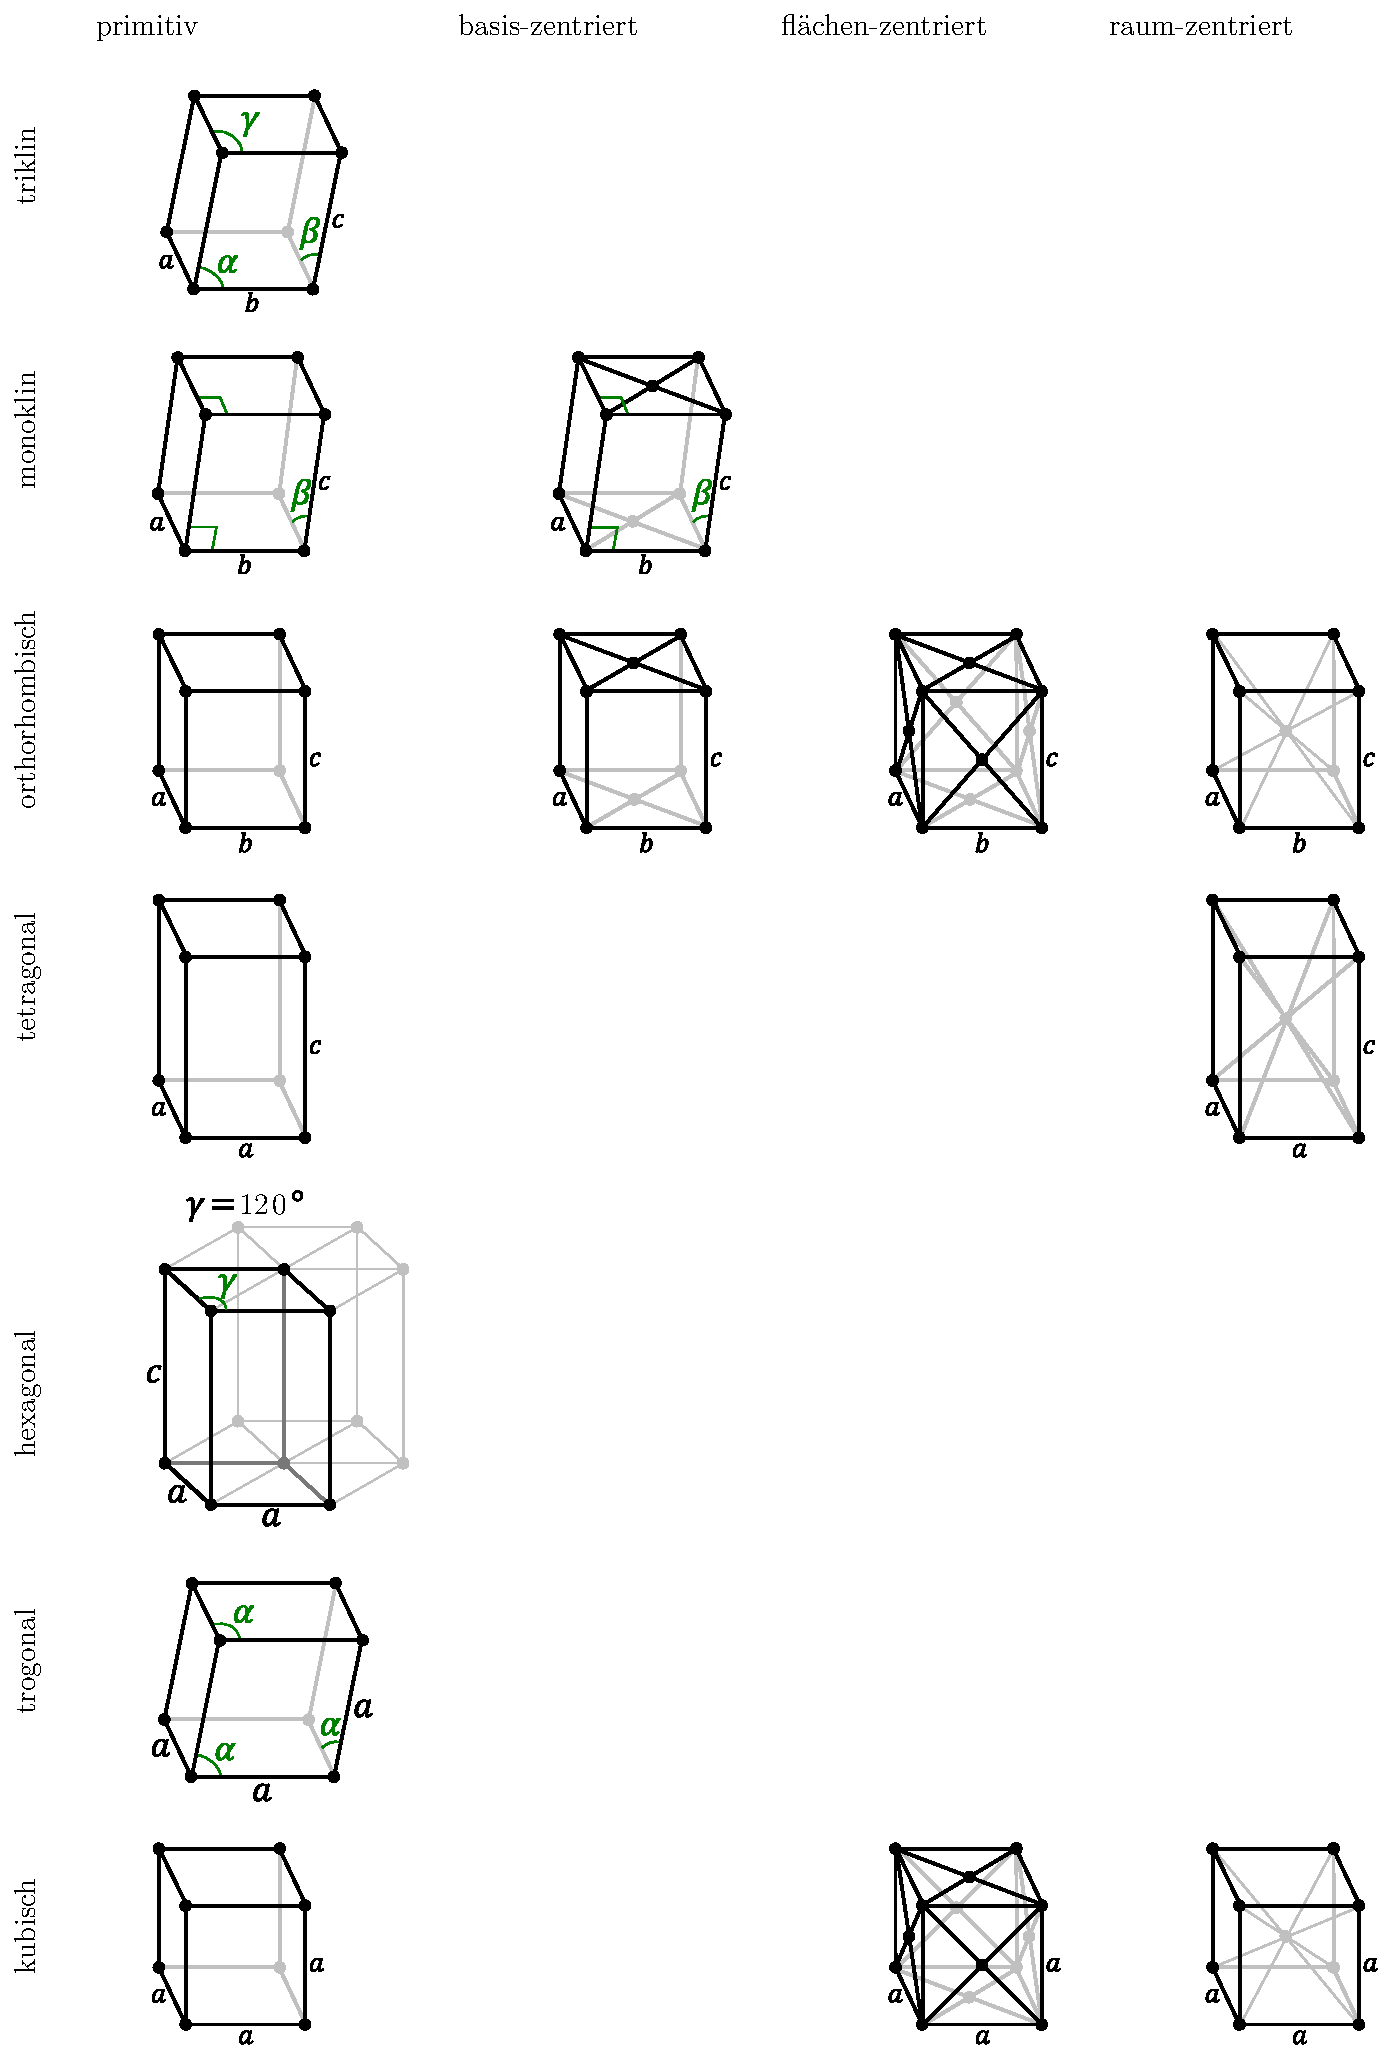
\includegraphics[height=\textheight]{\currfiledir kristall/bravais.pdf}
\inputtikz{\currfiledir bravais_ML}



\caption{Die 14 Bravais-Gitter \label{fig:gitter_bravais14}.  Gezeigt sind die konventionellen Einheitszellen, die die Symmetrie  des Gitters möglichst gut wiedergeben, aber im Falle der zentrierten Gitter nicht primitiv sind.
}
\end{figure}


\section{Die Basis}


Während das Gitter ein mathematisches Konstrukt ist, eine symmetrische Anordnung von mathematischen Punkten im dreidimensionalen Raum, kommt durch die \emph{Basis} die Natur ins Spiel. Die Basis beschreibt die Position der Atome relativ zum Gitterpunkt. Es kann dabei ein oder mehrere Atome in einer Basis sein. Die Position des Atoms $j$ relativ zum zugehörigen Gitterpunkt ist dann 
\begin{equation}
 \mathbf{r}_j = x_{1,j} \mathbf{a}_1 + x_{2,j} \mathbf{a}_2 + x_{3,j} \mathbf{3}_1  
\end{equation}
mit $0 \le x_{i,j} \le 1$. Die Lage der Atome in der Basis relativ zu 'ihrem' Gitterpunkt ist nicht eindeutig, da die Gitterpunkte ja mathematische Konstrukte und daher nicht messbar sind.


Die Symmetrie der Basis hat einen Einfluss auf die Symmetrie des Kristalls. Die sieben Kristallsysteme des mathematischen Gitters werden 32 kristallographische Punktgruppen, wenn also Translationssymmetrie unberücksichtigt bleibt. Diese unterscheiden sich dann in den anderen oben genannten Symmetrie-Operationen.
Wenn wieder die Translationssymmetrie mit berücksichtigen wird ergeben sich 230 kristallographische Raumgruppen.


\section{Beispiel: Honigwaben-Gitter}

Als Beispiel betrachten wir ein zweidimensionales Honigwaben-Gitter wie in nebenstehender Abbildung gezeigt. Dieses Gitter ist kein Bravais-Gitter, auch wenn es sehr symmetrisch aussieht. Zwei benachbarte Gitter-Punkte unterscheiden sich darin, wie das Gitter in ihrer Umgebung orientiert ist. Das  Honigwaben-Gitter ist ein dreizählig rotationssymmetrisch Gitter mit einer zwei-atomigen Basis. Mit dieser Wahl ist das Gitter translationsinvariant. Die Lage der Atome in der Basis relativ zu 'ihrem' Gitterpunkt ist nicht eindeutig. DIe Skizze zeigt verschiedene Möglichkeiten. XXX



\begin{marginfigure}
\inputtikz{\currfiledir honigwabe}

\caption{Honigwaben-Gitter}
\end{marginfigure}


\section{Die Wigner-Seitz-Zelle}

Die Wahl der primitiven Einheitszelle ist nicht eindeutig. Mit der Wigner-Seitz-Zelle gibt es eine Konstruktionsvorschrift, mit der man immer auf eine eindeutige primitive Einheitszelle kommt.

Man wähle einen Gitterpunkt und konstruiere Verbindungslinien zu allen benachbarten Punkten. Auf diese Linien errichte man Mittelsenkrechten (im zweidimensionalen) bzw. eine zur Linie senkrechte Ebene in der Mitte der Linie (im dreidimensionalen). Durch diese Mittelsenkrechten bzw. Mittelebenen wird eine Fläche bzw. ein Volumen eingeschlossen, das den Startpunkt beinhaltet. Dies ist die Wigner-Seitz-Zelle.

Diese Zelle ist primitiv, da sie nur einen Gitterpunkt beinhaltet. Sie hat außerdem die gleiche Symmetrie wie das Gitter selbst. Die Konstruktionsvorschrift ist unabhängig von der konkreten Wahl der Gittervektoren. Die Abbildung XXX zeigt als Beispiel die Konstruktion in einem schiefwinkligen zweidimensionalen Gitter sowie die Wigner-Seitz-Zelle des kubisch-raumzentrierten Gitters.

\begin{marginfigure}
\inputtikz{\currfiledir wsz-2d}

\caption{WSZ analog Hunklinger Fig. 3.30}
\end{marginfigure}




\section{Wichtige Kristallstrukturen}


\paragraph{\ch{NaCl}}
Kristallines \ch{NaCl} besteht aus einem flächen-zentrierten kubischen Gitter (engl: face-centered cubic, fcc). Schon weil es zwei verschiedene Atome sind muss es eine Basis mit mindestens zwei Atomen geben. Hier sind es genau zwei Atome,  beispielsweise mit \ch{Na+} im Ursprung und \ch{Cl-} im Zentrum der konventionellen Einheizstelle, also bei
\begin{equation}
 \mathbf{r}_{Cl} = \frac{1}{2} \left(\mathbf{a}_1 + \mathbf{a}_2 +  \mathbf{a}_3  \right)
\end{equation}
wenn die $\mathbf{a}_i$ so gewählt sind, dass sie die konventionelle Einheitszelle aufspannen, also kartesisch sind. Dies ist auch die Struktur von \ch{LiF}, \ch{MgO}, \ch{CaTe}.



\paragraph{\ch{CsCl}}
Dies ist ein primitives kubisches Gitter (engl. simple cubic, sc), ebenfalls mit einer zwei-atomigen Basis mit 
\begin{equation}
 \mathbf{r}_{Cl} = \frac{1}{2} \left(\mathbf{a}_1 + \mathbf{a}_2 +  \mathbf{a}_3  \right)
\end{equation}
Dies ist auch die Struktur von \ch{CsI}, \ch{TlBr}.

\paragraph{\ch{Fe}} Eisen bildet ein kubisch-raumzentriertes Gitter (engl. body-centered cubic, bcc) mit nur einem Atom in der Basis.

\paragraph{Diamant} Kohlenstoff-Atome in einem Diamant-Kristall bilden ein fcc-Gitter (face-centered cubic), aber ebenfalls mit einer zwei-atomigen Basis. Eine Basis kann also auch identische Atome beinhalten. Die Positionen sind der Ursprung sowie um ein Viertel der Raum-Diagonalen verschoben in der konventionellen Einheitszelle, als
\begin{align}
 \mathbf{r}_{C_1} = & 0 \\
 \mathbf{r}_{C_2} = & \frac{1}{4} \left(\mathbf{a}_1 + \mathbf{a}_2 +  \mathbf{a}_3  \right)
\end{align}
Die Atome sind untereinander in der tetraederförmigen Bindung der $sp^3$-Hybridisierung verbunden. Dies ist auch die Struktur von \ch{Si}, \ch{Ge}.

\paragraph{\ch{ZnS}} Zinkblende (\ch{ZnS}) hat die gleiche Struktur wie Diamant. Jede Atomsorte bildet für sich ein fcc-Gitter. Gegeneinander sind die Gitter um ein Viertel der Raum-Diagonalen verschoben. Dies ist auch die Struktur von \ch{CdTe}, \ch{GaAs}, \ch{InP}.


\section{Dichteste Kugelpackung}

Man kann die Atome in einem Kristallgitter durch harte Kugeln ersetzen und dabei den Kugeldurchmesser maximal wählen, also so, dass die Kugeln sich berühren. Welcher Volumenanteil des Kristalls wird nun durch Kugeln ausgefüllt? Die maximale Packungsdichte ist 
\begin{equation}
 \frac{\pi}{3 \sqrt{2}} \approx 74 \%
\end{equation}
Um diese Packungsdichte zu erreichen, liegen die Kugeln in der untersten Lage A in einem zweidimensionalen hexagonalen Gitter. Jede Kugel ist also von fünf Nachbarn umgeben. In der nächsten Lage B liegen die Kugeln in den Mulden, die sich zwischen den unteren Kugeln bilden.  Die Größe der Kugeln erzwingt, dass nur jeder zweite Mulde besetzt wird.
Dies ist wieder ein zweidimensionales hexagonales Gitter. Für die dritte Lage gibt es zwei Möglichkeiten: entweder man besetzt die Mulden, die den Positionen in Lage A entsprechen, oder man besetzt die Mulden, die weder von der Lage A noch von der Lage B eingenommen werden. Im ersten Fall spricht man von der ABAB-Stapelfolge, im zweiten von der ABCABC-Folge.

Welchen Bravais-Gittern entsprechen diese Folgen?  Die Folge ABCABC bildet ein flächen-zentriert kubisches Gitter (fcc).  Die Raumdiagonale der  Einheitszelle steht senkrecht auf den Ebenen A, B und C. Diese Packung wird daher auch 'cubic closed packing' (ccp) genannt. Die Folge ABAB nennt man  'hexagonal closed packing' (hcp), weil sie ein (dreidimensionales) hexagonales Bravais-Gitter mit einer zwei-atomigen Basis bildet (mit $c=a \sqrt{8/3}$, siehe Abb. XXX). Eine Kugel ist dabei am Ursprung der konventionellen Einheitszelle, die zweite bei 
\begin{equation}
 \mathbf{r}_{S_2} =  \frac{2}{3}  \mathbf{a}_1 + \frac{1}{3}  \mathbf{a}_2 + \frac{1}{2}  \mathbf{a}_3  
\end{equation}
 wobei die $\mathbf{a}_i$ die konventionelle Einheitszelle aufspannen.

Die kubische dichteste Kugelpackung wird beispielsweise von \ch{Au} und \ch{Ag} realisiert, die hexagonal dichteste Kugelpackung von \ch{Cd} oder \ch{Mg}. Es finden sich auch komplexere Abfolgen der Positionen A, B und C. Metalle aus der Gruppe der seltenen Erden bilden beispielsweise ABACABAC.


%-------------------




\printbibliography[segment=\therefsegment,heading=subbibliography]

%\renewcommand{\lastmod}{April 29, 2020}

\chapter{Das reziproke Gitter}





\section{Ziele}

\begin{itemize}
\item Sie dewe

\item S.

\end{itemize}


%\begin{figure}
%\inputtikz{\currfiledir fig_bodipy}
%  \caption{Absorptions- und Fluoreszenz-Spektrum des Farbstoffs BODIPY  (\href{https://www.thermofisher.com/de/de/home/life-science/cell-analysis/labeling-chemistry/fluorescence-spectraviewer.html?SID=srch-svtool&UID=10001moh}{thermofischer.com}).}
%\end{figure}



\section{Überblick}

Von den in Ka

%-------------------




\printbibliography[segment=\therefsegment,heading=subbibliography]

%%\renewcommand{\lastmod}{April 29, 2020}

\chapter{Phononen}





\section{Ziele}

\begin{itemize}
\item Sie können die  Dispersionsrelation $\omega = f(\mathbf{k})$ von Phononen (Abb. \ref{fig:phonon_intro}) benutzen, um die kollektive Bewegung der Atome zu beschreiben, und diese mit einfachen Modellen vergleichen.

\item Sie können die Teilchen-Eigenschaft von Phononen in Streuexperimenten erklären.

\end{itemize}




\begin{marginfigure}
\inputtikz{\currfiledir fig_gaas_intro}
\caption{Phononen-Dispersion in Gallium-Arsenid (\ch{GaAs}) (Daten aus \cite{Strauch_gaas}). \label{fig:phonon_intro}}

\end{marginfigure}


\section{Wie misst man das?}

Wir betrachten in diesem Kapitel eine kollektive Anregung aller Atome eines Kristalls in ihrer Schwingung um die Gleichgewichtsposition, die wir in den letzten beiden Kapitel betrachtet hatten. Dies entspricht den Normalmoden, die wir in der Molekülphysik bei der Schwingung der Moleküle betrachtet hatten. Nur versuchen wir hier nicht, eine Matrix zu diagonalisieren, sondern machen (raten) gleich einen passenden Ansatz. Wir werden sehen, dass die Anregung dieser Normalmoden nicht nur in ihrer Energie quantisiert ist ($E= (n + \frac{1}{2}) \hbar \omega$ überrascht wahrscheinlich nicht). Vielmehr benimmt diese Anregung der  Normalmoden sich wie ein punktförmiges Teilchen, das einen Impuls besitzt und mit dem man bei einem Stoß Energie und Impuls austauscht. Dieses Teilchen nennt man \emph{Phonon}.

Um Phononen zu vermessen, muss man also andere Teilchen an ihnen stoßen und Energie- und Impulsübertrag messen. Wegen des Welle-Teilchen-Dualismus kann man das auch als inelastische Streuung einer Welle am schwingenden Kristall beschreiben. Das ist die gleiche Streutheorie wie im letzten Kapitel, nur erlauben wir jetzt schwingende Atome und dadurch einen Energieübertrag.

\begin{marginfigure}
%\inputtikz{\currfiledir fig_gaas_intro}
\caption{3-Achs-Spektrometer}

\end{marginfigure}

Im Experiment macht man das beispielsweise durch inelastische Neutronenstreuung. Ein Neutronenstrahl wird in einem Kernreaktor oder in einer Spallationsquelle  hergestellt. Wichtig ist dabei, dass die Neutronen 'thermisch' sind, die kinetische Energie pro  Neutron also in etwa $k_B T$, also einige 10 meV beträgt. Diesen Neutronenstrahl leitet man in ein 3-Achs-Spektrometer. Dabei wird drei mal die Bragg-Beugung benutzt und jedes Mal der Winkel $\Theta$ des Strahls zu einem Kristall eingestellt. Die erste Bragg-Beugung wird benutzt, um eine Energie / Wellenlänge des Neutronenstrahls durch ihren Beugungswinkel zu selektieren. Am zweiten Kristall findet dann die inelastische Streuung statt. Hier werden die Phononen untersucht, und Ausbreitungsrichtung und Energie der Neutronen ändert sich. Die Richtung wird durch eine Reihe von Abschirmungen geometrisch festgelegt. Die Energieänderung wird gemessen, in dem an einem dritten Kristall wieder Bragg-Beugung zur Energiebestimmung benutzt wird. Schließlich muss man nur die die ankommenden Neutronen zählen. Man trägt das Ergebnis wie in Abb.~\ref{fig:phonon_intro} auf, als Energieänderung des Neutronen (=Frequenz der Phononen) über die Richtungsänderung der Neutronen (= Wellenvektor der Phononen).

\section{Einfaches Modell: lineare Kette}

Wir stellen die Schwingung der einzelnen Atome in einem Kristall als Superposition von ebenen Wellen dar. Die Atome bilden Ebenen, und alle Atome einer Ebene werden in gleichere Weise (Richtung und Amplitude) aus ihrer Ruhelage ausgelenkt. Die Schwingung findet also um eine Gleichgewichtsposition herum statt, die durch das in den letzten beiden Kapiteln beschriebene Gitter definiert ist. Wir nehmen ebenfalls an, dass die Schwingung harmonisch ist, was bei kleinen Auslenkungen sicherlich der Fall ist. Die Wahl der Kristall-Ebene bestimmt die Richtung des Wellenvektors $\mathbf{k}$ der ebenen Welle. Die Wellenlänge $\lambda$ den Betrag des Vektors $|\mathbf{k}| = 2 \pi / \lambda$. Weil alle Atome in der Ebene das gleiche tun, ist es möglich, allein eine lineare Kette von Atomen zu betrachten, zu der aus jeder Ebene nur jeweils ein Atom beiträgt.

Wir beschränken uns hier zunächst auf eine Auslenkung allein entlang der Richtung der Kette. Wir indizieren im Folgenden die Atome entlang der Kette mit den Indizes $s$ und $p$. Die Auslenkung eines Atoms an der Position $s$ aus der Gleichgewichtsposition sei $u_s$. 
Das zeitliche Mittel über $u_s(t)$ ist damit Null. Die Atome seien durch Federn verbunden. Die Kraft auf das Atoms $s$ ist dann
\begin{equation}
F_s = \sum_p \, c_p \left( u_{s+p} - u_s \right)
\end{equation}
mit der Federkonstante $c_p$, die beschreibt, die das betrachtete Atom mit dem $p$ Gitterpositionen weiter verknüpft ist. Es geht also nur die relative Auslenkung der Atome zueinander ein. Die Bewegungsgleichung wird damit
\begin{equation}
M \frac{d^2 \, u_s}{dt^2} = \sum_p \, c_p \left( u_{s+p} - u_s \right)
\end{equation}
wobei wir angenommen haben, dass alle Atome die gleiche Masse $M$ besitzen. Mit dem Ansatz einer ebenen Welle\sidenote{entsprechend den Nornmalmoden in der Molekülphysik} wird die Auslenkung des Atoms mit den Index $s+p$ zu
\begin{equation}
u_{s+p} = U_0 \, e^{-i ( \omega t - \mathbf{k} \cdot \mathbf{a} (s+p) )}
\end{equation}
mit dem Wellenvektor $\mathbf{k}$ im reziproken Raum und dem Gittervektor $\mathbf{a}$ im Realraum. Der Term $\mathbf{a} (s+p)$ beschreibt also die  Gleichgewichtsposition des betrachteten Atoms im Realraum, also das, was wir in den letzten beiden Kapiteln diskutiert hatten. Wenn wir diesen Ansatz in die Bewegungsgleichung einsetzen erhalten wir
\begin{equation}
- \omega^2 \, M = \sum_p \, c_p \left( e^{i \mathbf{k} \cdot \mathbf{a} p} - 1 \right)
\end{equation}
Da ja alle Atome identisch sind, gilt $c_p = c_{-p}$ und damit
\begin{equation}
 \omega^2 =  \frac{2}{M} \, \sum_{p=1}^\infty \, c_p \left( 1 - \cos ( \mathbf{k} \cdot \mathbf{a} p ) \right)
\end{equation}
Den hier gefundenen Zusammenhang zwischen Eigenfrequenz $\omega$ der Oszillation und Länge (und Richtung) des Wellenvektors $\mathbf{k}$ nennt man \emph{Dispersionsrelation}.





\section{Allein nächste Nachbarn wechselwirken}

Nun machen wir zusätzlich die Annahme, dass nur nächste Nachbarn miteinander wechselwirken, dass es also nur Federn zwischen direkt benachbarten Atomen gibt. Damit sind nur dir $c_{\pm 1}$ von Null verschieden und die Summe fällt weg. Wir ziehen jetzt auch die Wurzel und erhalten
\begin{equation}
\omega = \sqrt{\frac{4 \, c_1}{M}} \left| \sin (\frac{1}{2} \, \mathbf{k} \cdot \mathbf{a}  ) \right|
\end{equation}

\begin{marginfigure}

\inputtikz{\currfiledir kette_1atom}
\caption{Dispersionsrelation der einatomigen Kette}
\end{marginfigure}


\paragraph{Grenzfall langer Wellenlänge} Falls die Wellenlänge der ebenen Welle gegen unendlich geht, dann geht $k = 2 \pi \ \lambda$  gegen Null. Damit wird das Argument des Sinus sehr klein gegen Eins und wir können die Kleinwinkelnäherung anwenden:
\begin{equation}
\omega = \sqrt{\frac{4 \, c_1}{M}} \frac{1}{2}  |\mathbf{k}| | \mathbf{a}| \propto k
\end{equation}
Die Dispersionsrelation ist in der Nähe von $k = 0$ also linear in $k$. Die Schallgeschwindigkeit $v$ ist frequenzunabhängig
\begin{equation}
 v = \frac{\omega}{k} = a  \sqrt{\frac{ c_1}{M}}  = \text{const.}
\end{equation}



\paragraph{Physikalisch bedeutsamer Bereich von $\mathbf{k}$} 

\begin{marginfigure}
\inputtikz{\currfiledir outside_BZ}

\caption{Eine Welle mit dem Wellenvektor $k + G = k + 2\pi /a$ beschreibt die gleiche Auslenkung der Atome wie die mit dem Wellenvektor $k$.  Vektoren innerhalb der ersten Brillouinzone sind ausreichend, um alle möglichen Bewegungsmuster zu beschreiben. \label{fig:phonon_k_plus_g} }
\end{marginfigure}


Wir betrachten das Verhältnis der Auslenkung benachbarter Atome, also
\begin{equation}
 \frac{u_{s+1}}{u_s}  = 
 \frac{U_0 e^{i \mathbf{k} \cdot \mathbf{a} (s+1) } } 
        {U_0 e^{i \mathbf{k} \cdot \mathbf{a} s}} 
         = e^{i \mathbf{k} \cdot \mathbf{a}}
\end{equation}
Dieser Ausdruck ist periodisch in $\mathbf{k}$. Alle möglichen Werte werden bereits abgedeckt im Intervall $- \pi < \mathbf{k} \cdot \mathbf{a}  < \pi$, bzw. in einer Dimension 
 \begin{equation}
 - \frac{\pi}{a} < k <  \frac{\pi}{a}
 \end{equation} 
Dies ist gerade die erste Brillouin-Zone. Werte von $k$ außerhalb dieser Zone beinhalten keine weitere Information. Sie beschreiben die gleiche Auslenkung der Atome. Die Funktion  $e^{i \mathbf{k} \cdot \mathbf{a}}$ wird nur an den Gitterpositionen ausgewertet. Welchen Wert sie an anderer Stelle annimmt spielt keine Rolle. Für $k$ außerhalb der ersten Brillouin-Zone oszilliert die Funktion zwischen den Gitterpositionen schneller, was aber keine physikalische Konsequenz hat.



\paragraph{Gruppengeschwindigkeit}
Die Gruppengeschwindigkeit beschreibt die Geschwindigkeit eines Wellenpakets und damit die Ausbreitung von Information
\begin{equation}
v_g = \frac{d \omega}{d k} =
 \sqrt{\frac{c_1 \, a^2}{M} } \, \cos 
 \left( \frac{1}{2} \mathbf{k} \cdot \mathbf{a} \right)
\end{equation}
An den Grenzen der Brillouin-Zone, bei $k = \pm \pi / a$ wird damit die Gruppengeschwindigkeit Null. Dies entspricht einer stehenden Welle.






\section{Lineare zweiatomige Kette}

Nun heben wir die Annahme auf, dass alle Atome identisch sind. Wir betrachten eine Kette, die abwechselnd aus zwei Atomsorten besteht. In der Sprache eines Gitters ist hat diese also eine zweiatomige Basis. Die Gitterkonstante $a$ ist der (kürzest) Abstand zwischen \emph{identischen} Atomen. Hier nehmen wir an, dass sich die Atome in ihrer Masse unterscheiden. Die Federn seien aber wieder nur zwischen nächsten Nachbarn (also verschiedenen Atomsorten) und sie seine alle identisch\sidenote{Man könnte auch identische Massen und alternierende Federn annehmen.} Der Index $s$ bezeichnet nun die Einheitszelle (nicht das Atom). Wir unterscheiden zwischen den Atomen, in dem die eine Sorte um $u_s$, die andere um $v_s$ ausgelenkt sein soll.  Die Reihenfolge entlang der Kette ist also $u_{s-1}$ ---  $v_{s-1}$ --- $u_{s}$ ---  $v_{s}$ --- $u_{s+1}$ ---  $v_{s+1}$. Damit werden die Bewegungsgleichungen
\begin{align}
 M_1 \frac{d^2 u_s}{dt^2} = & c \, \left( v_s + v_{s-1} - 2 u_s \right) \\
 M_2 \frac{d^2 v_s}{dt^2} = & c \, \left( u_s + u_{s-1} - 2 v_s \right) 
\end{align}
wobei $c$ hier die einzige Federkonstante bezeichnet ($c_1$ von oben) und die $M_{1,2}$ die Masse der beiden Atomsorten ist.
Wir machen den Ansatz
\begin{align}
  u_s   = & u \,   e^{i \mathbf{k} \cdot \mathbf{a}  s} \, e^{-i \omega t} \\
  v_s  = & v  \, e^{i \mathbf{k} \cdot \mathbf{a}  s} \, e^{-i \omega t}
\end{align}
und erhalten zwei Lösungen für die Eigenfrequenz $\omega$ und damit die Dispersionsrelation
%\begin{equation}
%\omega^2 = c \, \frac{M_1 + M_2}{M_1 M_2}
%\pm \frac{c}{M_1 M_2} \sqrt{ (M_1 + M_2)^2 - 4 M_1 M_2 \sin^2 \left( \frac{1}{2}  \mathbf{k} \cdot \mathbf{a} \right) } 
%\end{equation}
%oder
\begin{equation}
\omega^2 =  \frac{c}{\mu}
\pm c \sqrt{ \frac{1}{\mu^2} - \frac{4}{M_1 M_2}  \sin^2 \left( \frac{1}{2}  \mathbf{k} \cdot \mathbf{a} \right) } 
\end{equation}
mit der reduzierten Masse $\mu = (M_1  M_2)/(M_1 + M_2)$. Die Dispersionsrelation besteht also aus zwei Zweigen, je nach Vorzeichen des $\pm$: Das negative Vorzeichen beschreibt den \emph{akustischen Zweig}. Er geht exakt in die einatomige Kette über, wenn man $M_1 = M_2$ setzt und $a$ entsprechend anpasst. Auch für $M_1 \neq M_2$ ist der akustische Zweig sehr ähnlich der einatomigen Kette, insbesondere linear zu $k$ in der Nähe von $k=0$. Das positive Vorzeichen beschreibt den \emph{optischen Zweig}. Für $k \rightarrow 0$ geht hier die Frequenz $\omega$ nicht gegen Null sondern gegen $\sqrt{2 c / \mu}$. Am Rand der Brillouin-Zone, also bei $k = \pi /a $ wird der Sinus Eins und damit\sidenote{Man zieht den Term $M_1 - M_2$ aus der Wurzel und macht dabei die Annahme $M_1 > M_2$.}
\begin{align}
\omega_+ = & \frac{2 c}{M_2} \\
\omega_- = & \frac{2 c}{M_1} 
\end{align}
Die Aufspaltung der Äste am Rand der Brillouin-Zone geht also mit dem Verhältnis der Massen $M_1 / M_2$. Diese Aufspaltung führt zu einer \emph{Bandlücke}: Im Frequenzbereich zwischen $\omega_- $ und $\omega_+$ gibt es keine Lösung der Bewegungsgleichung, unabhängig vom Wellenvektor $\mathbf{k}$. In einer solchen Kette von mit Federn verbundenen Massen können sich keine Wellen ausbreiten, deren Frequenz wischen $\omega_- $ und $\omega_+$ liegt. Wenn eine Masse von außen mit einer solchen Frequenz getrieben würde, dann bliebe diese Bewegung auf die nähere Umgebung beschränkt und weit entfernte Massen würden in Ruhe bleiben.




\begin{marginfigure}

\inputtikz{\currfiledir kette_2atom}
\caption{Dispersionsrelation der zweiatomigen Kette}
\end{marginfigure}

Die Bezeichnung der beide Äste als akustisch und optisch ergibt sich aus dem Schwingungsmuster bei kleinem $k$. Man findet
\begin{align}
 u = &v &&  \text{akustischer Zweig} \\
  \frac{u}{v} = &- \frac{M_2}{M_1} &&  \text{optischer Zweig} 
\end{align}
Im akustischen Zweig folgen also beide Atomsorten einer gemeinsamen Schwingungsmuster, wie man es für eine Schallwelle erwartet. Im optischen Zweig bleibt der Schwerpunkt ruhen ($u M_1 = - v M_2$). Wenn die beiden Atomsorten allerdings unterschiedliche (Teil-)Ladungen besitzen, dann führt diese Schwingung zu einem oszillierenden Dipolmoment und ist somit optisch anregbar, also Infrarot-aktiv.


\begin{marginfigure}
\inputtikz{\currfiledir muster}
\caption{Schwingungsmuster bei langen Wellenlängen: \textit{oben}: akustische Mode, \textit{unten}: optische Mode. Dargestellt ist jeweils die Auslenkung als Funktion des Ortes.}
\end{marginfigure}





\section{Moden im Dreidimensionalen}

Im allgemeinen Fall sind im dreidimensionalen diverse Schwingungsmoden vorhanden. Man kann diese wie folgt klassifizieren.

\paragraph{Transversal oder longitudinal} Die Auslenkung der Atome aus der Gleichgewichtsposition kann in Richtung des Wellenvektors $\mathbf{k}$ erfolgen (longitudinale Schwingung), oder senkrecht dazu (transversale Schwingung). Dabei ist die transversale Schwingung zweifach entartet, weil es zwei Richtungen gibt, die senkrecht auf $\mathbf{k}$ stehen.


\paragraph{Akustisch  oder optisch} Auch bei $p > 2$  Atomen in der Basis kann man wie im letzten Abschnitt verfahren. Man findet eine akustisch Mode, in der $u = v = w = \dots$, und $p -1$ optische Moden, in denen manche Atome außer Phase schwingen.

Zusammen ergeben sich damit folgende Moden \\
\begin{tabular}{rl}
$1$ & longitudinal akustisch (LA)\\
$2$ & transversal akustisch (TA) \\
$p-1$ & longitudinal optisch (LO) \\
$2(p-1)$ & transversal optisch (TO) \\
\end{tabular} \\
also insgesamt $3p$ Mode, wie man bei $p$ Atomen pro Basis und 3 Dimensionen erwarten würde.






\section{Streuung am schwingenden Gitter}

Wir betrachten noch einmal die Streuung einer Welle an einer Anordnung von Streuzentren, wie im letzten Kapitel, nur erlauben wir jetzt, dass die Streuzentren sich leicht um ihre Ruheposition bewegen
\begin{equation}
\mathbf{r}_m(t) = \mathbf{R}_m + \mathbf{u}_m(t) \quad \text{mit} \quad \left<\mathbf{u}_m(t)\right> = 0
\end{equation}
Die Amplitude der auslaufenden ebenen Welle mit der Richtungsänderung $\mathbf{K} = \mathbf{k}_\text{out} - \mathbf{k}_\text{in}$ ist
\begin{equation}
A_S(t) \propto e^{-i \omega_0 t} \, \sum_m e^{-i \mathbf{K} \cdot \mathbf{r}_m(t)} =
e^{-i \omega_0 t} \, \sum_m e^{-i \mathbf{K} \cdot \mathbf{R}_m}  e^{-i \mathbf{K} \cdot \mathbf{u}_m(t)}
\end{equation}
Da die Amplitude der Schwingung $\mathbf{u}_m(t)$ klein ist gegenüber der Gitterkonstanten und gilt für den interessanten Bereich von $\mathbf{K}$ dass  $\mathbf{K} \cdot\mathbf{u}_m(t) \ll 1 $. Daher können wir die zweite Exponentialfunktion in einer Reihe entwickeln und nach dem ersten Glied abbrechen.\sidenote{Das zweite Glied braucht man unten für den Debye-Waller-Faktor.}
\begin{equation}
 e^{-i \mathbf{K} \cdot \mathbf{u}_m(t)} \approx 1 - i \mathbf{K} \cdot \mathbf{u}_m(t)
\end{equation}
Die Auslenkungen $\mathbf{u}_m(t)$ beschrieben wir wieder wie oben als ebene Wellen, wobei wir hier den Wellenvektor $\mathbf{q}$ nennen statt $\mathbf{k}$, um ihn vom Vektor der gestreuten Welle zu unterscheiden. Der Einfachheit halber betrachten wir auch nur akustische Moden. Damit wird
\begin{equation}
\mathbf{u}_m(t) = \sum_\mathbf{q} \mathbf{U}_\mathbf{q} \, 
e^{ \pm i ( \mathbf{q} \cdot \mathbf{R}_m - \omega_\mathbf{q} t ) }
\end{equation}
Alles zusammen erhalten wir damit
\begin{equation}
A_S(t) \propto 
\sum_m e^{-i \mathbf{K} \cdot \mathbf{R}_m}  
e^{-i \omega_0 t} 
-
\sum_m \sum_\mathbf{q}  i \mathbf{K} \cdot \mathbf{U}_\mathbf{q} \,
 e^{-i (\mathbf{K} \pm \mathbf{q} ) \cdot \mathbf{R}_m}  
e^{-i (\omega_0 \pm \omega_\mathbf{q})  t} 
\end{equation}
Der erste Term ist die schon aus dem letzten Kapitel bekannte elastische Streuung. Hier geht die Bewegung der Streuzentren nicht ein. der zweite Term ist die inelastische Streuung, die proportional zur Amplitude $\mathbf{U}_\mathbf{q}$ der Schwingung der Streuzentren ist. Für die elastische Streuung hatten wir im letzten Kapitel gesehen, dass die Summe über alle Atompositionen nur dann einen Beitrag liefert, wenn die Bedingung $\mathbf{K} = \mathbf{G}$ erfüllt ist. Für die inelastische Streuung liefert die gleiche Argumentation die Bedingung
\begin{equation}
 \mathbf{K} \pm \mathbf{q} = \mathbf{G} \quad \text{und} \quad \omega_\text{out} = \omega_0 \pm \omega_\mathbf{q}
\end{equation}
Die Energie / Frequenz der gestreuten Welle ändert sich also bei inelastischer Streuung, wie beim Raman-Effekt in der Molekülphysik.



%\section{Inelastische Streuung}
%
%Im letzten Kapitel zur Strukturbestimmung hatten wir die Streuung von Röntgen-Strahlen oder andere (Materie-)Wellen benutzt. Dies war \emph{elastische} Streuung. Die Wellenlänge bzw. der Betrag des Wellenvektors $\mathbf{k}$ hat sich dabei nicht verändert, nur seine Richtung. Um die Phononen-Dispersion zu messen benötigen wir \emph{inelastische} Streuung. Gleichzeitig mit der Änderung der Richtung des Wellenvektors soll sich auch sein Betrag ändern. Dabei wird Energie von der Welle an die Gitterschwingung abgegeben oder davon aufgenommen. 

Die Bedingung lässt sich durch Multiplikation mit $\hbar$ als 
 Energie- und Impulserhalten schreibt 
\begin{align}
\hbar \omega_{out} = & \hbar \omega_{0}  \pm \hbar
 \omega_\mathbf{q} \\
\hbar \mathbf{k}_{out} =  &\hbar \mathbf{k}_{0} \pm \hbar 
\mathbf{q}  + \hbar \mathbf{G}
\end{align}
Dies ist ein wichtiger Schritt! Bei der Streuung (und anderen Effekten) verhalten sich Gitterschwingungen so als wären sie ein Teilchen. Dieses Teilchen nennt man \emph{Phonon}. Es hat die Energie $\hbar \omega_\mathbf{q}$ und den Impuls $\hbar \mathbf{q}$. Das positive Vorzeichnen beschreibt die Absorption (Vernichtung) eines Phonons, das negative die Emission (Erzeugung). Der Impuls $\hbar \mathbf{G}$ wird auf den gesamten Kristall übertragen, ohne dabei Energie zu übertragen.\sidenote{Wie beim Abprallen eines Balles von einer Wand.} Der Impuls des Phonons ist allerdings kein 'echter' Impuls, sondern nur ein Quasiimpuls oder Kristallimpuls, da ihm der Massetransport im Sinne von $p = m v$ fehlt. Manchmal nennt man das Phonon ein 'Quasiteilchen', manchmal ist dieser Term aber auch für modifizierte ('dressed') elementare Teilchen reserviert.\sidenote{Siehe 'quasiparticle' in engl. wikipedia.} Zumindest beschreibt es eine kollektive Anregung und ist damit ein Boson, weil natürlich eine Gitterschwingung mehr oder weniger stark angeregt sein kann und somit viele identische Phononen existieren können.






\section{Experimente}

Man kann inelastische Streuung genauso wie elastische Streuung mit diversen Arten von (Materie-)Wellen betreiben. Diese unterscheiden sich aber in ihre Energie bei gegebener Wellenlänge. Da bei inelastische Streuung am Ende ein Energieunterschied von $\hbar
 \omega_\text{phonon} $ gemessen werden soll, fällt dies je nach Art der Welle mehr oder weniger schwierig aus.
 
 \begin{table}
 \begin{tabular}{lll}
          & Wellenlänge & Energie \\
   Laser & 5320 \AA & 2.3 eV \\
   Röntgen & 0.1 \AA & 100 keV \\
   Neutronen & 1 \AA & 100 meV \\
 \end{tabular}
 \caption{Typische Energien und Wellenlängen}
 \end{table}

Bei der Dispersionsrelation der Phononen ist der relevante Bereich des Wellenvektors $q$ durch die erste Brillouin-Zone, also $| q | \le \pi / a$ gegeben.  Die Änderung des Wellenvektors der (Materie-)Welle $\mathbf{K}$ ist vom Betrag her maximal $4 \pi / \lambda$ (von $+\mathbf{k}_0$ zu $-\mathbf{k}_0$). Daher muss die Wellenlänge $\lambda$ sinnvollerweise kleiner als $2a$ sein, also im Bereich von wenigen Angstrom liegen.
 Die Wellenlänge von sichtbarem Licht ist also viel zu lang, um die gesamte Brillouin-Zone abzudecken. Energieänderungen  von einigen meV sind im Sichtbaren aber noch gut zu messen. Bei Röntgenstrahlen wird dies sehr schwierig, so dass Neutronenstreuung die Methode der Wahl ist, da hier die Energie der Phononen eine deutliche Änderung der Energie der Neutronen bewirkt.




\section{Inelastische Neutronenstreuung}


Die Streubedingung konstruiert man auch im inelastischen Fall mit der Ewald-Kugel, wie im letzten Kapitel. Nur kommt hier nun zusätzlich der Vektor $\mathbf{q}$ des Phonons hinzu, der entweder zu $\mathbf{k}_0$ addiert oder subtrahiert wird. Je nach dem liegt $\mathbf{k}$ dann entweder innerhalb\sidenote{$|k|$ kleiner, $\lambda$ größer, $\omega$ kleiner als im einfallenden Strahl, also Emission eines Phonons} oder außerhalb der Kugel, aber nicht mehr auf der Ewald-Kugel wie im elastischen Fall.

Man misst also für jede Richtungsänderung $\mathbf{K}$ die Änderung der Energie / Frequenz des Neutronenstrahls. Zusammen mit der bekannten Struktur und Orientierung des Kristallgitters und damit der Gittervektoren $\mathbf{G}$ kann man so die vollständige Dispersionrelation der Phononen bestimmen.

\begin{marginfigure}
\inputtikz{\currfiledir ewald_inelastisch}
\caption{Ewald Kugel inelastisch}
\end{marginfigure}




\newpage

\section{Beispiel: Kupfer}




\begin{marginfigure}
\inputtikz{\currfiledir fcc-3d_2x}
\caption{Punkte hoher Symmetrie in der Brillouin-Zone werden durch große Buchstaben gekennzeichnet. der $\Gamma$-Punkt ist die Mitte der BZ, also $k=0$. Der Pfad $\Gamma$--X--K--$\Gamma$--L nutzt aus, das Punkte mehrfach  vorkommen. \label{fig:phonon_pfad} }
\end{marginfigure}


Kupfer bildet einen kubisch-flächenzentrierten Kristall mit einatomiger Basis. Der reziproke Raum ist also kubisch-raumzentriert. Die Gitterkonstante beträgt 3.6~\AA. Abb. \ref{fig:phonon_kupfer} zeigt die Dispersionsrelation der Phononen, die durch inelastische Neutronenstreuung gemessen wurde. Aufgetragen ist die Frequenz $\nu$ des Phonons (aus der Änderung der Energie der Neutronen) über dem Wellenvektor $\mathbf{q}$, der sich aus der Änderung des Wellenvektors des Neutronenstrahls ergibt. Der Wellenvektor $\mathbf{q}$ ist in Form seines Miller-Indexes angegeben, der ja gerade den Vorfaktoren vor den primitiven reziproken Gittervektoren $\mathbf{b}_i$ entspricht. Die horizontale Achse ist mit dem Wert $\zeta$ beschriftet, der ein- oder mehrmals im Miller-Index vorkommt. Alle
 dargestellten Wellenvektoren sind damit entweder parallel zu einem reziproken Gittervektor (erstes Intervall), parallel zur Flächendiagonalen (zweites Intervall) oder parallel zur Raumdiagonalen (drittes Intervall). Die horizontale Achse ist entsprechend dem Betrag des Wellenvektors 
 $|\mathbf{q}|$ skaliert, d.h. der Abstand $\zeta = 0 \dots 0.5$ verhält sich wie $1$ zu $\sqrt{2}$ zu $\sqrt{3}$. Die gesamte Abbildung stellt die Frequenz der Phononen entlang einem Pfad im reziproken Raum dar, der in Abbildung \ref{fig:phonon_pfad}  dargestellt ist. Dabei kann man ausnutzen, dass reziproke Gittervektoren $\mathbf{G}$ addiert werden können ohne etwas  zu verändern (siehe Abb. \ref{fig:phonon_k_plus_g})
 
	\begin{figure}
\inputtikz{\currfiledir fig_copper_all}
\caption{Phononen-Dispersion in Kupfer (Daten aus \cite{Svensson_cu}). \label{fig:phonon_kupfer}}
\end{figure}

Die Dispersionsrelation ähnelt zumindest in Richtungen hoher Symmetrie, also [001] und [111]	dem einfachen Modell der linearen einatomigen Kette. Es gibt nur akustische Zweige, weil nur ein Atom in der Basis vorhanden ist. Die transversalen Moden sind entlang der hoch-symmetrischen Richtungen zweifach entartet. In die Richtung [110] wird die Entartung aufgehoben.


\section{Beispiel: Galliumarsenid (\ch{GaAs})}


Galliumarsenid (\ch{GaAs}) besitzt ebenfalls eine kubisch-flächenzentrierte Kristallstruktur, aber mit einer zweiatomigen Basis, eben eine Zinkblende-Struktur. Die Gitterkonstante der konventionellen Einheitszelle beträgt 5.7~\AA. Die Abbildung zeigt analog zu oben die Dispersionrelation. Wir finden nun auch einen optischen Zweig, da zwei Atome in der Basis sind. Die transversalen Zweige sind wieder in die hoch-symmetrische [001] und [111] Richtung entartet. In die [110] Richtung ist diese Entartung aufgehoben und wir finden 6 Zweige (2 Atome mal 3 Raumrichtungen).


\begin{figure}
\inputtikz{\currfiledir fig_gaas_all}
\caption{Phononen-Dispersion in \ch{GaAs} (Daten aus \cite{Strauch_gaas} ).}
\end{figure}



\section{Inelastische Streuung von Licht: Raman und Brillouin}

Der Wellenvektor eines sichtbaren Photons ist viel kürzer als der Rand der Brillouin-Zone also
\begin{equation}
 k_\text{Licht} = \frac{2 \pi}{\lambda} \ll k_\text{phonon} \approx \frac{\pi}{a}
\end{equation}
Das Verhältnis ist etwa 1:1000. Wenn man die Dispersionsrelation von Phononen und Photonen ins gleiche Diagramm zeichnet, dann sind die Photonen ein quasi senkrechter Strich. Mit sichtbarem Licht kann man daher die Dispersionsrelation der Phononen nur in der Nähe von $k \approx 0$ messen. Wenn dabei optische Phononen erzeugt oder vernichtet wird, dann entspricht dies der Raman-Streuung aus der Molekülphysik und Energieunterscheiden von Stokes- und Anti-Stokes-Linie von einigen 10 meV. Wenn akustische Phononen involviert sind, dann bezeichnet man dies als Brillouin-Streuung mit Energieunterscheiden von etwa 0.1 meV, die nur sehr aufwändig messbar sind.


\section{Anwendung: Akusto-optischer Modulator}

Akustische Phononen finden in Form des  akusto-optischen Modulators eine wichtige Anwendung in der Optik: eine laufende longitudinale Ultraschallwelle, also akustische Phononen, entspricht einer periodische Modulation des Brechungsindex des Materials. Dies ist damit ein Phasengitter für einen Lichtstahl, der senkrecht zur Ultraschallwelle durch das Material läuft. Der Lichtstahl wird damit an dem Gitter gebeugt und in verschiedene Ordnungen aufgespalten.

Dies kann auf verschiedene Weisen genutzt werden. In einfachsten Fall als Schalter: nur wenn die Ultraschallwelle anliegt existiert eine erste Beugungsordnung. Damit kann ein Strahl schnell (ns) an- und aus-geschaltet werden, wenn man den Ultraschall-Generator schaltet. Durch Variation der Amplitude der Ultraschallwelle kann eine beliebige Amplituden-Modulation des Lichtstahls erreicht werden.

Die Beugung in die erste Ordnung entspricht der Absorption eines Ultraschall-Phonons, die in die minus erste Ordnung der Emission. Damit ist klar, dass die Beugung auch mit einer Frequenzverschiebung einher geht. Es muss schließlich Energie- und Impuls-Erhaltung gelten. Auf diese Weise ist es möglich, sehr schmalbandige und frequenzstabile Laser im sichtbaren Spektralbereich (Frequenz ca. 300 THz) um die Frequenz des Phonons (ca. 10--100 MHz) zu verstimmen. Wenn man die Frequenz des  Ultraschall-Generators kontinuierlich ändert, dann kann man so einen kleinen Frequenzbereich kontrolliert abfahren.

Gleichzeitig ändert sich damit auch der Beugungswinkel. So kann ein Lichtstrahl sehr schnell in verschiedene, kontinuierlich änderbare Richtungen abgelenkt werden, was in manchen optischen Mikroskopen Verwendung findet.




%-------------------




\printbibliography[segment=\therefsegment,heading=subbibliography]

%%\renewcommand{\lastmod}{April 29, 2020}

\chapter{Wärmekapazität der Phononen}





\section{Ziele}

\begin{itemize}
\item Sie können das Konzept der Zustandsdichte benutzen, um damit die Wärmekapazität fester Stoffe zu erklären, wie unten für Kupfer gezeigt.

\item Sie können die Modelle von Einstein und Debye erklären und vergleichen, beispielsweise unter welchen Umständen welches bessere Ergebnisse liefert.

\end{itemize}


\begin{figure}
\inputtikz{\currfiledir dos_cv_Cu}
  \caption{ \textit{links:} Zustandsdichte von Phononen in Kupfer (dick) verglichen mit dem Debye-Modell (dünn). Daten digitalisiert aus \cite{Svensson_cu}. \textit{rechts:} Wärmekapazität von Kupfer verglichen mit der $T^3$-Abhängigkeit des Debye-Modells. Daten aus \cite{Data_notebook}. \label{fig:wk_kupfer}}
\end{figure}



\section{Wärmekapazität}


Die Wärmekapazität eines Stoffes beschreibt den Zusammenhang zwischen der Änderung der Temperatur $T$ durch die Änderung der inneren Energie $U$ beispielsweise durch Wärmezufuhr, also
\begin{equation}
 C_V = \left( \frac{\partial U}{\partial T} \right)_{V = \text{const.}}
\end{equation}
bei konstantem Volumen $V$ des Stoffes. Messtechnisch ist $C_P$, also die Wärmekapazität bei konstantem Druck $P$ einfacher, jedoch ist die theoretische Beschreibung von $ C_V $ einfacher. Bei Festkörpern ist der Unterschied gering, da diese sich (zumindest im Vergleich zu Gasen) wenig mit steigender Temperatur ausdehnen.

Im Experiment findet man, dass die Wärmekapazität fester Stoffe mit der Temperatur steigt und sich dem Wert des Gesetzes von Dulong-Petit annähert
\begin{equation}
 C_V = 3 \, N_A \, k_B \approx 25 \text{~J} \text{~mol}^{-1} \text{~K}^{-1} \quad .
\end{equation}
Der Verlauf von $ C_V$ bei niedrigeren Temperaturen ist eine einfach zu bestimmende makroskopische Größe, die viel über den mikroskopischen Aufbau des Festkörpers aussagt. Wir werden sehen, dass sie zumindest bei Nichtleitern vollständig durch die quantisierte  Gitterschwingungen und so die Teilcheneigenschaft der Phononen bestimmt ist. Das Modell dazu geht auf A.~Einstein zurück, auch wenn er bei der Zustandsdichte $D(\omega)$ vereinfachende Annahmen getroffen hat. Die Innere Energie $U(T)$ \textbf{pro Mode} ist
\begin{equation}
U(T) = \int_{\omega=0}^{\infty} \, \hbar \omega \, \braket{ n (\omega, T) } \, D(\omega) \, d\omega \label{eq:wk_u_allg} \quad .
\end{equation}
Bei jeder Frequenz $\omega$ existieren Phononen in der Dichte $D(\omega)$ der möglichen Zustände pro Frequenzintervall, der Energie pro Phonon $\hbar \omega$ und der Besetzung $\braket{ n (\omega, T) } $. Die Innere Energie ist dann das Integral über alle Frequenzen, und die Wärmekapazität die Ableitung davon nach der Temperatur $T$.


\section{Zustandsdichte im reziproken Raum $D(k) \, dk$ }

Zunächst betrachten wir nicht die eigentlich benötigte Zustandsdichte im Frequenzraum $D(\omega) d\omega$ sondern die im reziproken Raum $D(k) dk$. Die Argumentation und die Rechenschritte sind dabei dieselben, die auch bei der Herleitung der optischen Modendichte bei der Schwarzkörperstrahlung verwendet wurde\sidenote{z.B. Vorlesung EPB2 Atome, Kerne, Teilchen}, auf die wir weiter unten eingehen werden.

Bisher hatten wir uns über die Länge unsere ein- oder mehratomigen Kette keine Gedanken gemacht. Wenn sie endlich lang sein soll, was ja notgedrungen der Fall ist, dann können die Enden entweder frei sein, also keine Kraft auf sie wirken, also $\ddot{u} = 0$ sein. Oder sie können fest sein, also ohne Bewegung, also $u=0$. Eine dritte Möglichkeit sind periodische Randbedingungen, also eine ringförmige Kette mit $u_0 = u_N$ bei $N$ Atomen in der Kette. Wir benutzen hier diese Randbedingung, die anderen geben das gleiche Ergebnis. Die Auslenkung der Masse am Index $s$ ist mit dem Ansatz der ebenen Welle
\begin{equation}
 u_s = u \, e^{- i \omega \, t} \, e^{i s \mathbf{k} \cdot \mathbf{a}}
\end{equation}
mit dem Wellenvektor $\mathbf{k} $ im reziproken Raum und dem Gittervektor $\mathbf{a}$ im  Realraum. Die Randbedingung $u_0 = u_N$ erfordert dann
\begin{equation}
 N \, k \, a = 2 \pi \, n \quad ,
\end{equation}
wobei $n$ eine beliebige ganze Zahl ist und wir die Beträge der Vektoren eingesetzt haben.
Die Gesamtlänge der Kette ist $L = N a$. Damit kann $k$ nur diskrete Werte annehmen, die den Abstand $\Delta k$ haben
\begin{equation}
\Delta  k = \frac{2 \pi }{L}  \quad .
\end{equation}
Die Dichte $ D(k) \, dk$ der möglichen Werte von $k$ auf der $k$-Achse ein Wert pro $\Delta k$, also
\begin{equation}
 D(k) \, dk = \frac{L}{2 \pi} \, dk  \quad .
\end{equation}
Die Zustandsdichte ist im $k$-Raum also konstant.
Analog kann man im Zwei- oder Dreidimensionalen verfahren, also bei Quadraten oder Kuben der Kantenlänge $L$. Die Zustandsdichte ist
\begin{equation}
D(k) = \frac{N_\text{PEZ}}{V_{BZ}}  = 
\frac{V_\text{Kristall}} {(2 \pi)^d} =
 \left(\frac{L}{2 \pi} \right)^d 
\end{equation}
mit der Dimensionalität $d$ und der Anzahl der \textbf{primitiven} Einheitszellen $N_\text{PEZ}$. Das ist wie oben die Zustandsdichte für eine Art der Bewegung. Bei $p$ Atomen je Einheitszelle gibt es $3p$ Äste in der Dispersionsrelation und die Gesamt-Zustandsdichte ist entsprechend größer.

Was ist hier passiert? Die physikalisch sinnvollen Werte von $k$ waren schon im letzten Kapitel nach oben beschränkt, weil es nicht hilft, wenn die Welle schneller oszilliert als der Abstand der Atome ist. Bei einem Ring von Atomen ist nun aber auch nicht jede Wellenlänge wählbar, da nur stehende Wellen auf dem Ring möglich sind.\sidenote{Analog stehende Wellen auf einer endlichen Kette mit freien / festen Randbedingungen} Mögliche Werte der Wellenlänge haben die Form $\lambda_0 / n$, und damit mögliche Werte des Wellenvektors $n / \lambda_0$. Dadurch wird die $k$-Achse diskret. Dies spielt aber nur bei der Zustandsdichte eine Rolle, da die Punkte so dicht liegen, dass dies höchstens bei sehr kleinen Kristallen auflösbar ist.

Aus dem Blickwinkel der Normalmoden findet sich das gleiche Ergebnis. Bei $p$ Atomen je \textbf{primitiver} Einheitszelle und $N_\text{PEZ}$ \textbf{primitiver} Einheitszellen im Kristall erwarten wir $3 p \, N_\text{PEZ}$ Normalmoden. In der Dispersionsrelation der Phononen gibt es dann $3p$ Äste und $N_\text{PEZ}$ diskrete Werte auf der $k$-Achse, also ebenso viele Zustände für Phononen wie Normalmoden.




\section{Zustandsdichte im Frequenz-Raum $D(\omega) \, d\omega$ }

Eine Zustandsdichte ist die Anzahl von Zuständen in einem festen Intervall, bisher einem festen Intervall auf der $k$-Achse, jetzt auf der $\omega$-Achse. Da der Zusammenhang zwischen Wellenvektor und Frequenz kein konstanter Faktor ist, ist dies nicht völlig trivial. Die Wahl des Intervalls ist typischerweise in der Variablen der Zustandsdichte kodiert, also $D(x)$ meint eigentlich $D(x) \, dx$. Es ist trotzdem sinnvoll, das $dx$ möglichst oft explizit mit zu schreiben.

Im Eindimensionalen können wir einfach mit $d \omega$ erweitern
\begin{equation}
D(k) \, dk  =  \frac{L}{2 \pi}\, \frac{dk}{d\omega} \, d\omega 
= \frac{L}{2 \pi}\, \frac{1}{v_g} \, d\omega
= D(\omega) \, d\omega
\end{equation}
mit der Gruppengeschwindigkeit $v_g = d\omega / dk$.

\begin{marginfigure}
\inputtikz{\currfiledir dos_kette_2atom}

\caption{Lineare zweiatomige Kette:  Zustandsdichte (links) und Dispersionsrelation (rechts). Zustände (Kreise) sind äquidistant auf der $k$-Achse, aber nicht mehr auf de $\omega$-Achse. Die Zustandsdichte divergiert an den van-Hove-Singularitäten, wenn die Gruppengeschwindigkeit Null wird.}
\end{marginfigure}


Im Zwei- oder Dreidimensionalen gehen wir einen anderen Weg. Wir nutzen aus, dass im reziproken Raum die Zustände äquidistant sind, die Zustandsdichte also konstant ist. Alle Zustände bei gegebenem, festem $\omega$ bilden die Fläche\sidenote{in 3D, sonst Kurve in 2D} $S(\omega)$. Die Zustände bei $\omega + d\omega$ bilden eine weitere Fläche. Wir zählen somit die Zustände im Intervall $d\omega$, indem wir das Volumen zwischen den beiden Flächen bestimmen und mit der Zustandsdichte im $k$-Raum multiplizieren
\begin{equation}
D(\omega) d\omega = \left( \frac{L}{2 \pi} \right)^d \, \int_{\omega = \text{const.}}^{\omega + d\omega = \text{const.}} \, d \mathbf{k} \quad .
\end{equation}
Das Volumenelement $d \mathbf{k}$ teilen wir auf in einen Teil entlang der Fläche konstanter Frequenz $S(\omega)$ und einem Teil senkrecht dazu:  $d \mathbf{k} = dk_\perp \, dS_\omega$. Weil sich $\omega$ in Richtung $ dS_\omega$ nicht ändert,  kann man dann die Gruppengeschwindigkeit schreiben als
\begin{equation}
v_g = \left| \frac{d\omega}{d \mathbf{k}} \right| 
=\left| \frac{d\omega}{d k_\perp} \right|
\end{equation}
und so
\begin{equation}
d \mathbf{k} = dk_\perp \, dS_\omega = dS_\omega \frac{d \omega}{|v_g|} \quad .
\end{equation}
Damit erhalten wir
\begin{equation}
D(\omega) d\omega = \left( \frac{L}{2 \pi} \right)^d \, d\omega \, \int_{\omega = \text{const.}}\,   \frac{1}{|v_g|} \, dS_\omega \quad . \label{eq:WK_dos_omega}
\end{equation}
\begin{marginfigure}
\inputtikz{\currfiledir dos_sketch}

\caption{Skizze zur Bestimmung der Zustandsdichte im Frequenzraum.}
\end{marginfigure}
Wir müssen also nur noch ein Oberflächenintegral über eine Fläche konstanter Frequenz $\omega$ ausführen und dabei den Kehrwert der Gruppengeschwindigkeit integrieren. Einfach wird dies im isotropen Fall, wenn die Frequenz $\omega$ der Phononen nur vom Betrag des Wellenvektors $k$ abhängt und nicht von seiner Richtung. Damit sind die Flächen konstanter Frequenz Kugeln mit dem Radius $k$.  Die Gruppengeschwindigkeit ist dann natürlich auch konstant über die Kugeloberfläche. Wir erhalten dann
\begin{equation}
D(\omega) d\omega = \left( \frac{L}{2 \pi} \right)^3 \,     \frac{ 4 \pi \, k^2 }{|v_g|}   \, d\omega  \quad ,
\end{equation} 
wobei $k$ hier als $k(\omega)$ zu verstehen ist.

Sowohl im eindimensionalen als auch im dreidimensionalen Fall geht die Gruppengeschwindigkeit als Kehrwert ein. In der zweiatomigen Kette beispielsweise geht diese asymptotisch gegen Null in der Nähe der Bandlücke, wodurch der Integrand in Gl.~\ref{eq:WK_dos_omega} divergiert. Diese Punkte nennt man \emph{van Hove Singularitäten}. Im Eindimensionalen divergiert hier die Zustandsdichte. In zwei und drei Dimensionen finden sich davon noch endlich hohe Spitzen (siehe Abbildung \ref{fig:wk_kupfer} am Anfang des Kapitels).





\section{Einstein-Modell der Wärmekapazität}

Gehen wir zurück zur inneren Energie als Summe über die Energien der Phononen in Gl.~\ref{eq:wk_u_allg}. Wir hatten dazu (wie auch im Kapitel davor) die Phonnen als die Quanten der Gitterschwingung angenommen. Jedes Phonon trägt die Energie $\hbar \omega$ bei. Phononen sind Bosonen, d.h. jede Gitterschwingung ist mehrfach anregbar, was die unterschiedliche Auslenkung beschreibt. Damit wird die Besetzungsfunktion $\braket{n (\omega,T) }$ eine Bose-Einstein-Verteilung
\begin{equation}
\braket{n (\omega,T) } = \frac{1}{e^{\frac{\hbar \omega}{k_B \, T} }- 1} \quad .
\end{equation}

\begin{marginfigure}
\inputtikz{\currfiledir BE_stat}

\caption{Die mittlere Besetzung $\braket{n}$ eines Zustands nach der Bose-Einstein-Verteilung (dick) im Vergleich zur Maxwell-Boltzmann-Verteilung (dünn) der klassischen Physik.}
\end{marginfigure}



Einstein macht nun auch die weitergehende Annahme, dass nur ein Oszillator zur  Zustandsdichte beiträgt, also $D(\omega) \propto \delta(\omega_0 - \omega)$. Damit wird Gl.~\ref{eq:wk_u_allg}.
\begin{equation}
U(T) =  3N \, \frac{\hbar \omega_0 }{e^{\frac{\hbar \omega_0}{k_B \, T} }- 1}
\end{equation}
bei $N$ Atomen im Kristall. \textbf{Der zusätzliche Faktor 3 berücksichtigt die drei Schwingungs-Freiheitsgraden je Atom.} Die Wärmekapazität ist die Ableitung davon nach der Temperatur $T$
\begin{equation}
C_V = \frac{\partial U}{\partial T }  =3 N \, k_B \, 
\left( \frac{\hbar \omega_0}{k_B \, T} \right)^2 
\, \frac{e^{\frac{\hbar \omega_0}{k_B \, T} }}
{\left( e^{\frac{\hbar \omega_0}{k_B \, T} }- 1 \right)^2} \quad . \label{eq:wk_einstein_full}
\end{equation}
Bei großen und kleinen Temperaturen $T$ geht dies gegen
\begin{align}
\text{für } k_B \, T \gg \hbar \omega_0  \quad & C_V \approx 3 N \, k_B \quad , \\
\text{für } k_B \, T \ll \hbar \omega_0  \quad & C_V \propto e^{-\frac{\hbar \omega_0}{k_B \, T} } \quad .
\end{align}
Damit haben wir glücklicherweise das Dulong-Petit-Gesetz bei hohen Temperaturen wiedergefunden. Bei niedrigen Temperaturen steigt die Wärmekapazität exponentiell mit der Temperatur.

Experimentell findet man auch diesen exponentiellen Anstieg, insbesondere wenn die wirkliche Zustandsdichte $D(\omega)$ im relevanten Energie- / Temperatur-Bereich durch einen starken Peak dominiert wird. Ein gutes Beispiel ist Diamant oder Silizium (siehe unten). Insbesondere bei noch tieferen Temperaturen findet man dann aber auch eine Abweichung vom Einstein-Modell, wenn eben die breite Verteilung der Zustände beiträgt und die Zustände im Peak selbst nicht mehr besetzt sind.



\section{Debye-Modell der Wärmekapazität}

Die Näherung der Zustandsdichte als deltaförmig ist schon weitgehend. Im Modell von P. Debye wird ein größerer Frequenzbereich erlaubt. Es macht die Annahme, dass die Phasengeschwindigkeit $v$ für alle Wellenvektoren $k$ konstant ist. Im letzten Kapitel hatten wir gesehen, dass dies für die akustischen Phononen in der Nähe von $k \approx 0$ gilt. Hier wird nun angenommen, dass es bis zu $k \approx \pi / a$ gilt, und dass nur akustische Phononen vorhanden sind, also nur ein Atom in der Basis ist.

Die Dispersionsrelation ist also $\omega = v \, | \mathbf{k} |$ und somit die Zustandsdichte
\begin{equation}
D(\omega) d\omega = \left( \frac{L}{2 \pi} \right)^3 \,     \frac{ 4 \pi \, \omega^2 }{v^3}   \, d\omega \label{eq:wk_debye_dos}
\end{equation} 
quadratisch in der Frequenz $\omega$. Die maximale Frequenz, bis zu der die Zustandsdichte quadratisch steigt, wird Debye-Frequenz $\omega_D$ genant und ergibt sich aus dem Gesamtzahl der Zustände, also der Zahl $N$ der Atome im Kristall
\begin{equation}
N = \int_0^{\omega_{D}}  \left( \frac{L}{2 \pi} \right)^3 \,     \frac{ 4 \pi \, \omega^2 }{v^3}   \, d\omega  \quad .
\end{equation}
Man erhält mit $N = (L / a)^3$
\begin{equation}
\omega_{D} = v \, \frac{\pi}{a} \, \sqrt[3]{6 / \pi} \quad .
\end{equation}
Der Term $\sqrt[3]{6 / \pi}$ verdient etwas Aufmerksamkeit. Wir haben in diesem Modell Zustände angenommen, die alle innerhalb einer Kugel im reziproken Raum mit Radius $k_{D} = \omega_{D} / v$ liegen. In manche Richtungen ragt diese Kugel über den Rand der ersten Brillouin-Zone hinaus, der bei $k = \pi / a$ liegt. In den  Ecken der kubischen Brillouin-Zone hat der Wellenvektor  aber den Betrag $k = \pi / a \sqrt{3}$. Diese Ecken liegen außerhalb der Kugel, da $\sqrt{3} \approx 1.73 > 1.24 \approx \sqrt[3]{6 / \pi}$.


Die inneren Energie \textbf{ pro Mode} (Gl.~\ref{eq:wk_u_allg}) wird im Debye-Modell
\begin{equation}
U = \int_0^{\omega_D} \, \hbar \omega \,  \left( \frac{L}{2 \pi} \right)^3 \,     \frac{ 4 \pi \, \omega^2 }{v^3}  \,
\frac{1}{e^{\frac{\hbar \omega}{k_B \, T} }- 1} \, d\omega \quad .
\end{equation}
Wir führen die Debye-Temperatur $\Theta$ ein mit $k_B \, \Theta = \hbar \omega_D$ und die Abkürzungen
\begin{equation}
x = \frac{\hbar \omega}{k_B T} \quad \text{und} \quad
x_D = \frac{\hbar \omega_D}{k_B T}  = \frac{\Theta}{T}
\end{equation}
und erhalten für die Wärmekapazität
\begin{equation}
C_V = 9 N \, k_B \, \left(\frac{T}{\Theta} \right)^3 \,
\int_0^{x_D} \frac{x^4 \, e^x}{\left(  e^x - 1 \right)^2} \, dx \quad .
\end{equation}
\textbf{Der zusätzliche Faktor 3 berücksichtigt wieder die drei Schwingungs-Freiheitsgrade.}  Für hohe Temperaturen, also $x_D \rightarrow 0$, also $\hbar  \omega_D \ll k_B \, T$ finden wir wie erwartet das Dulong-Petit-Gesetzt. Für tiefe Temperaturen also $x_D \rightarrow \infty$, also $\hbar  \omega_D \gg k_B \, T$  erhalten wir
\begin{equation}
C_V = \frac{12 \pi^4}{5} \, N \, k_B \, \left(\frac{T}{\Theta} \right)^3 \quad .
\end{equation}
Also eine $T^3$-Abhängigkeit der Wärmekapazität. Mit fallender Temperatur fällt also die Wärmekapazität im Debye-Modell nicht so schnell, nicht exponentiell, wie im Einstein-Modell. Es gibt auch bei tiefen Temperaturen noch besetzte Zustände, die zur Wärmekapazität beitragen.

Dies findet man auch experimentell in sehr vielen Materialien, solange der Beitrag der Elektronen zur Wärmekapazität keine Rolle spielt (siehe Abbildung \ref{fig:wk_kupfer} am Anfang des Kapitels). Für Kupfer beträgt die Debye-Temperatur $\Theta = 343$~K, was einer Debye-Frequenz $\nu_D = 7.14$~THz entspricht.



\section{Beispiel Silizium}

In manchen Materialien ist die Übereinstimmung der experimentell gefundenen Zustandsdichte mit den Annahmen des Debye-Modells nicht ganz so gut. Ein Beispiel ist Silizium. Trotzdem findet man in der Wärmekapazität den $T^3$-Verlauf bei tiefen Temperaturen ($\Theta_D = 645$~K). Bei höheren Temperaturen passt aber das Einstein-Modell ebenso gut. Man findet in der Zustandsdichte Peaks, die sich gut durch Delta-Funktionen annähern lassen.  In die Abbildung sind zwei Modelle mit $\nu_0 = 10$~THz, bzw. 15~THz eingezeichnet.




\begin{figure}
\inputtikz{\currfiledir dos_cv_Si}
  \caption{ \textit{links:} Zustandsdichte von Phononen in Silizium (dick) verglichen mit dem Debye-Modell (dünn). Daten digitalisiert aus \cite{dolling66_si}. \textit{rechts:} Wärmekapazität von Silizium verglichen mit dem Debye-Modells (durchgezogen) und dem Einstein-Modell ($\nu_0=10$ bzw. 15~THz). Daten aus \cite{Flubacher59_si} und \cite{Okhotin72_si}. \label{fig:wk_Si}}
\end{figure}



\section{Photonen und Phononen}

Es ist sicherlich hilfreich, Unterschiede und Gemeinsamkeiten zwischen  Photonen und Phononen zu diskutieren. Photonen sind wie Phononen quantisiert, tragen die Energie $\hbar \omega$, aber einen echten Impuls $\hbar \mathbf{k}$, nicht 'nur' einen Quasiimpuls. Der physikalisch sinnvolle Bereich des Wellenvektors ist auch nicht auf die erste Brillouin-Zone limitiert, sondern kann beliebige Werte annehmen. Die Dispersionsrelation ist linear, zumindest im Vakuum: $\omega = c_0 \, | \mathbf{k} |$. In Medien ändert sich aber die Lichtgeschwindigkeit, so dass dann $\omega = c_0 \, | \mathbf{k} | / n$ wird, mit dem Brechungsindex $n$.

Die Zustandsdichte leitet man beispielsweise über stehende Wellen in einem kubischen Resonator her. Man erhält das gleiche Ergebnis wie für Phononen in drei Dimensionen
\begin{equation}
D(k) dk = \left( \frac{L}{2 \pi} \right)^3  dk \quad .
\end{equation}
Die Gruppengeschwindigkeit ist in diesem Fall die Lichtgeschwindigkeit $c_0$ und im Vakuum konstant. Damit erhält man
\begin{equation}
D(\omega) d\omega = \left( \frac{L}{2 \pi} \right)^3 \, \frac{4 \pi \omega^2}{c_0^3} \, d\omega 
= L^3 \, \frac{\omega^2}{2 \, \pi^2 \, c_0^3} \, d\omega \quad .
\end{equation}
Oft schreibt man dies als Zustandsdichte\sidenote{hier $\tilde{D}$ genannt} pro Frequenzintervall und Raumelement, teilt also durch $L^3$. Ebenso findet man Darstellungen mit der Frequenz $\nu = \omega / 2 \pi$
\begin{equation}
\tilde{D}(\nu) d\nu 
= \frac{4 \pi \, \nu^2}{ c_0^3} \, d\nu \quad .
\end{equation}
Ebenso wie bei den Phononen muss man diese Zustandsdichte noch mit der Zahl der Äste in der Dispersionsrelation multiplizieren. Es sind hier nicht $3p$ (bei $p$ Atomen in der Einheitszelle), sondern nur $2$ wegen den beiden orthogonalen Polarisationsrichtungen.

Die innere Energie eines Lichtfelds berechnet sich genauso wie bei den Phononen (Gl. \ref{eq:wk_u_allg}), nur dass hier nun schon der Faktor $2$ für die Polarisationsrichtungen berücksichtigt ist und die Energiedichte pro Volumen angegeben ist
\begin{equation}
\tilde{U}(T) = 2  \int_{\omega=0}^{\infty} \, \hbar \omega \, 
\frac{1}{e^{\frac{\hbar \omega}{k_B \, T} }- 1}
\, \frac{\omega^2}{2 \, \pi^2 \, c_0^3} \, d\omega \quad .
\end{equation}
Der Term unter dem Integral  ist das bekannte Schwarzkörper-Spektrum.


%-------------------




\printbibliography[segment=\therefsegment,heading=subbibliography]




%%-----------------------
%\cleardoublepage
%
%\thispagestyle{empty}
%\begin{center}
%\vspace*{8cm}
%
%
%\Huge \textbf{Anhang}
%
%\addcontentsline{toc}{part}{Anhang} 
%
%\end{center}
%
%\renewcommand\thechapter{\Alph{chapter}}
%\setcounter{chapter}{0}


\renewcommand{\kapitelname}{Anhang\ }

\addcontentsline{toc}{part}{Anhang} 
%\addappheadtotoc

\appendix
\appendixpage

\renewcommand{\chapterauthors}{Markus Lippitz}
\renewcommand{\lastmod}{5. Oktober 2021}

\chapter{Addition von Drehimpulsen}

\label{chap:anhang_drehimpuls}

\section{Überblick}

Der ausführliche Titel des Kapitels sollte wohl sein 'Eigenwerte und Eigenfunktionen eines Operators, der die Summe von quantenmechanischen Drehimpulsoperatoren ist'. Dieses Thema findet sich in quasi allen Büchern zur Quantenmechanik. Ich folge hier \cite{Nolting-QM}, Kap. 5.4. Mit diesem Formalismus kann man beispielsweise die möglichen Werte der Gesamtspin-Quantenzahl $S$ bestimmen, wenn die Orientierung der Einzel-Spins bekannt ist. Oder man kann in der Atomphysik den Gesamt-Drehimpuls-Quantenzahl $J$ aus der Spin-QZ $S$ und der Bahndrehimpuls-QZ $L$ bestimme. Ebenso erhält man die Eigenfunktionen eines Singulett- oder Triplett-Zustands.

\section{Der Drehimpuls-Operator}

In der Quantenmechanik definiert man einen Drehimpuls-Operator $\hat{L}$, der den Betrag eines Drehimpulses misst, sowie einen Operator $\hat{L}_z$, der eine der drei Vektor-Komponenten misst. Die Eigenwerte sind 
\begin{align}
	\hat{L}^2 \ket{l, m}  = & \hbar^2 \, l (l +1 ) \ket{l, m} \quad 
	\text{mit} \quad l = 0, 1, \dots \\
	\hat{L}_z \ket{l, m} = & \hbar \, m \ket{l, m} \quad 
	\text{mit} \quad m = -l, -l +1, \dots , l
\end{align}
Die Quantenzahl $m$ nennt man auch magnetische Quantenzahl (daher das Symbol), weil die z-Achse in Atomen oft durch die Richtung eines externen Magnetfelds vorgegeben ist.

Die Kommutator-Relationen sind so, dass $\hat{L}$ und $\hat{L}_z$ gleichzeitig messbar sind, aber die  einzelnen Vektor-Komponenten nicht. Die Unschärfe in den verbleibenden Komponenten beträgt dann
\begin{equation}
\Delta L_x \, \Delta L_y \ge \frac{\hbar}{2} \left| \braket{\hat{L}_z} \right|
\end{equation}

Man kann sich einen Drehimpuls-Vektor in der Quantenmechanik also als einen Vektor der Länge $\hbar \sqrt{l (l+1)}$ vorstellen, dessen z-Komponente $\hbar m$ ist. Glücklicherweise ist der Maximalwert von $m$, also $l$, immer kleiner als $\sqrt{l (l+1)}$, und $l+1$ immer größer als das.
Die x- und y-Komponenten ist unbekannt, bis auf dass sie gerade die erforderliche Länge des Vektors liefern müssen. Mögliche Werte dieser beiden Komponenten liegen damit auf einem Kreis in der xy-Ebene.

\begin{marginfigure}
\inputtikz{\currfiledir vector3d}
\caption{Skizze eines Drehimpulsvektors mit unbekannter xy-Komponente.}
\end{marginfigure}

Es gibt nicht nur Vektoren, die einem klassischen Drehimpuls entsprechen, sondern auch anderen Größen, die sich sehr ähnlich einem Drehimpuls verhalten, wie beispielsweise der Spin. Erstere haben immer ganzzahlige Quantenzahlen $l$,$m$, letztere können auch halbzahlig sein. Immer ist der Abstand zwischen benachbarten Quanten zahlen aber eins. Ich benutze das Wort Drehimpuls hier immer als Oberbegriff für beides.

\begin{marginfigure}
\inputtikz{\currfiledir vector2d}

\caption{Mögliche Orientierung von  Drehimpuls-artiger Vektoren mit $l=1/2$ (links) und $l=2$ (rechts). Der Abstand der Hilfslinien beträgt $1/2 \hbar$ bzw. $1\hbar$.}
\end{marginfigure}

\section{Addition von Drehimpulsen}


Jetzt haben wir zwei Sätze von Drehimpuls-artigen Operatoren, und kennen deren Eigenwerte und Eigenfunktionen, also
\begin{align}
	\hat{L}^2_1 \ket{l_1, m_1}  = & \hbar^2 \, l_1 (l_1 +1 ) \ket{l_1, m_1} &
	\hat{L}_{z,1} \ket{l_1, m_1} = & \hbar \, m_1 \ket{l_1, m_1} \\
	%
		\hat{L}^2_2 \ket{l_2, m_2}  = & \hbar^2 \, l_2 (l_2 +1 ) \ket{l_2, m_2} &
	\hat{L}_{z,2} \ket{l_2, m_2} = & \hbar \, m_2 \ket{l_2, m_2} 
\end{align}
Wir können dann Summen-Operatoren bilden
\begin{equation}
\hat{L} = \hat{L}_1 + \hat{L}_2 \quad \text{und} \quad\hat{L}_{z} = \hat{L}_{z,1} + \hat{L}_{z,2}
\end{equation}
Diese neuen Operatoren sind glücklicherweise wieder Drehimpuls-Operatoren, folgen also den üblichen Anforderungen der Quantenmechanik an solche Operatoren in Bezug auf die Kommutator-Relationen und die Form der Eigenwerte. Die Frage ist nun, wie man aus bekannten Eigenwerten $l_i$, $m_i$ und dazugehörigen Eigenfunktionen auf die neuen Eigenwerten $l$, $m$ der Summen-Operatoren schließen kann, und welche Werte eigentlich gleichzeitig messbar sind.

Man findet, dass die Gesamt-Länge zusammen mit den beiden Einzel-Längen, aber nur mit der Orientierung des Gesamt-Drehimpulses gleichzeitig messbar ist. Gute\sidenote{'Gut' ist in diesem Zusammenhang ein Fachbegriff und bedeutet 'Konstante der Bewegung', also unveränderlich.} Quantenzahlen sind also 
\begin{equation}
\ket{l_1, l_2; l , m }
\end{equation} 
Die neue Orientierungs-Quantenzahl $m$ ist gerade die Summe der Einzeln-Orientierungs-Quantenzahlen
\begin{equation}
 m  = m_1 + m_2
\end{equation}
Für die  neue Gesamt-Länge gilt
\begin{equation}
 | l_1 - l_2 | \le l \le l_1 + l_2
\end{equation}
Mehr lässt sich dazu leider nicht sagen. Es ist etwas unbefriedigend, die Summe von zwei Vektoren nicht nennen zu können, obwohl man beide Summanden kennt. Allerdings kennt man die Ausgangs-Vektoren nicht vollständig. Die unbekannte xy-Komponenten sind gerade der Ursprung dieses Spielraums im Wert von $l$.


\section{Beispiel: $\vec{\mathbf{J}} \mathbf{=} \vec{\mathbf{S}} \mathbf{+}  \vec{\mathbf{L}} $}

Was bedeutet es, dass die guten Quantenzahlen $\ket{l_1, l_2; l , m }$ sind? Ich möchte das mit dem  Beispiel der Addition von Bahndrehimpuls $\vec{L}$ und Spin $\vec{S}$ zum Gesamtdrehimpuls $\vec{J}$ diskutieren (und passe dabei die Bezeichnungen leicht an). Gute Quantenzahlen sind also $\ket{L, S; J , m_J }$. Die großen Buchstaben sind die Quantenzahlen, die die Länge der Vektoren in der Form $\hbar \sqrt{l (l+1)}$ angeben, $m_J$ ist die magnetische Quantenzahl zu $J$.


Bei der Kopplung von Spin und Bahndrehimpuls gibt es einen Energiebeitrag des Spins im Magnetfeld der Bahnbewegung. Klassisch würde dieser vom Winkel zwischen den beiden abhängen. Dieser Winkel ist aber nicht die Quantenzahl, sondern das sich aus $\vec{S}$, $\vec{L}$ und $\vec{J}$ bildende Dreieck wird vollständig durch die Längen der Seiten bestimmt. Das beinhaltet den Winkel zwischen $\vec{S}$ und $\vec{L}$, aber auch deren Amplitude. Gleichzeitig ist nur $m_J$ eine gute Quantenzahl. Bei der Wechselwirkung mit einem äußeren Feld spielt also nur die Orientierung von $\vec{J}$ eine Rolle. Die Spitze von $\vec{J}$ kann wieder auf einem Kreis in der xy-Ebene liegen, solange die Länge von $\vec{J}$ erhalten bleibt. Bei $\vec{S}$ und $\vec{L}$ ist nun aber \emph{nur} die Länge eine gute Quantenzahl, die z-Komponenten nicht mehr. Die Spitze von $\vec{S}$ kann damit auf einem Kreis liegen, dessen Symmetrieachse durch $\vec{J}$ gegeben ist. Alles andere ist unbekannt, kann nicht gleichzeitig gemessen werden. Insbesondere ist die Aufteilung zwischen $m_S$ und $m_L$ nicht fix, nur die Summe, also $m_J$.

\section{Beispiel: Addition von zwei Vektoren mit Spin 1/2 }

Als Beispiel wollen wir die beiden kürzesten Drehimpulse addieren, was die Zeichnungen einfacher macht. Dies entspricht der Addition von zwei Elektronen-Spins zu einem Gesamtspin. Der allgemeine Formalismus folgt dann unten.
Es sei
\begin{equation}
l_{1,2} = \frac{1}{2} \quad \text{und} \quad m_{1,2} = \pm \frac{1}{2} 
\end{equation}
Welche Werte können nun die Quantenzahlen  $l$ und $m$ der Summe annehmen? Die magnetische Quantenzahl $m  = m_1 + m_2$ ist einfach und in nebenstehender Tabelle skizziert.
%
\begin{marginfigure}
\begin{tabular}{r|rr}
                           & $-\frac{1}{2} $  & $+\frac{1}{2} $ \\
                           \hline
 $+\frac{1}{2} $    &     $0$              & $1$ \\
 $-\frac{1}{2} $    &     $-1$              & $0$ 
\end{tabular}
\caption{Die möglichen Kombinationen von $m_1$ und $m_2$ zu $m = m_1 + m_2$.}
\end{marginfigure}
%
Falls $m_1 = m_2$, also $|m| = 1$, dann muss auch $l = 1$ sein, da $l$ nie kleiner als $m$ sein kann. Dies sind die Zustände\sidenote{$l_1$ und $l_2$ sind nicht angegeben, weil in diesem Abschnitt immer $1/2$.} $\ket{l, m} = \ket{1, -1} $ und $\ket{1, +1} $.

Damit verbleiben noch die beiden Fälle $m_1 = - m_2$, also die Diagonale in der Tabelle. Diese müssen die Zustände $\ket{1, 0}$ und $\ket{0,0}$ bilden. Die Gesamtzahl der Zustände passt schon einmal. Wie oft in der Quantenmechanik, wenn die Zuordnung nicht einfach entschieden werden kann, werden hier wieder die symmetrische und antisymmetrische Superposition der Ausgangszustände, also der Einträge in der Matrix, gebildet. Welche davon wird $\ket{1, 0}$? Die schon gefundenen Zustände $\ket{1, \pm 1} $ sind symmetrisch bei Vertauschen $1 \leftrightarrow 2$, also wird auch $\ket{1, 0}$ symmetrisch sein, also 
\begin{equation}
\ket{1, 0} = \frac{1}{\sqrt{2}} \left( \ket{\uparrow \downarrow} +  \ket{\downarrow \uparrow} \right)
\end{equation}
wobei der Pfeil an Position $i$ das Vorzeichen von $m_i$ anzeigt.
Damit gibt es einen anti-symmetrischen Zustand mit $l = 0$, und drei symmetrische mit $l=1$
\begin{align}
\ket{0, 0} = & \frac{1}{\sqrt{2}} \left( \ket{\uparrow \downarrow} -  \ket{\downarrow \uparrow} \right) \\
\ket{1, +1} =& \ket{\uparrow \uparrow}  \\
\ket{1, 0} = &\frac{1}{\sqrt{2}} \left( \ket{\uparrow \downarrow} +  \ket{\downarrow \uparrow} \right) \\
\ket{1, -1} = &\ket{\downarrow \downarrow}  
\end{align}
Die Vorfaktoren, mit denen man die Zustände auf der linken Seite in der Basis der Zustände auf der rechten Seite darstellen kann, nennt man \emph{Clebsch-Gordan-Koeffizienten}. 

Wie kann man sich vorstellen, dass die Addition von zwei Vektoren gleicher Länge aber unterschiedlicher Orientierungs-Quantenzahl $m_i$ einmal zu einem Vektor der Länge Null und einmal zu einem Vektor der beinahe doppelten Länge führt? Ein Teil der Wahrheit sind die nicht gleichzeitig messbaren anderen Vektor-Komponenten.\sidenote{Ein anderer Teil ist 'so ist die QM eben'.} Die Spitze beider Vektoren liegt auf eine Kreis. Wenn die Position 'in Phase' ist, dann addieren sie sich zu einem Vektor mit verschwindender z-Komponente und der Länge $\hbar \sqrt{2}$, was in diesem Bild dem Zustand $\ket{1,0}$ entspricht. Wenn die beiden Ausgangs-Vektoren 'außer Phase' sind, dann addieren sie sich zu Null, ergeben also  $\ket{0,0}$. Bei bekannten, aber unterschiedlichen $m_i$, also beispielsweise $\ket{\uparrow \downarrow}$ ist also nicht eindeutig, welcher Summenvektor sich ergibt. Die Eigenfunktionen des Summen-Operators $\hat{L}$ sind nur Linearkombinationen aus $\ket{\uparrow \downarrow}$ und $\ket{\downarrow \uparrow}$.

\begin{marginfigure}
\inputtikz{\currfiledir vector3d_summe}

\caption{Die Addition von zwei Vektoren $\ket{s=1/2, m_s = 1/2}$ und  $\ket{s=1/2, m_s = -1/2}$ kann sowohl einen Vektor   $\ket{S=1, m_S = 0}$ ergeben (links) als auch $\ket{S=0, m_S = 0}$ (rechts).}
\end{marginfigure}




\section{Allgemeiner Fall: Clebsch-Gordan-Koeffizienten}

Im allgemeinen Fall der Addition von zwei Drehimpuls-artigen Vektoren mit den Quantenzahlen $l_i$ und $m_i$ bleiben nur die oben schon genannten Regeln
\begin{align}
   m =  m_1 + m_2 \\
   |l_1 - l_2 | \le l \le l_1 + l_2
\end{align}
Insgesamt sind es $(2 l_1 + 1) (2 l_2 +1)$ Eigenfunktionen. Die Parität ist
\begin{equation}
\mathcal{P} = (-1)^{l - l_1 - l_2}
\end{equation}
Die Clebsch-Gordan-Koeffizienten zur Darstellung der Eigenfunktionen des Summen-Operators in den Eigenfunktionen der beiden Einzel-Drehimpuls-Operatoren kann man sich mit einer Rekursionsregel herleiten. Einfacher ist es aber, diese nachzuschlagen, beispielsweise in \cite{ParticleDataGroup20}, bzw. online \href{ https://pdg.lbl.gov/2020/reviews/rpp2020-rev-clebsch-gordan-coefs.pdf}{hier}.
 Für unsere Zwecke reicht es aber aus, die Faktoren für das obige Spin-$1/2$-System zu kennen.

\begin{marginfigure}
\includegraphics[scale=1]{\currfiledir clebsch-gordan-1x1.pdf}
\caption{Clebsch-Gordan-Koeffizienten für $l_1 = l_2 = 1$. Die QZ des Gesamt-Drehimpulses sind hier als $J$ und $M$ bezeichnet. Aus \cite{ParticleDataGroup20}.}
\end{marginfigure}

Als Beispiel zeigt nebenstehende Abbildung die Koeffizienten für den Fall $l_1 = l_2 = 1$. Die QZ des Gesamt-Drehimpulses sind  als $J$ und $M$ bezeichnet. Die Koeffizienten sind, um Platz zu sparen, ohne die Wurzel geschrieben. $-1/3$ ist also als $-\sqrt{1/3}$ zu verstehen, bzw.
\begin{equation}
\ket{J = 0, M= 0} = \frac{1}{\sqrt{3}} \ket{+1, -1} - \frac{1}{\sqrt{3}} \ket{0,0} + \frac{1}{\sqrt{3}} \ket{-1, +1} 
\end{equation}
Man muss also immer eine Linearkombination aus allen Möglichkeiten bilden, die das gewünschte $  m =  m_1 + m_2 $ ergeben.



\printbibliography[segment=\therefsegment,heading=subbibliography]

%\renewcommand{\lastmod}{April 29, 2020}

\chapter{Fourier-Transformation}



\section{Überblick}

Der reziproke Raum in der Festkörperphysik ist die Fourier-Transformierte des Realraums. Es ist daher sinnvoll und hilfreich, einen intuitiven Zugang zur Fourier-Transformation zu haben. Im Endeffekt muss man in der Experimentalphysik nur selten eine Fourier-Transformation wirklich ausrechnen. Sehr oft reicht es, ein paar oft vorkommende Fourier-Paare zu kennen und diese mit einfachen Regeln zu kombinieren. Dies möchte ich hier kurz vorstellen. Eine sehr schöne und viel detailliertere Darstellung findet sich in \cite{Butz2011}. Ich folge hier seiner Notation.

Bevor wir zu den Fourier-Paare kommen, müssen allerdings doch erst ein paar Grundlagen gelegt werden.

\section{Fourier-Reihen: eine periodische Funktion und deren Fourier-Koeffizienten}

Wir betrachten hier alles erst einmal eindimensional im Zeit- bzw. Frequenzraum mit den Variablen $t$ und $\omega = 2 \pi \nu$. Die Funktion $f(t)$ sei periodisch in der Zeit mit der Periodendauer $T$, also 
\begin{equation}
 f(t) = f (t + T)
\end{equation}
Dann kann man diese als Fourier-Reihe schreiben
\begin{equation}
 f(t) = \sum_{k=-\infty}^{\infty} \, C_k \, e^{i \, \omega_k \, t}
 \quad \text{mit} \quad \omega_k = \frac{2 \pi \, k}{T}
\end{equation}
und den Fourier-Koeffizienten
\begin{equation}
 C_k = \frac{1}{T} \, \int_{-T/2}^{T/2} \, f(t) \, \, e^{-i \, \omega_k \, t} \, dt
\end{equation}
Man beachte das negative Vorzeichen in der Exponentialfunktion im Gegensatz zur Gleichung davor. Für reelwertige Funktionen $f(t)$ sind 'gegenüberliegende' $C_k$ konjugiert-komplex, also  $C_k = C_{-k}^\star$. Für $k<0$ sind die Frequenzen $\omega_k$ negativ, was aber kein Problem darstellt.\sidenote{Man könnte alternativ $k\ge 0$ verlangen und eine $\sin$ und $\cos$ Reihe ansetzen.} Der nullte Koeffizient $C_0$ ist also gerade der zeitliche Mittelwert der Funktion $f(t)$.



\section{Eine beliebige Funktion und deren Fourier-Transformierte}

Nun heben wir die Einschränkung auf periodische Funktionen $f(t)$ auf, indem wir die Periodendauer $T$ gegen unendlich gehen lassen. Dadurch wird aus der Summe ein Integral und die diskreten $\omega_k$ werden kontinuierlich. Damit wird
\begin{align}
 F(\omega) = & \int_{-\infty}^{+\infty} \, f(t) \, e^{- i \omega\, t} \, dt \\
 f(t) = & \frac{1}{2 \pi } \int_{-\infty}^{+\infty} \, F(\omega) \, e^{+ i \omega\, t} \, dt 
\end{align}
Die erste Gleichung ist dabei die Hintransformation (minus-Zeichen im Exponenten), die zweite die Rücktransformation (plus-Zeichen im Exponenten). Die Symmetrie wird durch das $2 \pi$ gebrochen. Dies ist aber notwendig, wenn man weiterhin $F(\omega = 0)$ als Mittelwert behalten will. Alternativ könnte man das alles mit $\nu$ statt $\omega$  formulieren, hätte dann aber an viel mehr Stellen ein $2 \pi$, wenn auch nicht vor dem Integral.

Mit dieser Form werden wir gleich weiterarbeiten.

\section{Diskrete FT: eine periodische Zahlenfolge und deren Fourier-Transformierte Zahlenfolge}

Zunächst noch eine Nebenbemerkung zur diskreten Fourier-Transformation. Insbesondere wenn man mit einem Computer Messwerte erfasst und auswertet, dann kennt man die gemessene Funktion $f(t)$ weder auf einer kontinuierlichen Achse $t$, sondern nur zu diskreten Zeiten $t_k = k \, \Delta t$, noch kennt man die Funktion von $t = - \infty$ bis $t = + \infty$. Als Ausgangspunkt hat man also nur eine Zahlenfolge $f_k$ endlicher Länge.

Weil wir die Zahlenfolge außerhalb des gemessenen Intervalls nicht kennen machen wir die Annahme, dass sie periodisch ist. Bei $N$ gemessenen Werte ist die Periodendauer also $T = N \Delta t$. Der Einfachheit halber definieren wir auch $f_k = f_{k + N}$ und somit $f_{-k} = f_{N - k}$ mit $k= 0, 1, \dots, N-1$. Damit wird die Fourier-Transformation
\begin{align}
 F_j = & \frac{1}{N} \, \sum_{k=0}^{N-1} \, f_k \, e^{- k \, j \, 2 \pi i / N } \\
  f_k = &  \sum_{j=0}^{N-1} \, F_j \, e^{+ k \,  j \, 2 \pi i / N } 
\end{align}
Die Definition ist wieder so, dass $F_0$ dem Mittelwert entspricht. Wegen $f_{-k} = f_{N - k}$ liegen die positiven Frequenzen mit steigender Frequenz in der ersten Hälfte von $F_j$. Danach kommen die negativen Frequenz, beginnend bei der 'negativsten' Frequenz steigend mit zur letzten Frequenz vor der Frequenz Null. Die maximal darstellbare Frequenz ist also die Nyquist-(Kreis-)Frequenz
\begin{equation}
\Omega_\text{Nyquist} = \frac{\pi}{\Delta t}
\end{equation}


\section{Wichtige Fourier-Paare}

Es ist sehr oft ausreichend, die folgenden Paare von Funktionen und deren Fourier-Transformierten zu kennen. Ich schreibe sie hier, Butz folgend, als Paare in $t$ und $\omega$ (nicht $\nu = \omega / (2 \pi)$). Genauso hätte man auch Paare in $x$ und $k$ schreiben können. Wichtig ist dabei die Frage, ob ein $2 \pi$ in der Exponentialfunktion der ebenen Welle auftaucht oder nicht. Also
\begin{equation}
e^{i \omega t} \quad \text{und} \quad e^{i k x} \quad \text{, aber} \quad 
e^{i 2 \pi \nu t}
\end{equation}

\paragraph{Konstante und Delta-Funktion} Aus $f(t) = a$ wird $F(\omega) = a \, \delta(\omega)$, also eine Delta-Funktion bei $\omega = 0$ mit einer Amplitude, die dem zeitlichen Mittel von $f$ entspricht. Analog umgekehrt.

\paragraph{Rechteck und sinc} Aus der Rechteckfunktion der Breite $b$ wird ein sinc, der sinus cardinalis. Also aus
\begin{equation}
 f(t) = \text{rect} _b (t) = \left\{ \begin{array}{ll}
 1 & \text{für} \quad |t| < b/2 \\
 0 & \text{sonst} \\
 \end{array}
 \right.
\end{equation}
wird \sidenote{Manchmal wird $\text{sinc}(x) = \sin (\pi x) / (\pi x)$ definiert, insbesondere wenn $\nu$ und nicht $\omega$ als konjugierte Variable benutzt wird.}
\begin{equation}
F(\omega) = b \,  \frac{\sin \omega b / 2}{\omega b /2} = b \, \text{sinc}( \omega b /2)
\end{equation}



\paragraph{Gauss} Die Gauss-Funktion bleibt unter Fourier-Transformation erhalten. Ihre Breite geht in den reziproken Wert über. Also aus einer Gauss-Funktion der Fläche Eins
\begin{equation}
 f(t) = \frac{1}{\sigma \sqrt{2 \pi}} \, e^{- \frac{1}{2} \left( \frac{t}{\sigma} \right)^2}
\end{equation}
wird
\begin{equation}
 F(\omega) =  e^{- \frac{1}{2} \left( \sigma \, \omega \right) ^2  }
\end{equation}



\paragraph{(beidseitiger) Exponentialzerfall und Lorentz-Kurve} Aus einer sowohl zu positiven als auch zu negativen Zeiten exponentiell abfallenden Kurve 
\begin{equation}
 f(t) = e^{- |t| / \tau}
\end{equation}
wird die Lorentz-Kurve
\begin{equation}
 F(\omega) = \frac{2 \tau}{1 + \omega^2 \, \tau^2}
\end{equation}


\paragraph{Einseitiger Exponentialzerfall} Als Nebenbemerkung hier der einseitige Exponentialzerfall, also
\begin{equation}
 f(t) = \left\{ \begin{array}{ll}
e^{- \lambda t } & \text{für} \quad t > 0 \\
 0 & \text{sonst} \\
 \end{array}
 \right.
\end{equation}
Der wird zu
\begin{equation}
 F(\omega) = \frac{1}{\lambda + i \, \omega}
\end{equation}
ist also komplexwertig. Sein Betrags-Quadrat ist wieder eine Lorentz-Funktion
\begin{equation}
| F(\omega)|^2 = \frac{1}{\lambda^2 +  \omega^2}
\end{equation}
und die Phase ist $\phi = - \omega / \lambda$.

\paragraph{Eindimensionales Punktgitter} Eine äquidistante Kette von Punkten bzw. Delta-Funktionen geht bei Fourier-Transformation wieder in eine solche über. Die Abstände nehmen dabei den reziproken Wert an. Also aus
\begin{equation}
 f(t) = \sum_n \, \delta (t - \Delta t \, n)
\end{equation}
wird
\begin{equation}
 F(\omega) = \frac{1}{\Delta t} \, \sum_n \, \delta \left(\omega - n\frac{2 \pi}{\Delta t} \right)
\end{equation}


\paragraph{Dreidimensionale kubische Gitter} Ein dreidimensionales primitives kubisches Gitter der Kantenlänge $a$ geht über in primitiv-kubisches Gitter der Kantenlänge $2 \pi/a$. Ein kubisch-flächenzentriertes Gitter mit der Gitterkonstante $a$ der konventionellen Einheitszelle geht über in ein kubisch-raumzentriertes Gitter mit der Gitterkonstanten $4 \pi / a$ und umgekehrt. 


\section{Sätze und Eigenschaften der Fourier-Transformation}

Neben den Fourier-Paaren braucht man noch ein paar Eigenschaften der Fourier-Transformation. Im Folgende seien  $f(t)$ und $F(\omega)$ Fourier-konjugierte  und ebenso $g$ und $G$.

\paragraph{Linearität} Die Fourier-Transformation ist linear
\begin{equation}
a \, f(t) + b \, g(t) \quad \leftrightarrow \quad 
a \, F(\omega) + b \, G(\omega) 
\end{equation}

\paragraph{Verschiebung}  Eine Verschiebung in der Zeit bedeutet eine Modulation in der Frequenz und andersherum
\begin{align}
 f(t - a) & \quad \leftrightarrow \quad 
F(\omega) \, e^{-i \omega a} \\
 f(t) \, \, e^{-i \omega_0 t} &  \quad \leftrightarrow \quad 
F(\omega + \omega_0)  
\end{align}

\paragraph{Skalierung}  
\begin{equation}
 f( a \, t)  \quad \leftrightarrow \quad 
\frac{1}{|a|} \, F \left( \frac{\omega}{a} \right)  
\end{equation}


\paragraph{Faltung und Multiplikation} Die Faltung geht in ein Produkt über, und andersherum.
\begin{equation}
 f(t) \otimes g(t) = \int f(\zeta) g(t- \zeta) d\zeta 
 \quad \leftrightarrow \quad 
 F(\omega) \, G(\omega)
\end{equation}
und
\begin{equation}
 f(t) \,  g(t) 
 \quad \leftrightarrow \quad 
\frac{1}{2 \pi} \,  F(\omega) \otimes G(\omega)
\end{equation}

\paragraph{Parsevals Theorem} Die Gesamt-Leistung ist im Zeit- wie im Frequenzraum die gleiche
\begin{equation}
 \int |f(t) |^2 \, dt = \frac{1}{2 \pi} \, \int | F (\omega ) | ^2 \, d\omega
\end{equation}

\paragraph{Zeitliche Ableitungen}
\begin{equation}
 \frac{d \, f(t)}{dt} 
 \quad \leftrightarrow \quad 
i \omega \,  F(\omega) 
\end{equation}



\section{Beispiel: Beugung am Doppelspalt}

Als Beispiel betrachten wir die Fourier-Transformierte eines Doppelspalts, die gerade sein Beugungsbild beschreibt. Die Spalten haben eine Breite $b$ und einem Mitten-Abstand $d$. Damit wird der Spalt beschrieben durch eine Faltung der Rechteck-Funktion mit zwei Delta-Funktionen im Abstand $d$
\begin{equation}
f(x) = \text{rect} _b (x) \, \otimes \, \left( \delta (x - d/2) + \delta (x + d/2) \right)
\end{equation}
Die Fourier-Transformierte der Rechteck-Funktion ist der $\text{sinc}$, die der delta-Funktionen eine Konstante. Die Verschiebung im Ort bewirkt allerdings eine Modulation im $k$-Raum. Aus der Summe der beiden Delta-Funktionen wird also 
\begin{equation}
\mathcal{FT}\left\{ \delta (x - d/2) + \delta (x + d/2)  \right\} =
e^{-i k d/2} + e^{+i k d/2}  = 2 \cos ( k d/2)
\end{equation}
Die Faltung mit der Rechteck-Funktion geht über in eine Multiplikation mit dem $\text{sinc}$. Zusammen erhalten wir somit
\begin{equation}
\mathcal{FT}\left\{ f(x)  \right\} = b \frac{\sin (k b/2) }{kb/2} \, 2 \cos ( k d/2) = \frac{4}{k} \, \sin (k b/2) \,  \cos ( k d/2) 
\end{equation}
Die Intensität in Richtung $k$ ist dann das Betragsquadrat davon.

%--------------------
\printbibliography[segment=\therefsegment,heading=subbibliography]


%-------
%
%%\nocite{*}

\printbibliography



\end{document}
